% Options for packages loaded elsewhere
\PassOptionsToPackage{unicode}{hyperref}
\PassOptionsToPackage{hyphens}{url}
%
\documentclass[10pt, a4page]{report}
\usepackage{amsmath,amssymb}
\usepackage{lmodern}
\usepackage{ifxetex,ifluatex}
\usepackage{float}
\usepackage{caption}
\usepackage{subcaption}
\ifnum 0\ifxetex 1\fi\ifluatex 1\fi=0 % if pdftex
  \usepackage[T1]{fontenc}
  \usepackage[utf8]{inputenc}
  \usepackage{textcomp} % provide euro and other symbols
\else % if luatex or xetex
  \usepackage{unicode-math}
  \defaultfontfeatures{Scale=MatchLowercase}
  \defaultfontfeatures[\rmfamily]{Ligatures=TeX,Scale=1}
\fi
% Use upquote if available, for straight quotes in verbatim environments
\IfFileExists{upquote.sty}{\usepackage{upquote}}{}
\IfFileExists{microtype.sty}{% use microtype if available
  \usepackage[]{microtype}
  \UseMicrotypeSet[protrusion]{basicmath} % disable protrusion for tt fonts
}{}
\makeatletter
\@ifundefined{KOMAClassName}{% if non-KOMA class
  \IfFileExists{parskip.sty}{%
    \usepackage{parskip}
  }{% else
    \setlength{\parindent}{0pt}
    \setlength{\parskip}{6pt plus 2pt minus 1pt}}
}{% if KOMA class
  \KOMAoptions{parskip=half}}
\makeatother
\usepackage{xcolor}
\IfFileExists{xurl.sty}{\usepackage{xurl}}{} % add URL line breaks if available
\IfFileExists{bookmark.sty}{\usepackage{bookmark}}{\usepackage{hyperref}}
\hypersetup{
  hidelinks,
  pdfcreator={LaTeX via pandoc}}
\urlstyle{same} % disable monospaced font for URLs
\usepackage{longtable,booktabs,array}
\usepackage{calc} % for calculating minipage widths
% Correct order of tables after \paragraph or \subparagraph
\usepackage{etoolbox}
\makeatletter
\patchcmd\longtable{\par}{\if@noskipsec\mbox{}\fi\par}{}{}
\makeatother
% Allow footnotes in longtable head/foot
\IfFileExists{footnotehyper.sty}{\usepackage{footnotehyper}}{\usepackage{footnote}}
\makesavenoteenv{longtable}
\usepackage{graphicx}
\makeatletter
\def\maxwidth{\ifdim\Gin@nat@width>\linewidth\linewidth\else\Gin@nat@width\fi}
\def\maxheight{\ifdim\Gin@nat@height>\textheight\textheight\else\Gin@nat@height\fi}
\makeatother
% Scale images if necessary, so that they will not overflow the page
% margins by default, and it is still possible to overwrite the defaults
% using explicit options in \includegraphics[width, height, ...]{}
\setkeys{Gin}{width=\maxwidth,height=\maxheight,keepaspectratio}
% Set default figure placement to htbp
\makeatletter
\def\fps@figure{htbp}
\makeatother
\setlength{\emergencystretch}{3em} % prevent overfull lines
\providecommand{\tightlist}{%
  \setlength{\itemsep}{0pt}\setlength{\parskip}{0pt}}
% \setcounter{secnumdepth}{-\maxdimen} % remove section numbering
\ifluatex
  \usepackage{selnolig}  % disable illegal ligatures
\fi

%Custom titling

\usepackage{titling}

% set up \maketitle to accept a new item
\pretitle{\begin{center}\placetitlepicture\Huge}
\posttitle{\par\lineskip 1em\placesubtitle\placelinklist\end{center}\vskip 3em}
\preauthor{\begin{center}
        \large \lineskip 3em%
        \begin{tabular}[t]{c}}
\postauthor{\end{tabular}\par\placeprofessor\end{center}}
\predate{\begin{center}\large\vskip 3em}
\postdate{\par\placeversion\par\end{center}}

% commands for including the picture
\newcommand{\titlepicture}[2][]{%
  \renewcommand\placetitlepicture{%
    \includegraphics[#1]{#2}\par\medskip
  }%
}
\newcommand{\placetitlepicture}{} % initialization

% commands for including the subtitle
\newcommand{\subtitle}[2][]{%
  \renewcommand\placesubtitle{%
    \Large #2\par\medskip
  }%
}
\newcommand{\placesubtitle}{} % initialization

% commands for including the professor
\newcommand{\professor}[2][]{%
  \renewcommand\placeprofessor{%
    \large Professor: #2\par\medskip
  }%
}
\newcommand{\placeprofessor}{} % initialization

% commands for including the version
\newcommand{\version}[2][]{%
  \renewcommand\placeversion{%
    \large Version: #2\par\medskip
  }%
}
\newcommand{\placeversion}{} % initialization

% commands for including the version
\newcommand{\linklist}[2][]{%
  \renewcommand\placelinklist{%
    \large #2\par\medskip
  }%
}
\newcommand{\placelinklist}{} % initialization
\graphicspath{ {assets/} }

\titlepicture[width=0.75\textwidth]{polimi_logo}
\title{Design Document}
\subtitle{Delibrary}
\author{\href{https://github.com/lorenzofratus}{Lorenzo Fratus} - \href{https://github.com/nicheosala}{Nicolò Sala}}
\professor{Luciano Baresi}
\date{June 22, 2021}
\version{1.0}

\begin{document}

\maketitle
\tableofcontents



\chapter{Introduction}
Delibrary is a mobile application designed to encourage the exchange of physical books.

A user can publish their own books on Delibrary, point out books they would like to own and propose exchanges to other users.
Delibrary is in charge of connecting users interested in a book exchange.

Finally, the idea is to create a \textit{``decentralized library''}, in which readers are encouraged to immerse themselves
in ever new adventures and to be part of a community of book enthusiasts.

By putting readers in direct contact, we intend to create new opportunities for socializing and exchanging ideas.

At the moment, Delibrary has been developed for the Italian market, for this reason, the UI is in Italian.
Nothing prevents us from expanding into foreign markets in the future, with all the necessary modifications.

\section{Scope}
Every reader has books they don't like or have read once but no longer intend to read.
These books, superfluous to them, may be of interest to other readers.

Delibrary aims to connect people willing to exchange books.
The exchange of physical books, in addition to a simple economic advantage, allows users to talk to people who have already had to deal with that book.
The moment of exchange can therefore become a pleasant occasion for socializing.

\clearpage
In Delibrary, users can publish books they own, within a virtual shelf called ``library''.
For each property, they also specifiy the place where it is located. This allows other readers to search within Delibrary based on their province or town of residence,
as they would understandably prefer to trade with `local' readers.

When they have found a book of interest, they can send the owner an exchange proposal. The latter, in addition to possibility to reject the proposal, can also choose one of their books, reaching an agreement.

Delibrary provides the two with each other's credentials, so that they can get in touch and make the trade in person. If either user notifies Delibrary that the swap is completed, the two libraries are automatically updated.
Each user can remove, add, or change the position of a property in their library at any time.

In the meantime, users can also keep a wishlist, where they point out which books they would like to own.
If one day they buy or receive one of their wish, they can decide whether to remove it from the wishlist, or move it to the library, making it available for exchange with other users.

\section{Document Structure}
This part shows how the document has been organized.
For each chapter, a short description is given:
\begin{itemize}
      \item \textit{Chapter 1} provides an introduction of the design document and specifies the scope of Delirbary.
      \item \textit{Chapter 2} is the core section of the design document and it deals with the architectural design of the application.
            It gives an overview of the architecture, distinguishing between backend and fronend sections.
            The design patterns of choice are also presented here, with an explanation of each one and the purpose of their usage.
      \item \textit{Chapter 3} focuses on the external services required so to make Delibrary work properly.
      \item \textit{Chapter 4} provides additional information about the journey of a user inside our application, exploiting UX diagrams and screenshots.
      \item \textit{Chapter 5} presents the steps followed implementing Delibrary, together with the tests made on the backend and on the frontend.
      \item \textit{Chapter 6} briefly describes some improvements that may be added to Delibrary in the future.
\end{itemize}



\chapter{Architectural Design}

\section{Backend}
The backend is implemented exploiting \href{https://nodejs.org}{Node.js}, a JavaScript runtime designed to build scalable network applications.

\subsection{API}
The web server receives requests through the APIs defined using \href{https://swagger.io}{Swagger}.

Swagger is a set of tools for developing APIs with respect to the OpenAPI Specifications.
It provides a \href{https://editor.swagger.io}{handy web editor} and a \href{https://swagger.io/tools/swagger-codegen}{web-server code generator}.
Once you have written the API specifications, you can generate and download a first naïve version of the web server.

\subsection{Web server}
The web server is realized exploiting the package \href{https://expressjs.com}{Express.js}.
It is a is a minimal and flexible Node.js web application framework that provides a robust set of features for web and mobile applications.

Express recevies all the queries to the web server and re-route them to the correct middlewares.

\subsection{DBMS}
As DBMS for Delibrary we chose PostgreSQL, an open source relational database management system.

The communication between the web server and the DBMS is managed by \href{https://knexjs.org}{Knex.js}.
Thanks to Knex.js, the queires to the databse are transparent with respect to the particular DBMS of choice.
So, in the future, moving from PostgreSQL to another DBMS will only require changing the three lines of code that estabilish the connection to the database.

PostgreSQL was preferred to the others mainly for its very good support offered by the web platform that hosts our server: Heroku.

\subsection{Web hosting platform}
\href{https://www.heroku.com/home}{Heroku} is a Platform-as-a-Service that allows you to easily deploy Node.js apps.
Its management follows the same rules of Git, so it is very handy for an experienced programmer.
In addition, it automatically manages the HTTPS certificate of our server.

\subsection{Architectural Patterns}

\subsubsection{MVC Pattern}
The Model-View-Controller pattern is used in order to obtain a clear division between the internal representation of information, the way in which that information is presented to the user and the business logic of the system.
This is one of the most common and effective ways to drastically reduce the level of coupling between the various parts of the system.

\begin{itemize}
      \item \textbf{Model}:
            the model structure is embedded into the relational database schema.
            Every change in the state of Delibrary is ultimately done by the DBMS.
      \item \textbf{View}:
            the APIs are the view of the backend. A user cannot see anything but the available APIs, whose documentation is reachable at \href{https://delibrary.herokuapp.com/docs/}{https://delibrary.herokuapp.com/docs}.
      \item \textbf{Controller}:
            each table of the database is associated to a controller, written in JavaScript, that manages the requests made by the users through the APIs, checking that all the conditions for a legal request are met and then eventually modifying the content of the database.
\end{itemize}

\clearpage
\section{Frontend}
For the frontend, we chose to implement our application using \textit{Flutter}.\\
Flutter is an open-source framework developed by Google.
It allows you to build multi-platform mobile applications starting from a single codebase (written using \textit{Dart} language).

\subsection{Architectural Patterns}

\subsubsection{MVC Pattern}
Again, we decided to follow the MVC pattern by dividing our system into three decoupled layers.
\begin{itemize}
      \item \textbf{Model}:
            set of custom objects that are used to share data between application components and to communicate with the backend server (through JSON representation);
            the model of our application is immutable, any change in the state will result in the creation of a brand new instance of the object.
      \item \textbf{View}:
            collection of Flutter widgets that are combined to build the user interface, do not contain any logic that directly changes the state of the model.
      \item \textbf{Controller}:
            set of objects that implement communication with the backend server and external service APIs, build and return objects from server responses.
\end{itemize}

\subsubsection{Provider Pattern}
\label{provider}
To properly manage the state of our application, we decided to use one of the approaches that are recommended by Google, the Provider pattern.

This pattern is achieved by wrapping the \texttt{MaterialApp} (or any other widget) in a \texttt{ChangeNotifierProvider}.
The provider gives access to a custom object from any widget simply by using the \texttt{BuildContext} object injected during the widget lifecycle.

The object that is \textit{provided} must extend the \texttt{ChangeNotifier} class. In this way, it is possible to use the pre-implemented Observer pattern.\\
When a widget requires access to the provider, it has the possibility to subscribe as a listener and to receive a notification (and automatically rebuild) at any alteration of the state.

The Provider pattern, together with the immutability of the model, allows us to create a sort of \textbf{Single Source of Truth} as any modification to the shared data must be subjected to the provider.
We decided to do this, in order to ensure that any change updates the user interface accordingly.

\subsection{External Packages}
As with any framework, Flutter allows us to add external packages to simplify the developement of our code and implement additional functionalities.
Here we briefly outline which are the most relevant packages that we introduced and how we used them in our application.
\begin{itemize}
      \item \textbf{\texttt{provider}}:
            used to support the implementation of the Provider pattern, as explained in Section \ref{provider}.\\
            \underline{\href{https://pub.dev/packages/provider}{Link to \texttt{pub.dev}}}.
      \item \textbf{\texttt{dio}}:
            HTTP client used by controllers to send requests, among other things supports interceptors that are
            used to include the session cookie with any request.\\
            \underline{\href{https://pub.dev/packages/dio}{Link to \texttt{pub.dev}}}.
      \item \textbf{\texttt{shared\_preferences}}:
            allows to use platform-specific persistent storage in a uniform way. It is used to store the session
            cookie to keep sessions active even when the application is closed (one time login).\\
            \underline{\href{https://pub.dev/packages/shared_preferences}{Link to \texttt{pub.dev}}}.
      \item \textbf{\texttt{layout}}:
            component that wraps the \texttt{MaterialApp} widget and helps building flexible layouts by providing
            access to a way to query the screen size. We used it to adapt our UI to bigger screens (tablets).\\
            \underline{\href{https://pub.dev/packages/layout}{Link to \texttt{pub.dev}}}.
      \item \textbf{\texttt{url\_launcher}}:
            allows to launch URLs on multiple platforms. In our specific case it is used to open the default email
            client on the user's device, providing also a precomposed email to contact another user.\\
            \underline{\href{https://pub.dev/packages/url_launcher}{Link to \texttt{pub.dev}}}.
\end{itemize}

\subsection{Application Widgets}
In this section, we discuss the most important widgets we developed in implementing the user interface.
They are listed following the folder structure of our application.

\subsubsection{Components}
Independent widgets that can be used as building blocks inside a \texttt{Scaffold}.
All of them accept attributes to customize their behavior, some of them even accept other widgets as children.

\begin{itemize}
      \item \textbf{\texttt{cards/book-card}}:
            takes a \texttt{Book} object as input and displays its information on a card.
            It can also show a smaller version of the card by setting the \texttt{preview} attribute to \texttt{true}.
            It is used in any occasion in which a book needs to be rendered.
      \item \textbf{\texttt{cards/exchange-card}}:
            dual of the \texttt{cards/book-card} widget but for an \texttt{Exchange} object.
      \item \textbf{\texttt{cards/item-card-list}}:
            takes either a \texttt{BookList} or an \texttt{ExchangeList} object as input and displays the list of cards.
            It can be used to perform lazy loading by providing a \texttt{nextPage} callback that is called when the user
            approaches the end of the list.
      \item \textbf{\texttt{modals/draggable-modal-page}}:
            shorthand used to customize the existing \texttt{DraggableScrollableSheet} widget.
            It takes a \texttt{builder} callback as input to pass the child element.
            It is used every time this type of modal is rendered in the application, such as in the info pages.
      \item \textbf{\texttt{utils/padded-grid}}:
            general purpose widget, builds a \texttt{CustomScrollView} that arranges children in a grid with
            dynamic layout (depends on the screen size). It is used to provide a flexible interface.
\end{itemize}

\subsubsection{Routes}
Widgets representing a page of our application.
They contain a \texttt{Scaffold} and most of them (excluding info pages) are \textit{named} in order to be easily accessed from anywhere.

\begin{itemize}
      \item \textbf{\texttt{info-pages/book-info}}:
            takes a \texttt{Book} object as input and displays all its information.
            The page includes a list of buttons that allow the user to perform different actions, these actions are computed dynamically based on the \texttt{Book} object received as input.
            For example, if the book is included in the user's library, they could either choose to \textit{remove it}, \textit{move it to the wishlist}, or \textit{change its position}.
            It is shown anytime the user taps on a \texttt{book-card}.
      \item \textbf{\texttt{info-pages/exchange-info}}:
            dual of the \texttt{info-pages/book-info} widget but for an \texttt{Exchange} object.
      \item \textbf{\texttt{home}}:
            main page of the application, composed by an \texttt{IndexedStack} containing 4 pages (see Screens) that can be switched using a \texttt{BottomNavigationBar}.
      \item \textbf{\texttt{login}}:
            login page, this is the first interface that the user encounters when opening the application (if not already logged in) or after logout.
      \item \textbf{\texttt{register}}:
            registration page, reachable from the login page when clicking on the proper link.
      \item \textbf{\texttt{global-search}}:
            page containing the \textit{global search bar} that is used to find a book by title, author name or ISBN through the Google Books API.
      \item \textbf{\texttt{archived}}:
            page in which the user can see the exchanges that have been archived (either refused or completed).
\end{itemize}

\clearpage
\subsubsection{Screens}
\label{screens}
Widgets representing a page of our application.
Unlike the widgets presented in the Routes section, they do not contain a \texttt{Scaffold} as they are enclosed inside the \texttt{home} page.

\begin{itemize}
      \item \textbf{\texttt{position-search}}:
            first page that the user sees after the login, like \texttt{global-search} presents a search bar that is used to find a book
            in the Delibrary community, filtering by province and town.
      \item \textbf{\texttt{library}}:
            page in which the user can see and manage the books that are in their library or wishlist.
            From there, they can go to the \texttt{global-search} page using the proper button.
      \item \textbf{\texttt{exchanges}}:
            page in which the user can see and manage the exchanges proposed to other users or involving the books in their library.
            From there, they can go to the \texttt{archived} page using the proper button.
      \item \textbf{\texttt{profile}}:
            page displaying the profile of the user. From there they can edit their data (except the username), change their password, or log out.
\end{itemize}



\chapter{External Services}
Our application makes use of some external services (in the form of JSON APIs) in order to integrate and support the functionalities developed by us.

In this chapter, we will explain what each service does and how we used it.

\section{Google Books API}
As the name suggests, this service is offered by Google and it is basically a database of books information that can be queried to extract data.

The functionalities offered by this APIs are essential for the operation of our application.
As this is a service that can hardly be implemented, we decided to rely on these APIs due to the particularly high reputation of the company managing it.

In our project, this API has been used for two different purposes.

\underline{\href{https://developers.google.com/books}{Link to the documentation}}.

\subsection{Books Search Engine}
The \texttt{volume:list} endpoint allows to send a textual query and to receive as a reply a list of books.
We used it to offer our users a search engine to find books based on almost any parameter (title, author, ISBN, ...).

By default, the server only sends 10 results at a time, so we exploited this behavior to implement a lazy loading mechanism to automatically update the list while the user approaches the end of it.

\clearpage
\subsection{Fetching Books Info}
The \texttt{volume:get} endpoint allows to fetch the information of a book retrieving it by an ID given by Google (not directly related to the book data).

In our database, we store the IDs of the books as soon as a user adds them to their library or wishlist.
At a later time, we use this information to get all the data required in order to correctly render the book in our application.

To reduce the number of calls to the external server, some books are fetched once and then kept in the \textit{provider} storage (see Section \ref{provider}).
These books are those that might need to be displayed multiple times (such as those in the user's library or connected to user's exchanges).

\section{Comuni ITA API}
This service gives access to a relatively small database containing all Italian towns, provinces and regions.

In our application, this service is used to download a list of towns grouped by province to perform client-side validation anytime the user submits a form involving a position.
We limited the number of calls to one for every session as the list is cached in the \textit{provider} storage (see Section \ref{provider}).

We could have implemented the same database in our backend without too many problems, but we preferred to use this service to give us an additional opportunity to communicate with a third-part service.

\underline{\href{https://comuni-ita.herokuapp.com}{Link to the documentation}}.



\chapter{User Interface Design}

\section{UX Diagram}
With the following diagrams, we want to provide additional information about the journey of a user inside our application.

\subsection{Authentication}
In Figure \ref{fig:ux-auth} is shown the flow of interactions that can happen during the authentication process.

As soon as the app starts, the \textit{Home} page displays a loading animation while trying to validate the stored session cookie.
If the session is invalid, the user is redirected to the \textit{Login} page, otherwise the application is loaded (Figure \ref{fig:ux-main}).

\begin{figure}[H]
      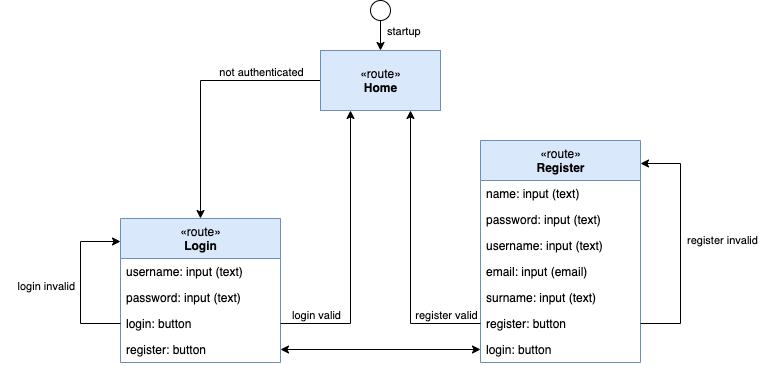
\includegraphics{ux-diagram/ux-auth.png}
      \caption{UX diagram for the authentication process.}
      \label{fig:ux-auth}
\end{figure}

\subsection{Home}
In Figure \ref{fig:ux-main} we outline the main flow of our application, starting from \textit{Home} page.
These interactions assume that the user is correctly logged in.

The \textit{Bottom Navigation Bar} component is used to navigate among the screens marked with the same \textit{``N''} symbol.

\begin{figure}[H]
      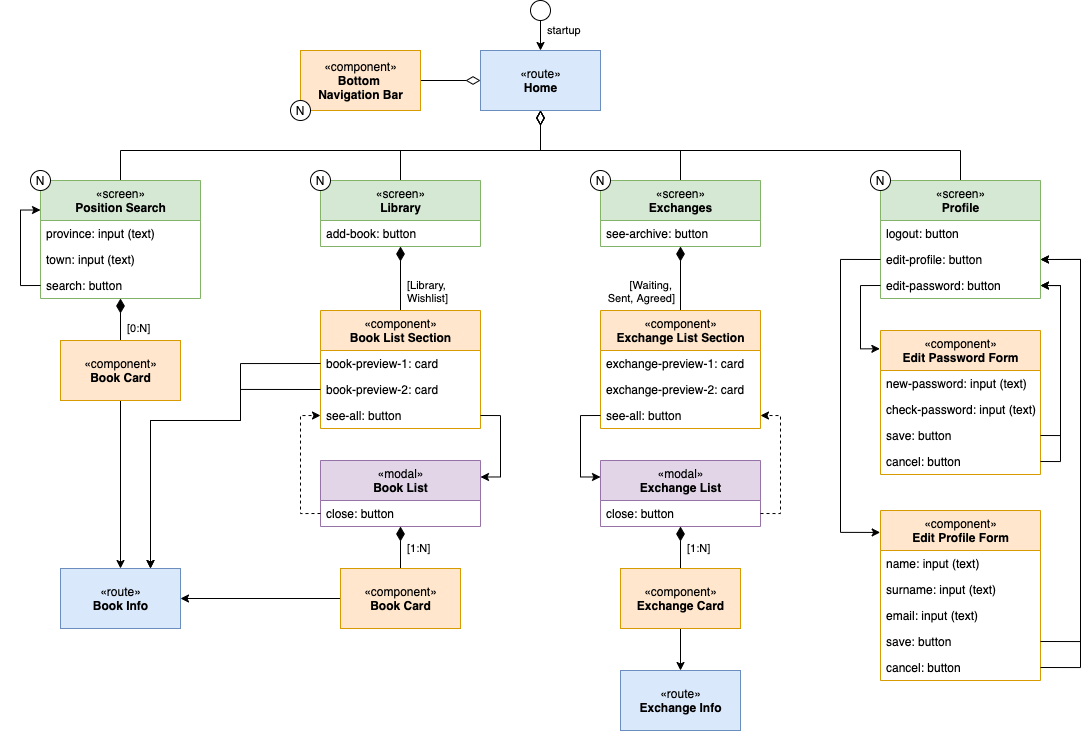
\includegraphics{ux-diagram/ux-part-1.png}
      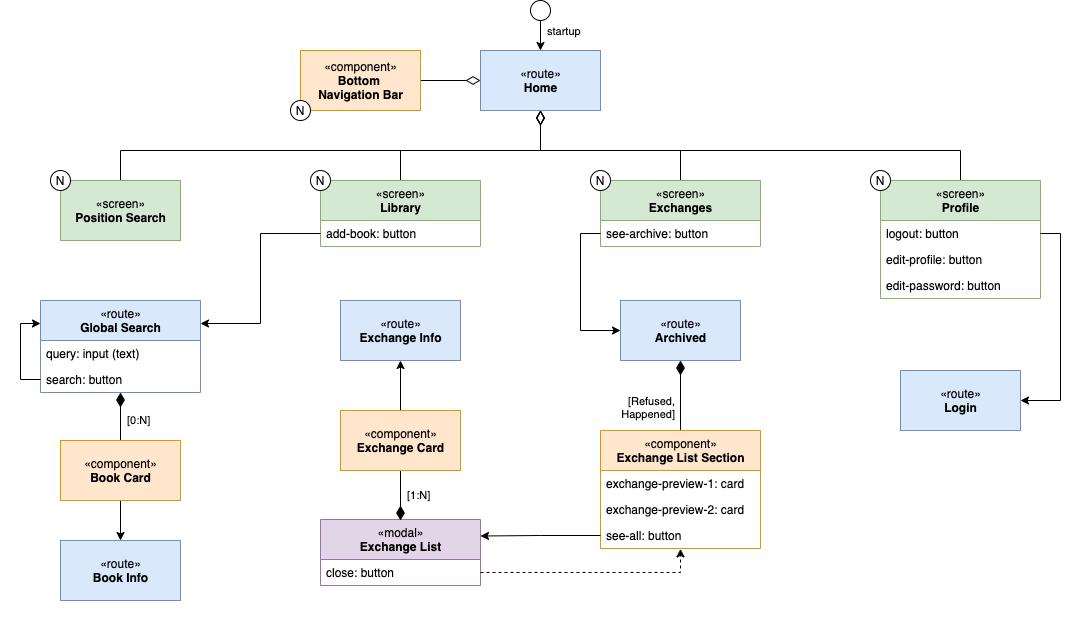
\includegraphics{ux-diagram/ux-part-2.png}
      \caption{UX diagram for the application.}
      \label{fig:ux-main}
\end{figure}

\subsection{Book and Exchange Info}
In Figure \ref{fig:ux-info} we expand \textit{Book Info} and \textit{Exchange Info} pages with all the actions that can be performed.
Note that only a subset of 1 to 3 actions will be available at each time.
These actions are selected dynamically depending on the state of the \texttt{Book} or \texttt{Exchange} object.

\begin{figure}[H]
      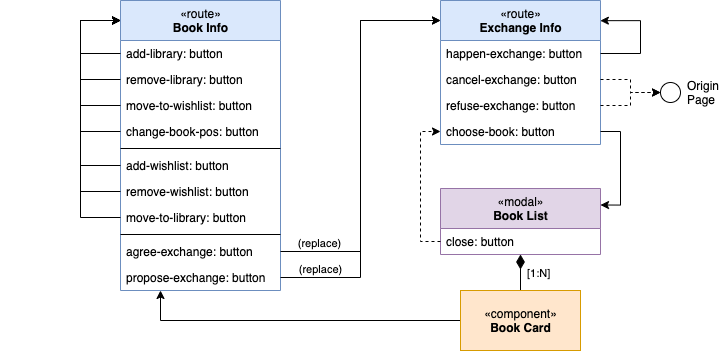
\includegraphics{ux-diagram/ux-info.png}
      \caption{UX diagram for the info pages.}
      \label{fig:ux-info}
\end{figure}

\clearpage
\section{Screenshots}
In this section instead, we want to show some screenshot from the actual implementation of our application.

\subsection{Login and Registration}
Both login and registration pages are structurally the same, they only differ on the number and type of fields.
The password field has the classical button (represented by the \textit{eye} icon) to show and hide its value.

\begin{figure}[H]
      \centering
      \makebox[\textwidth][c]{
            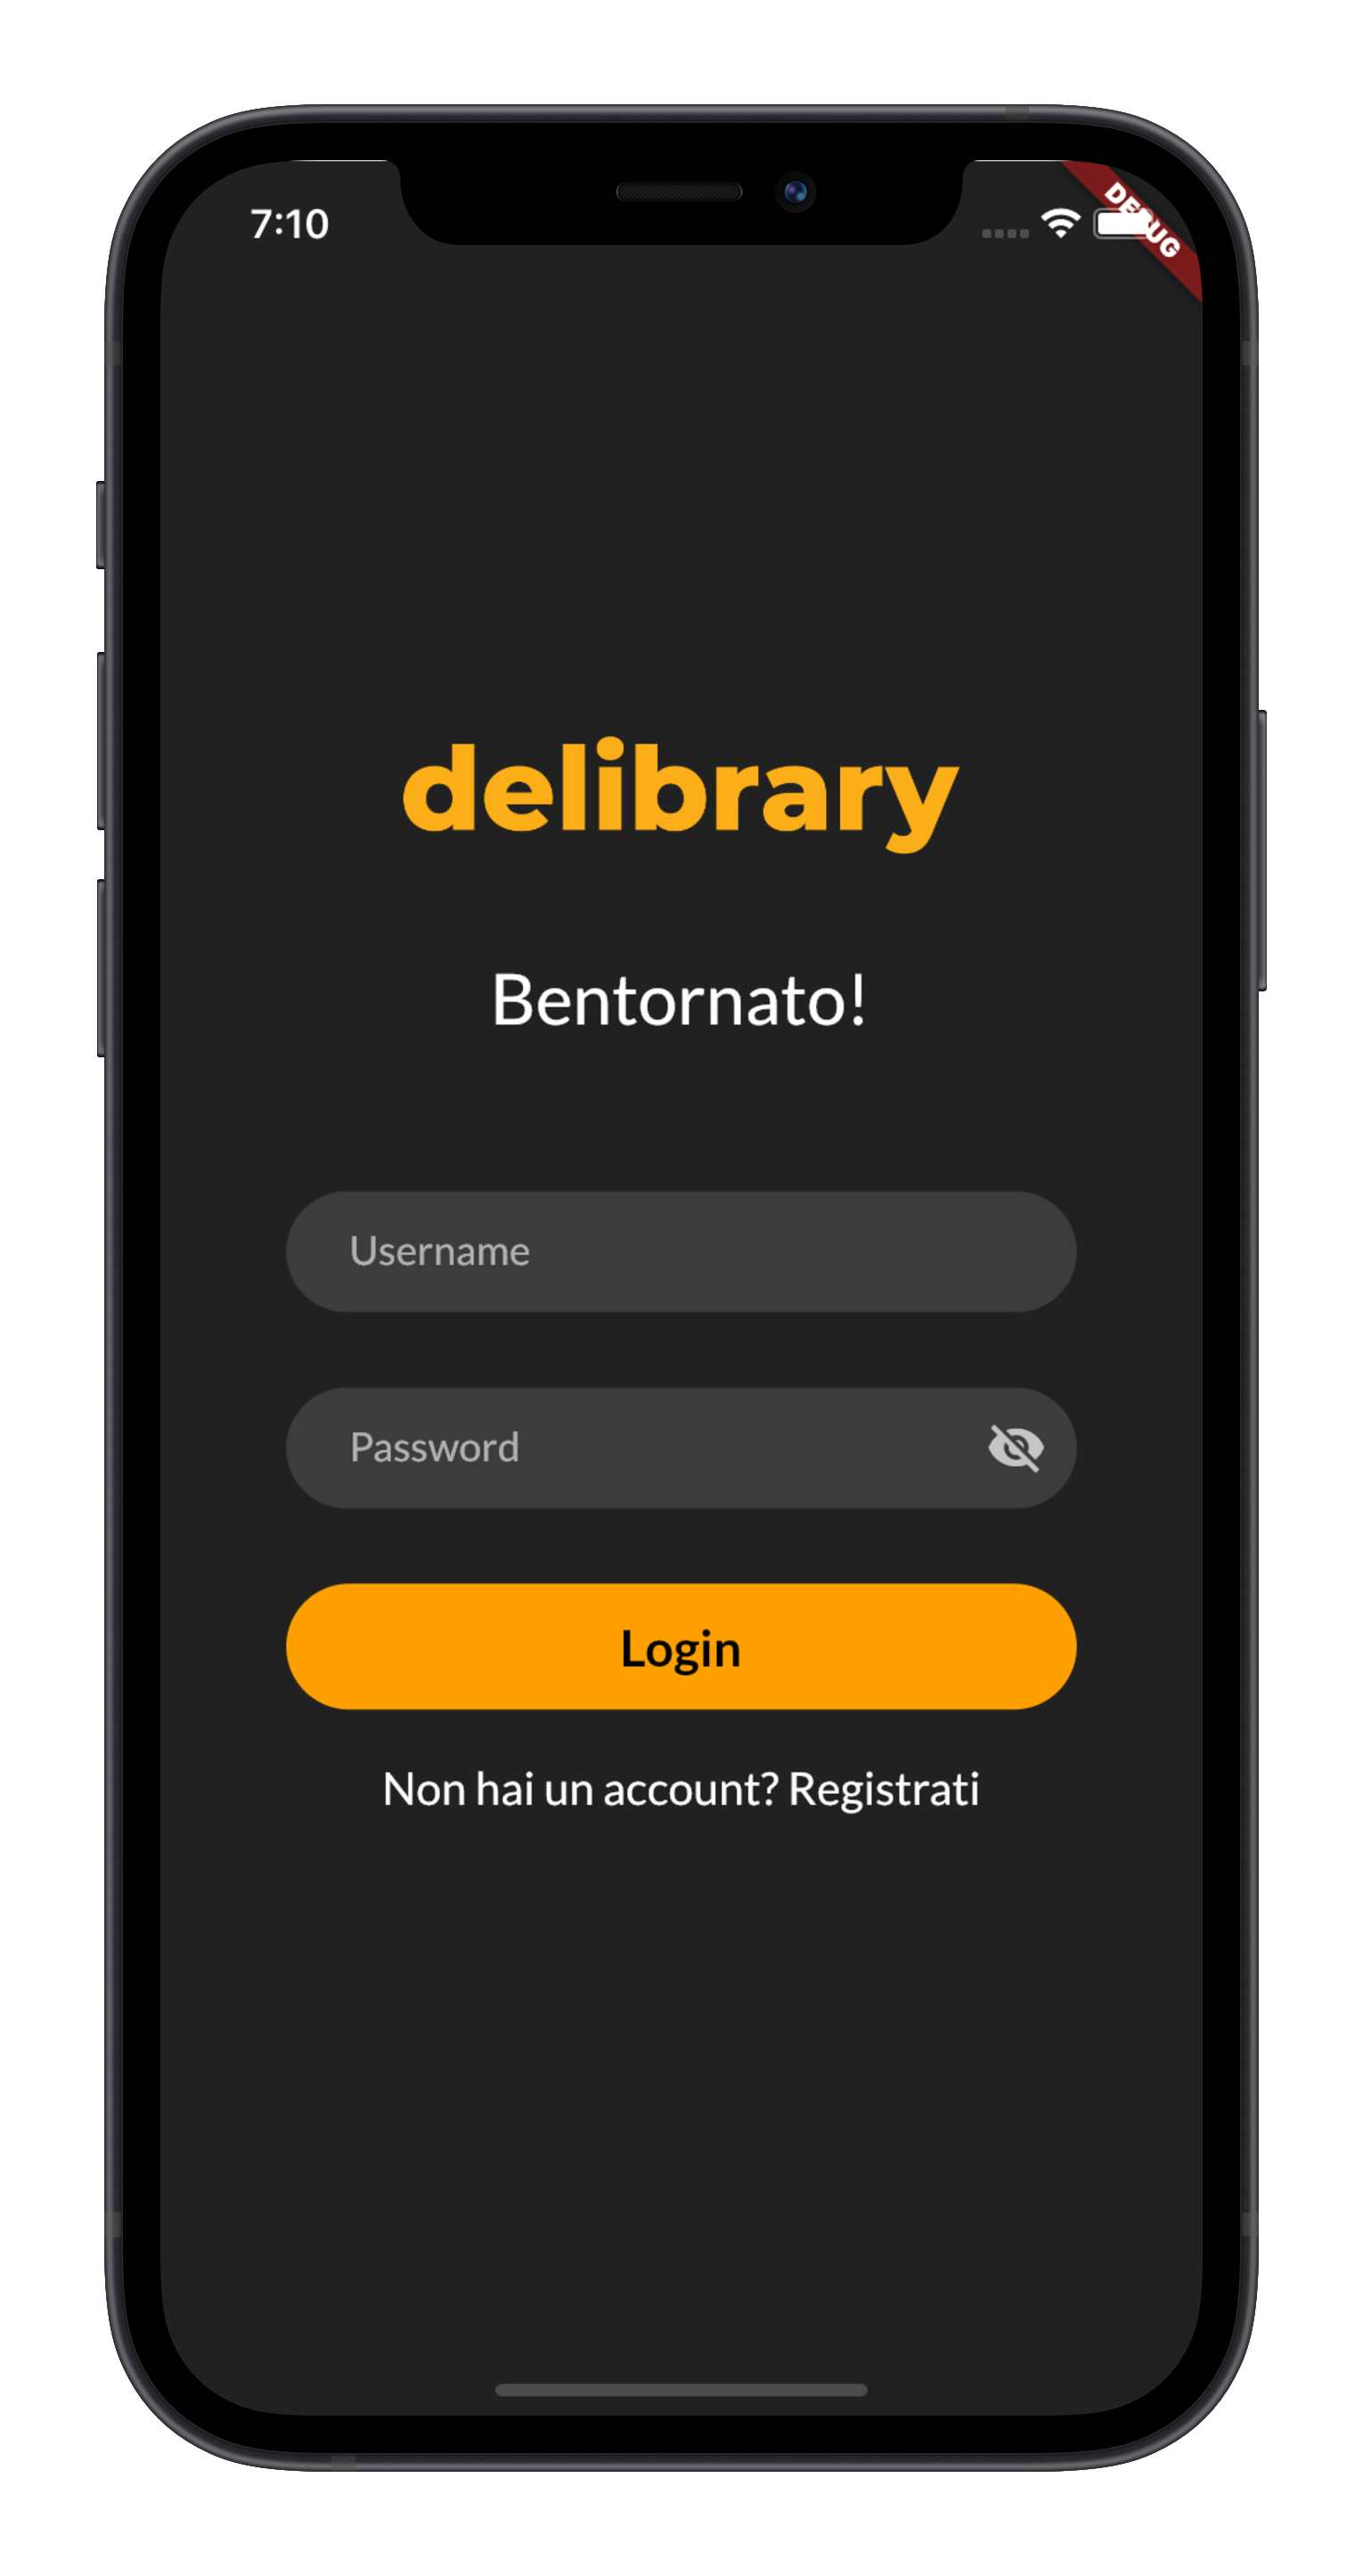
\includegraphics[width=0.35\textwidth]{screens/mock/smartphone/login.png}
            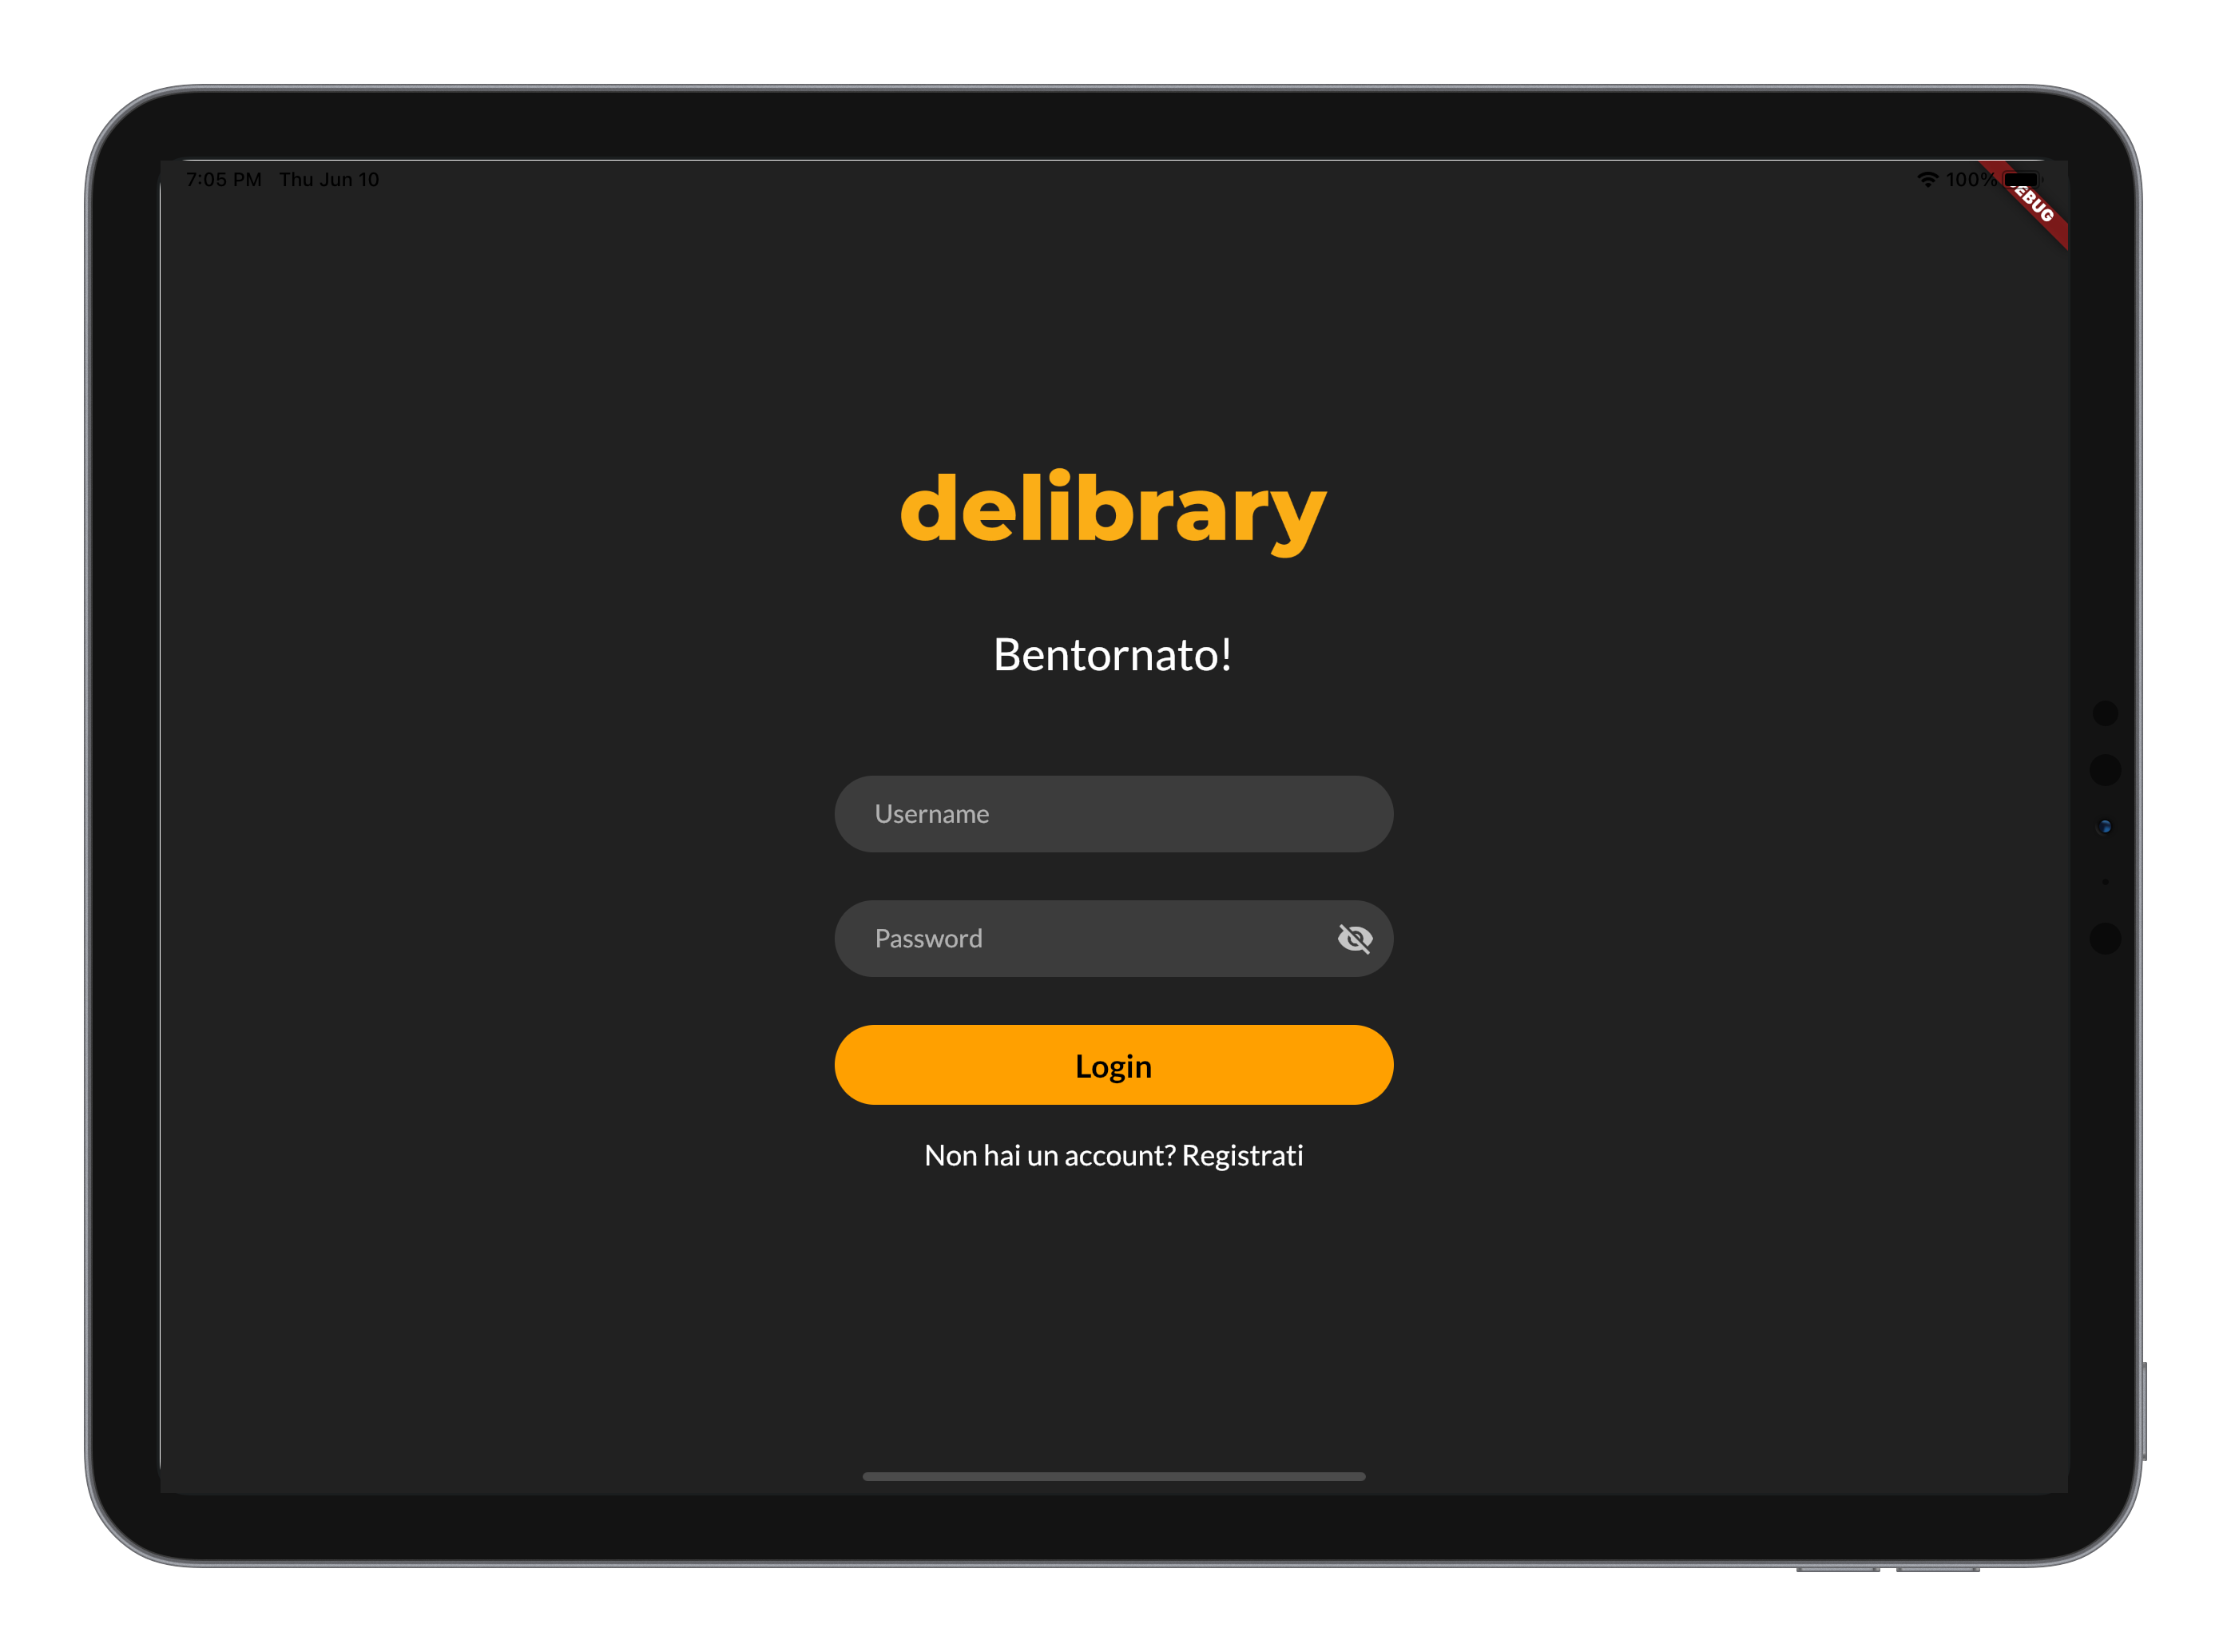
\includegraphics[width=0.75\textwidth]{screens/mock/tablet-landscape/login.png}
      }
      \caption{Login page}
\end{figure}

\clearpage
\subsection{Global and Position Search}
Results of the user's query are shown in a \texttt{CustomScrollView} designed to fit the size of the device.
As it is possible to see, in fact, the cards are arranged in a grid whose columns change with the width of the screen.
Moreover, we implemented the search block as a \texttt{SliverAppBar} that slides out of the screen 
as soon as the user starts scrolling and can then be reached by moving upwards.

\begin{figure}[H]
      \centering
      \makebox[\textwidth][c]{
            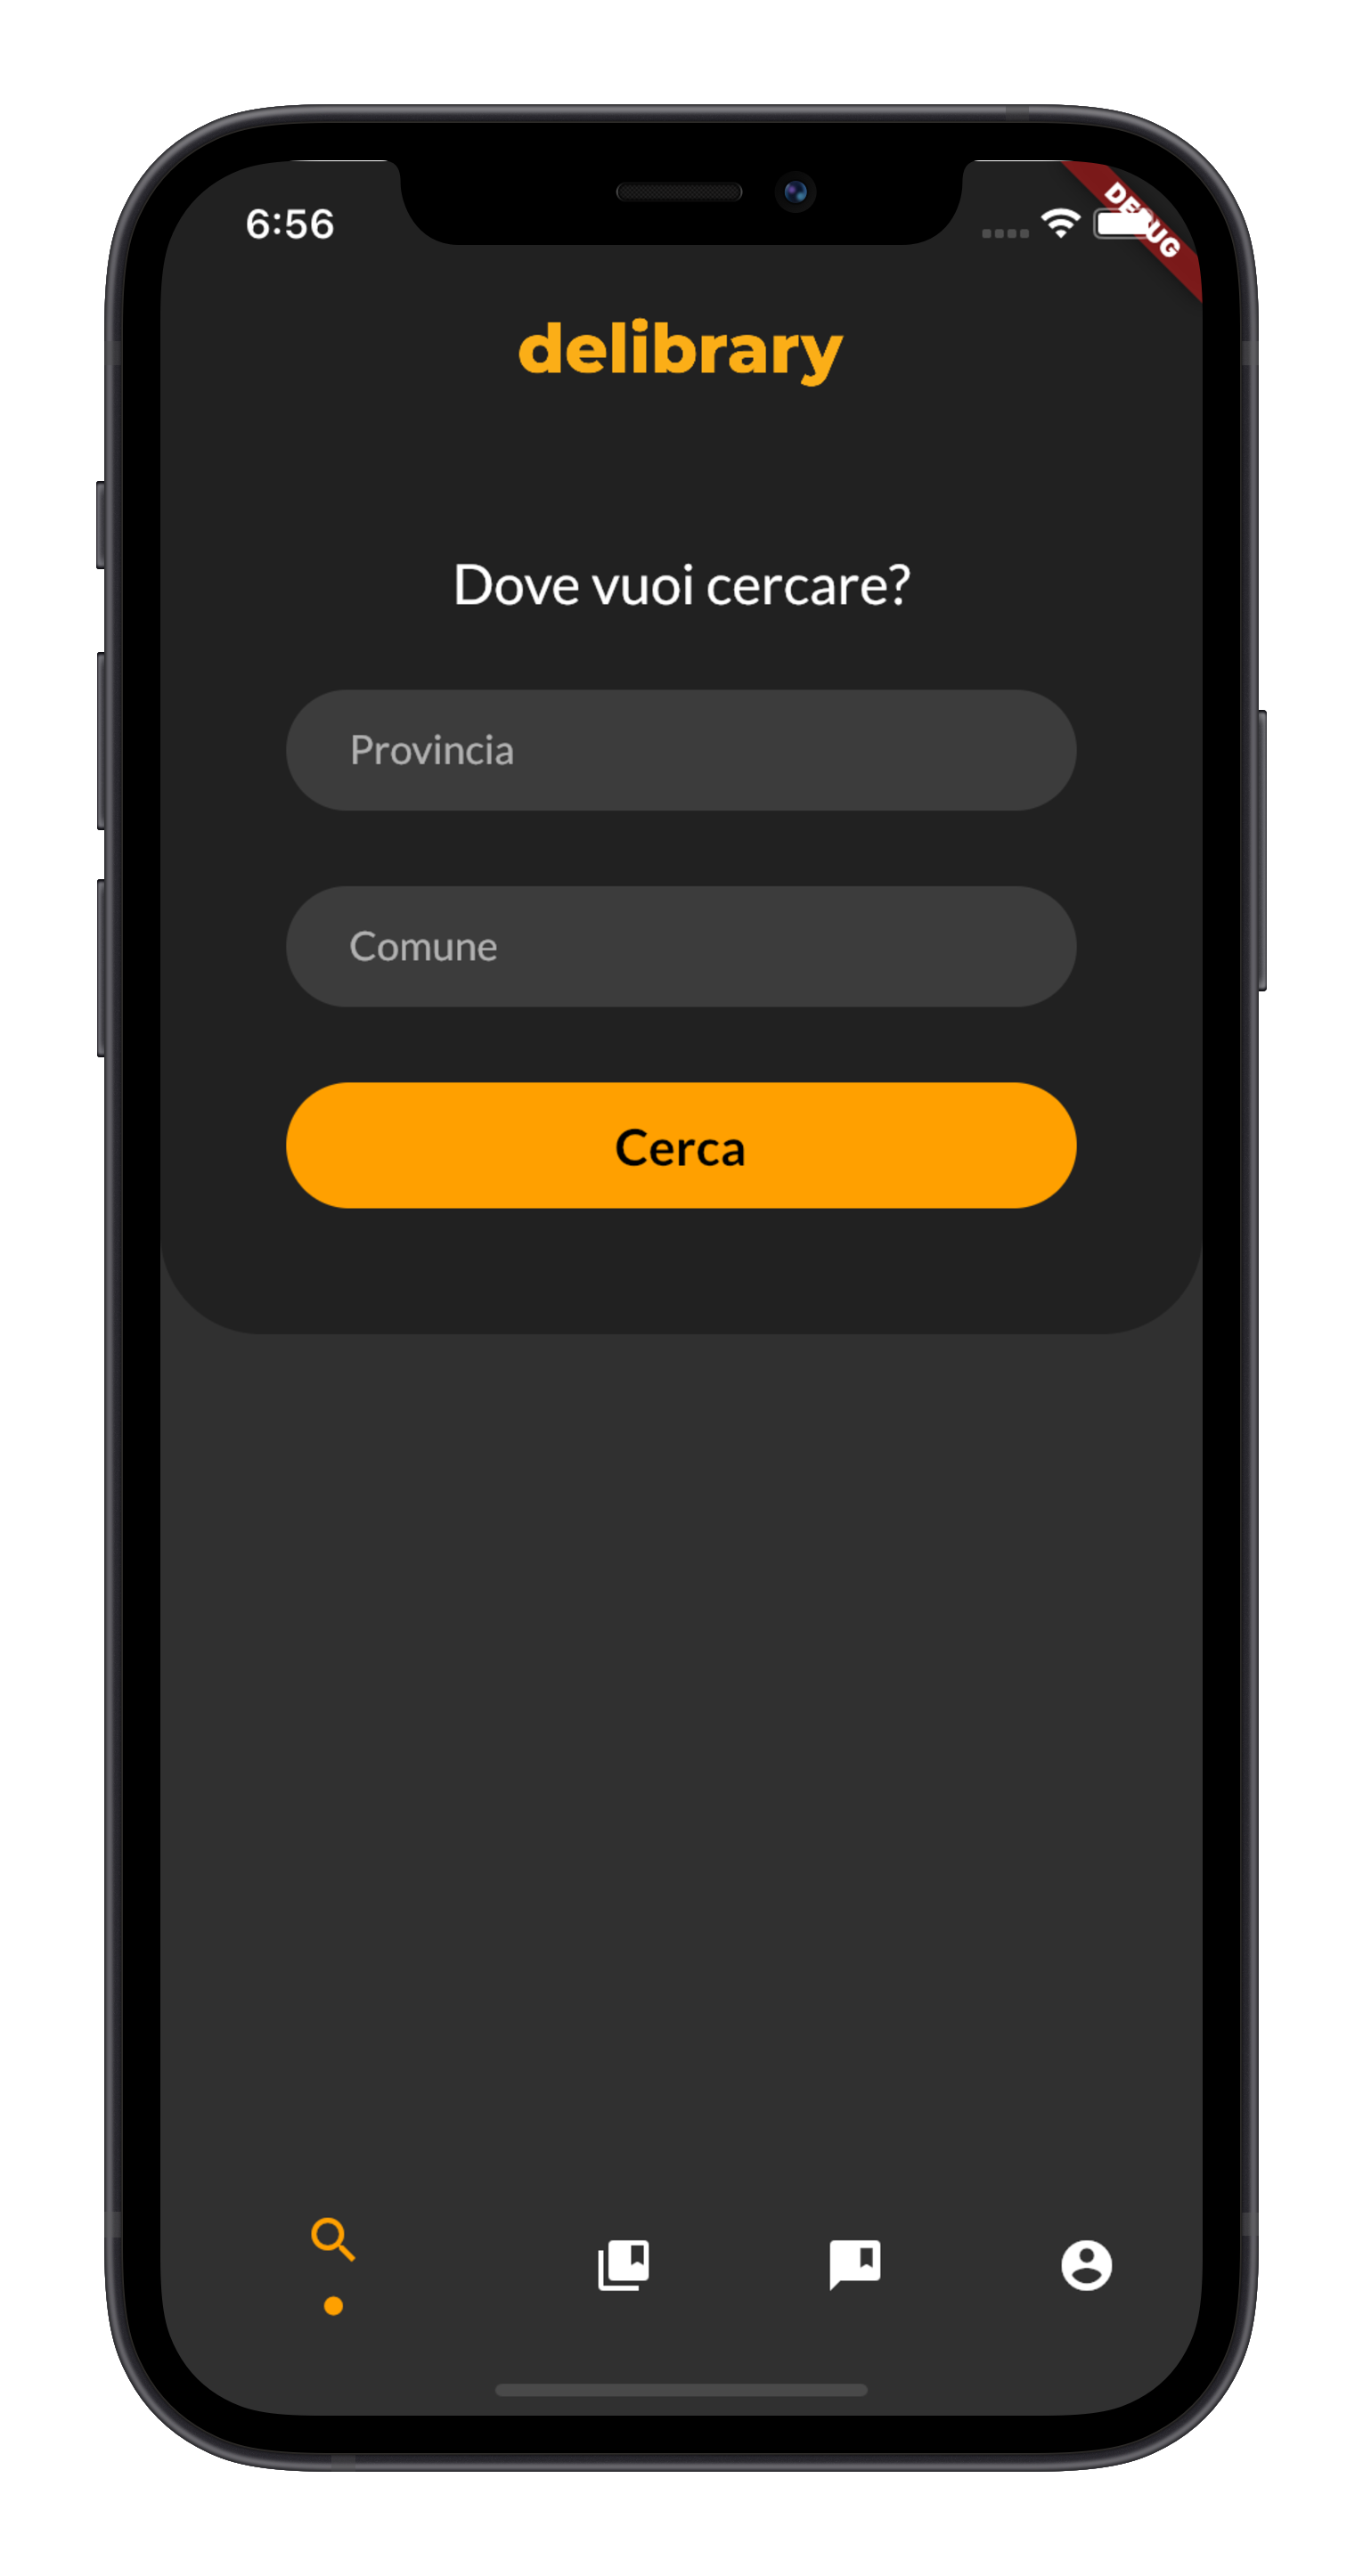
\includegraphics[width=0.35\textwidth]{screens/mock/smartphone/position-search-empty.png}
            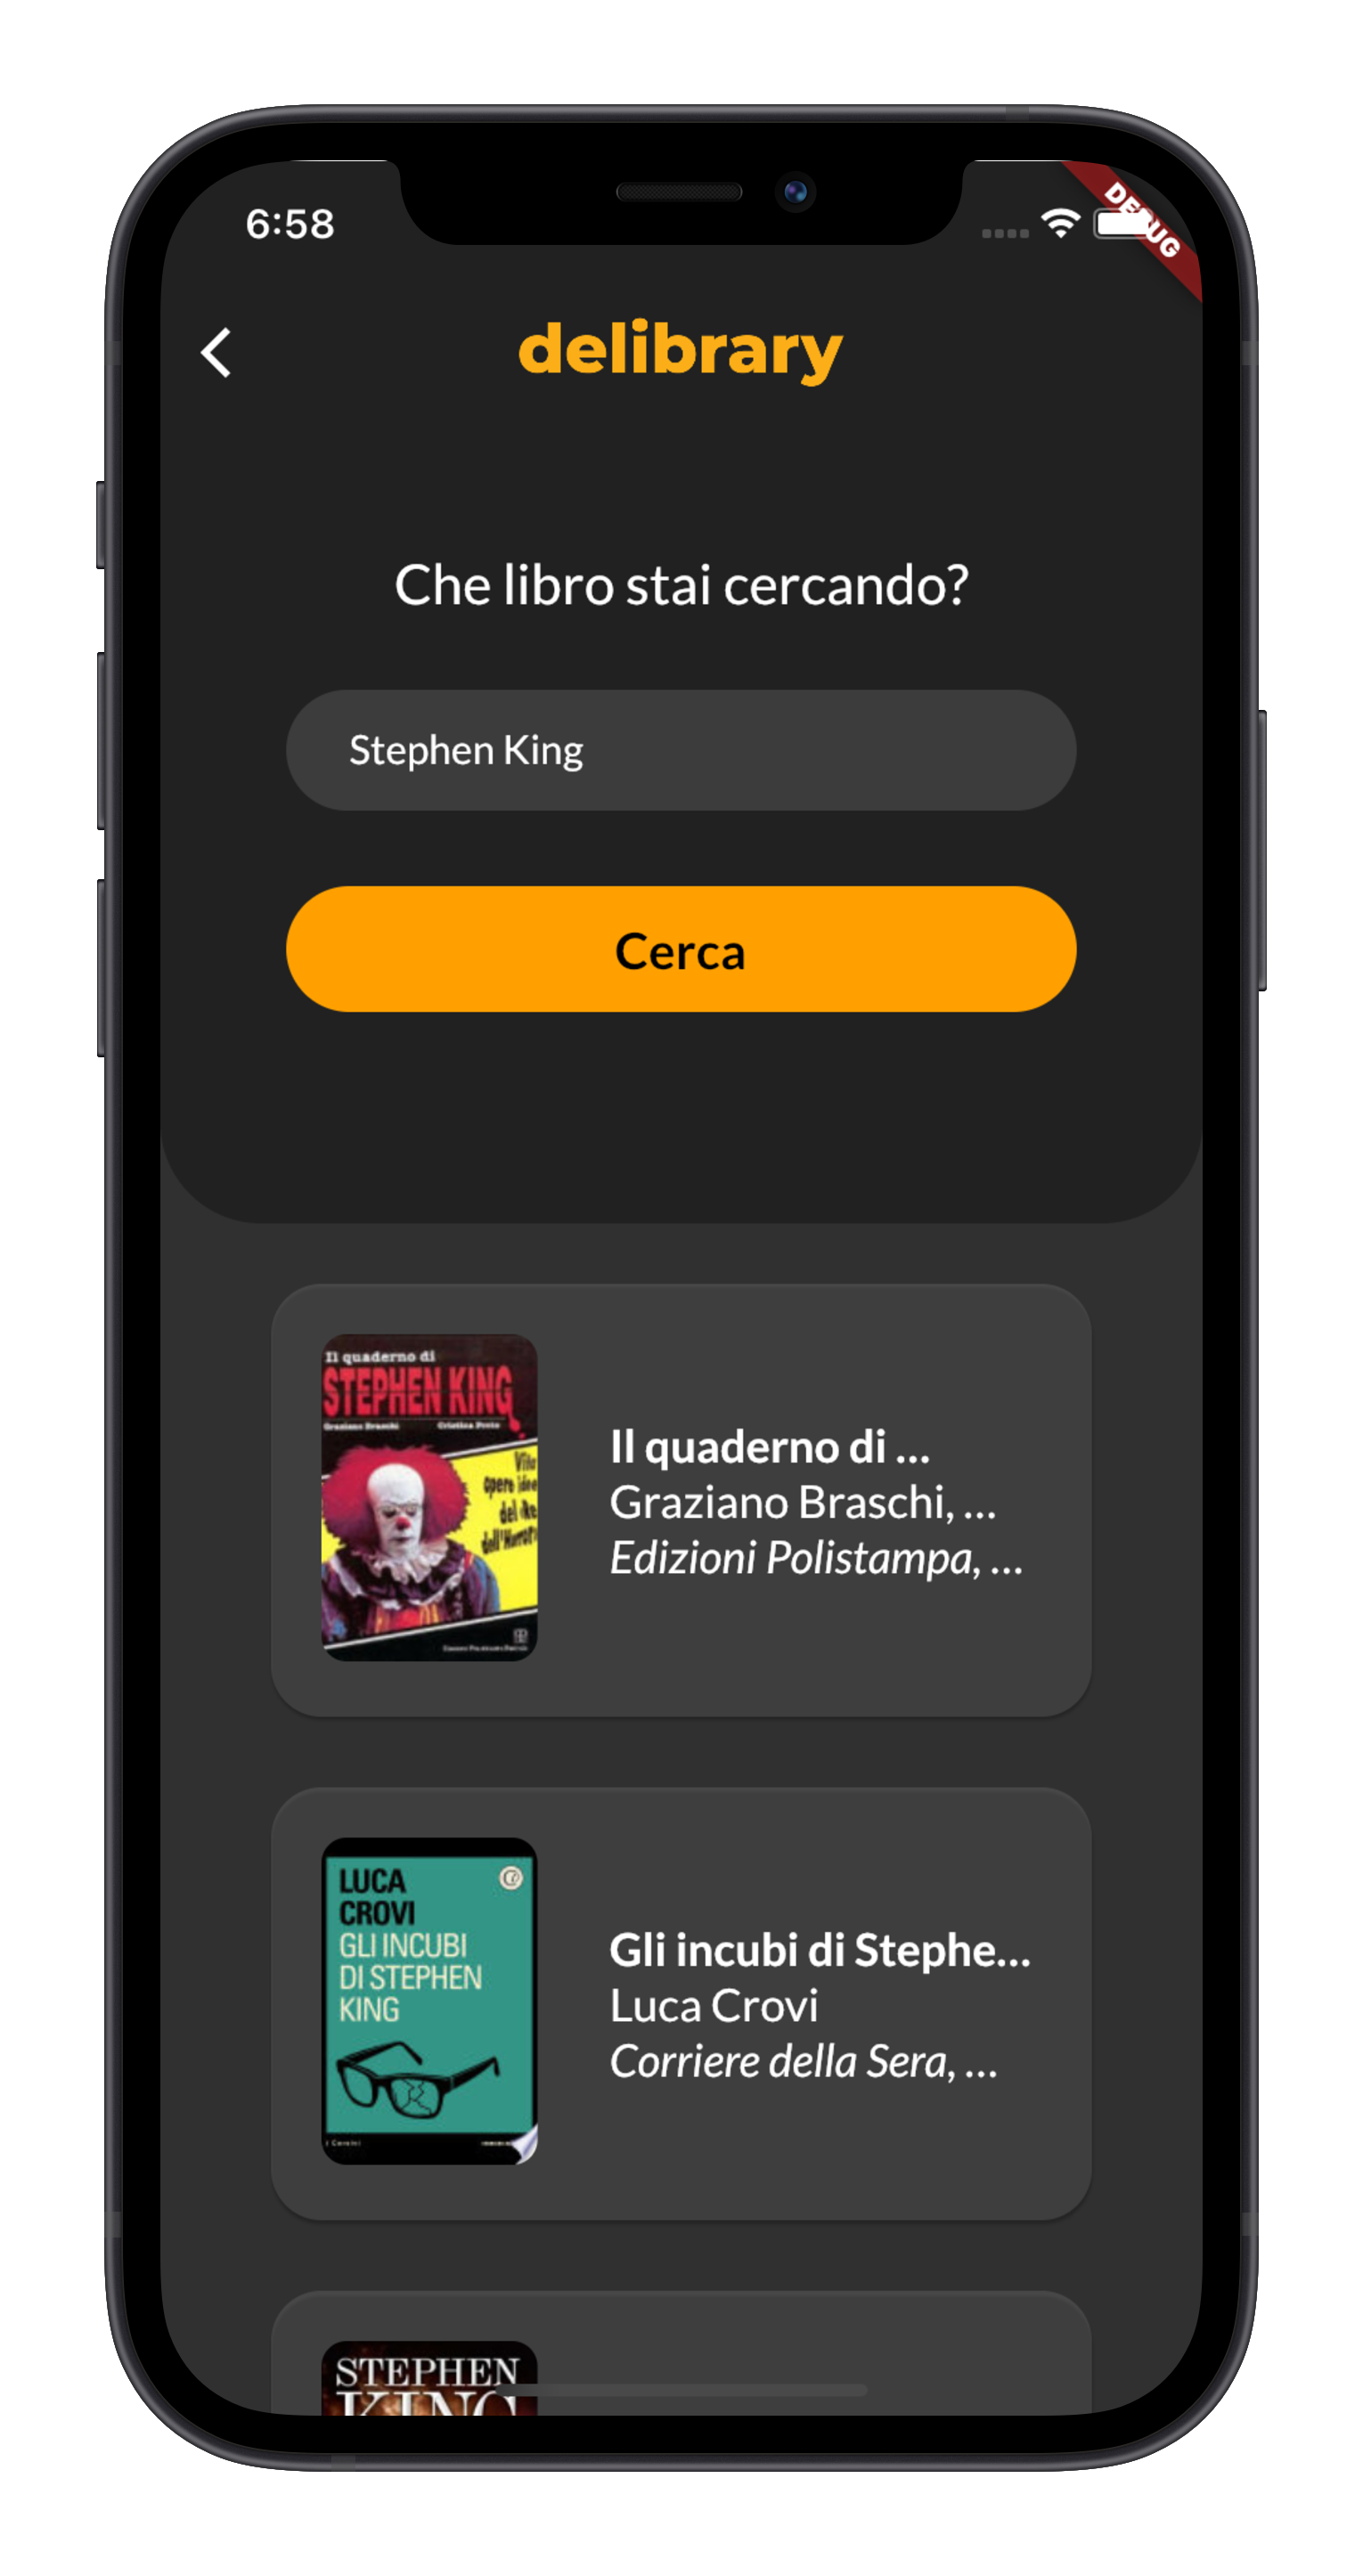
\includegraphics[width=0.35\textwidth]{screens/mock/smartphone/global-search-filled.png}
            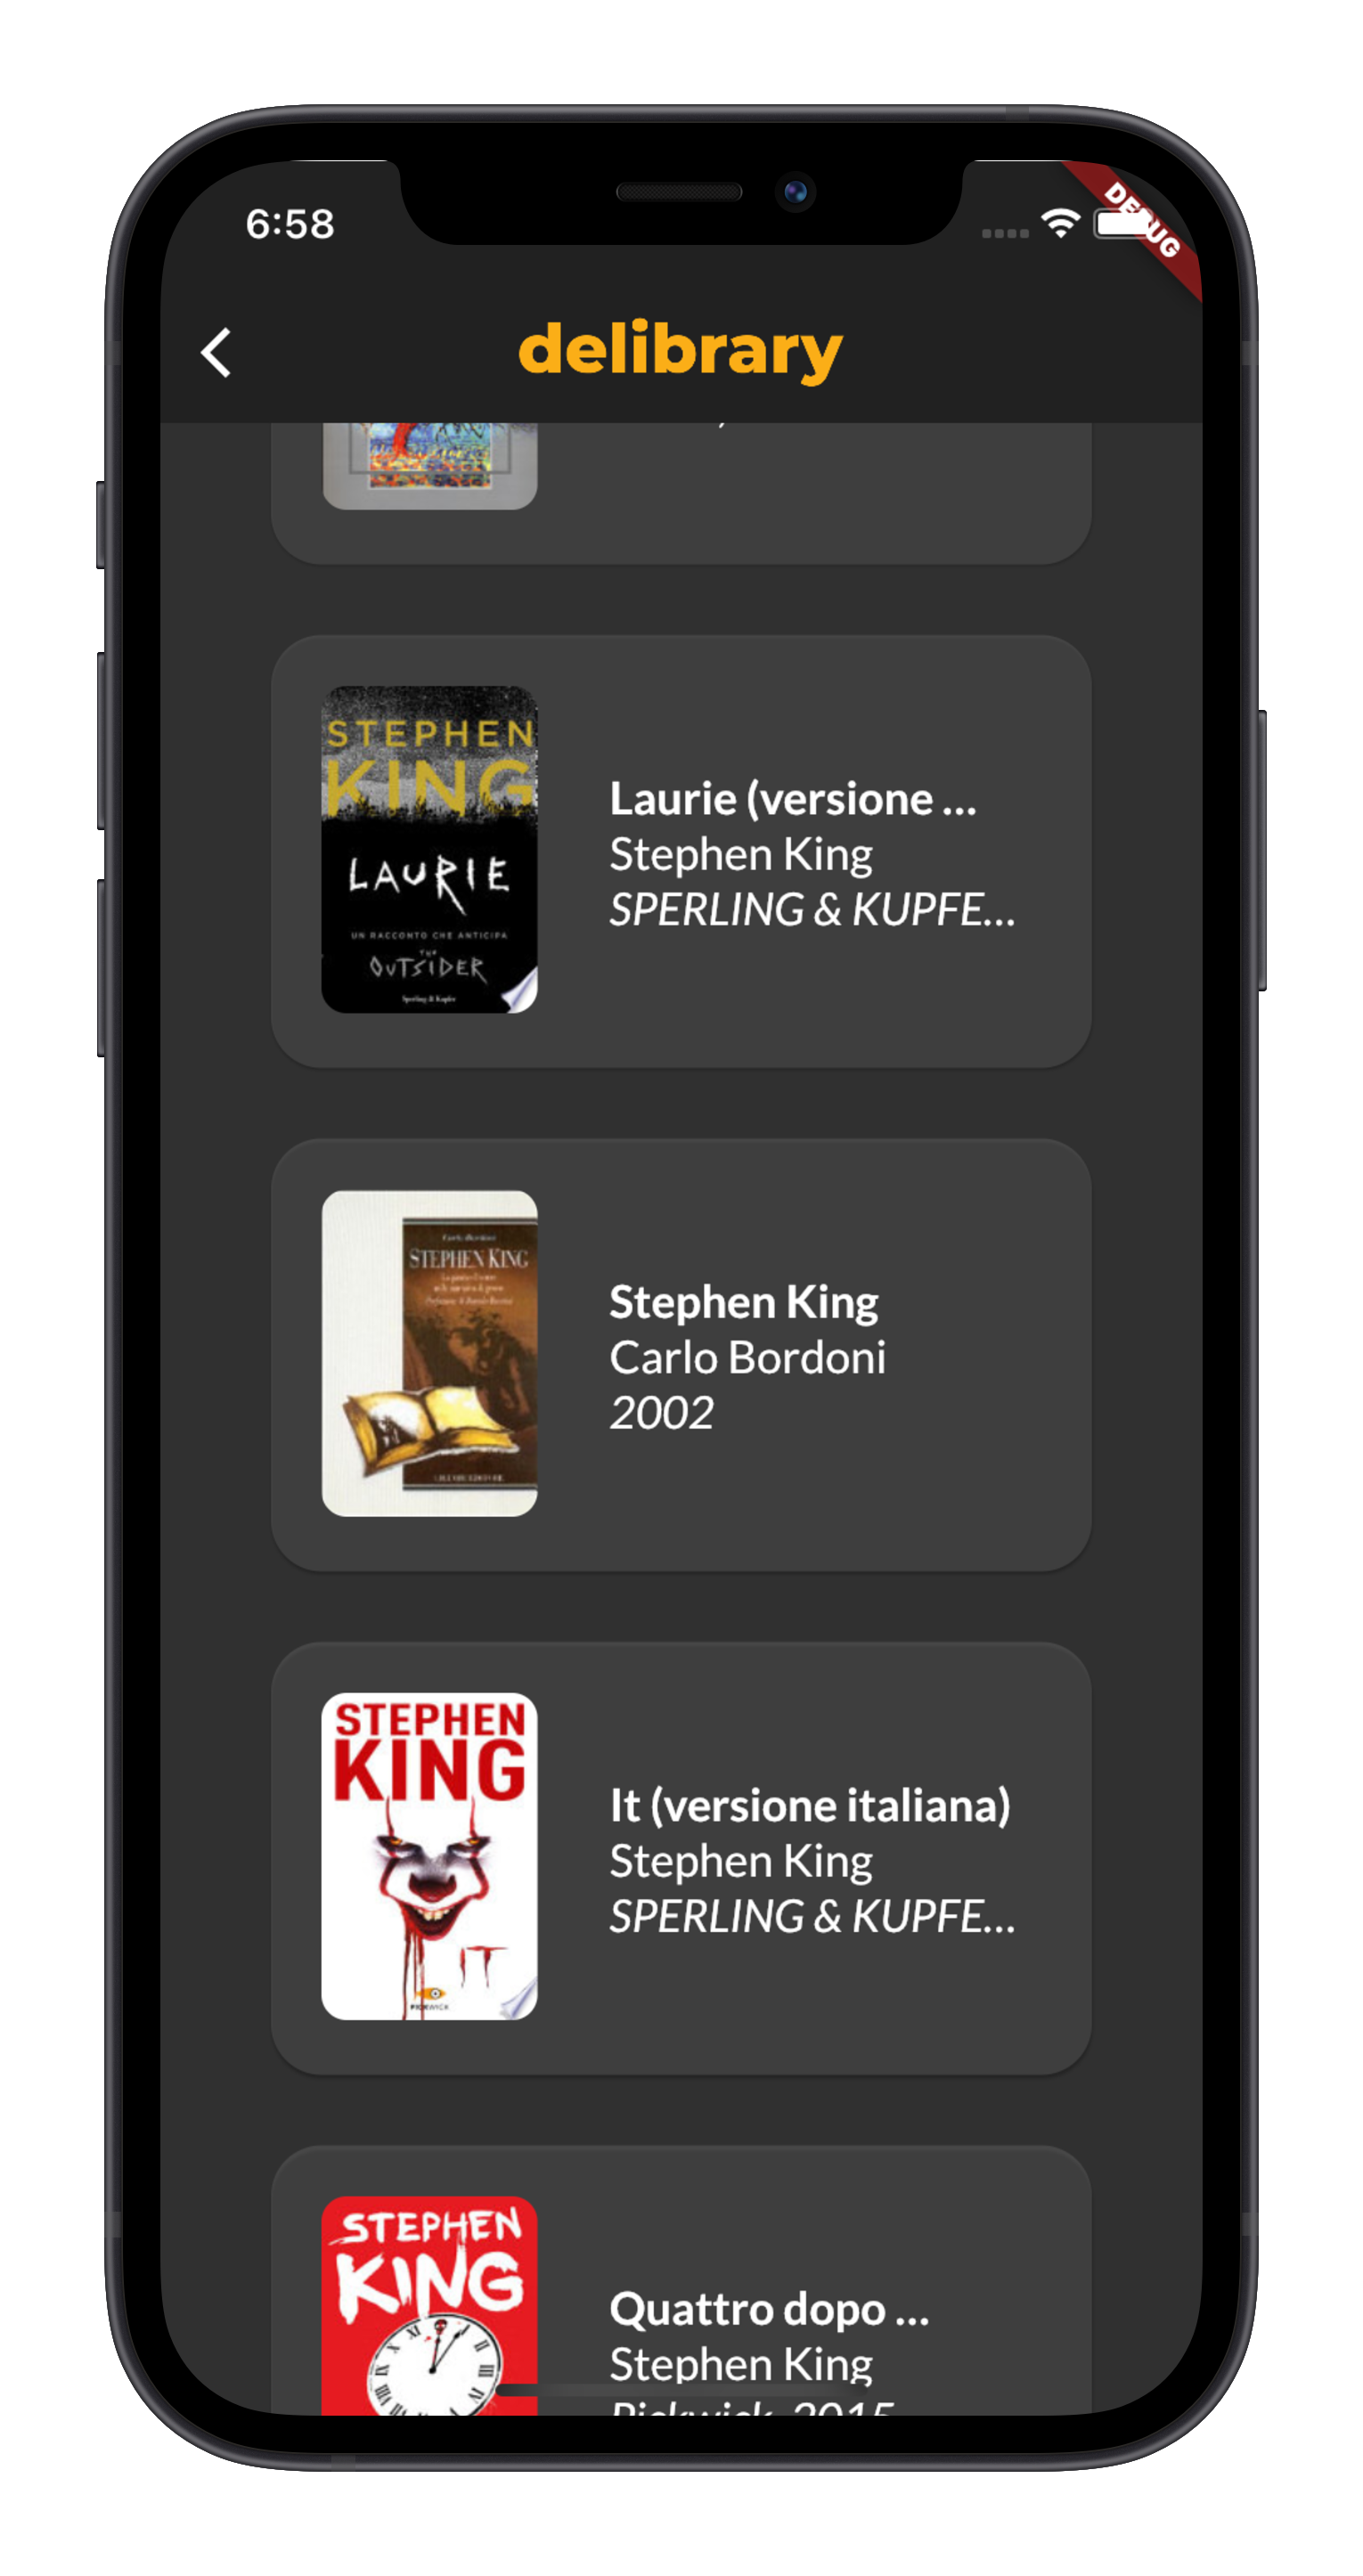
\includegraphics[width=0.35\textwidth]{screens/mock/smartphone/global-search-scrolled.png}
      }
      \makebox[\textwidth][c]{
            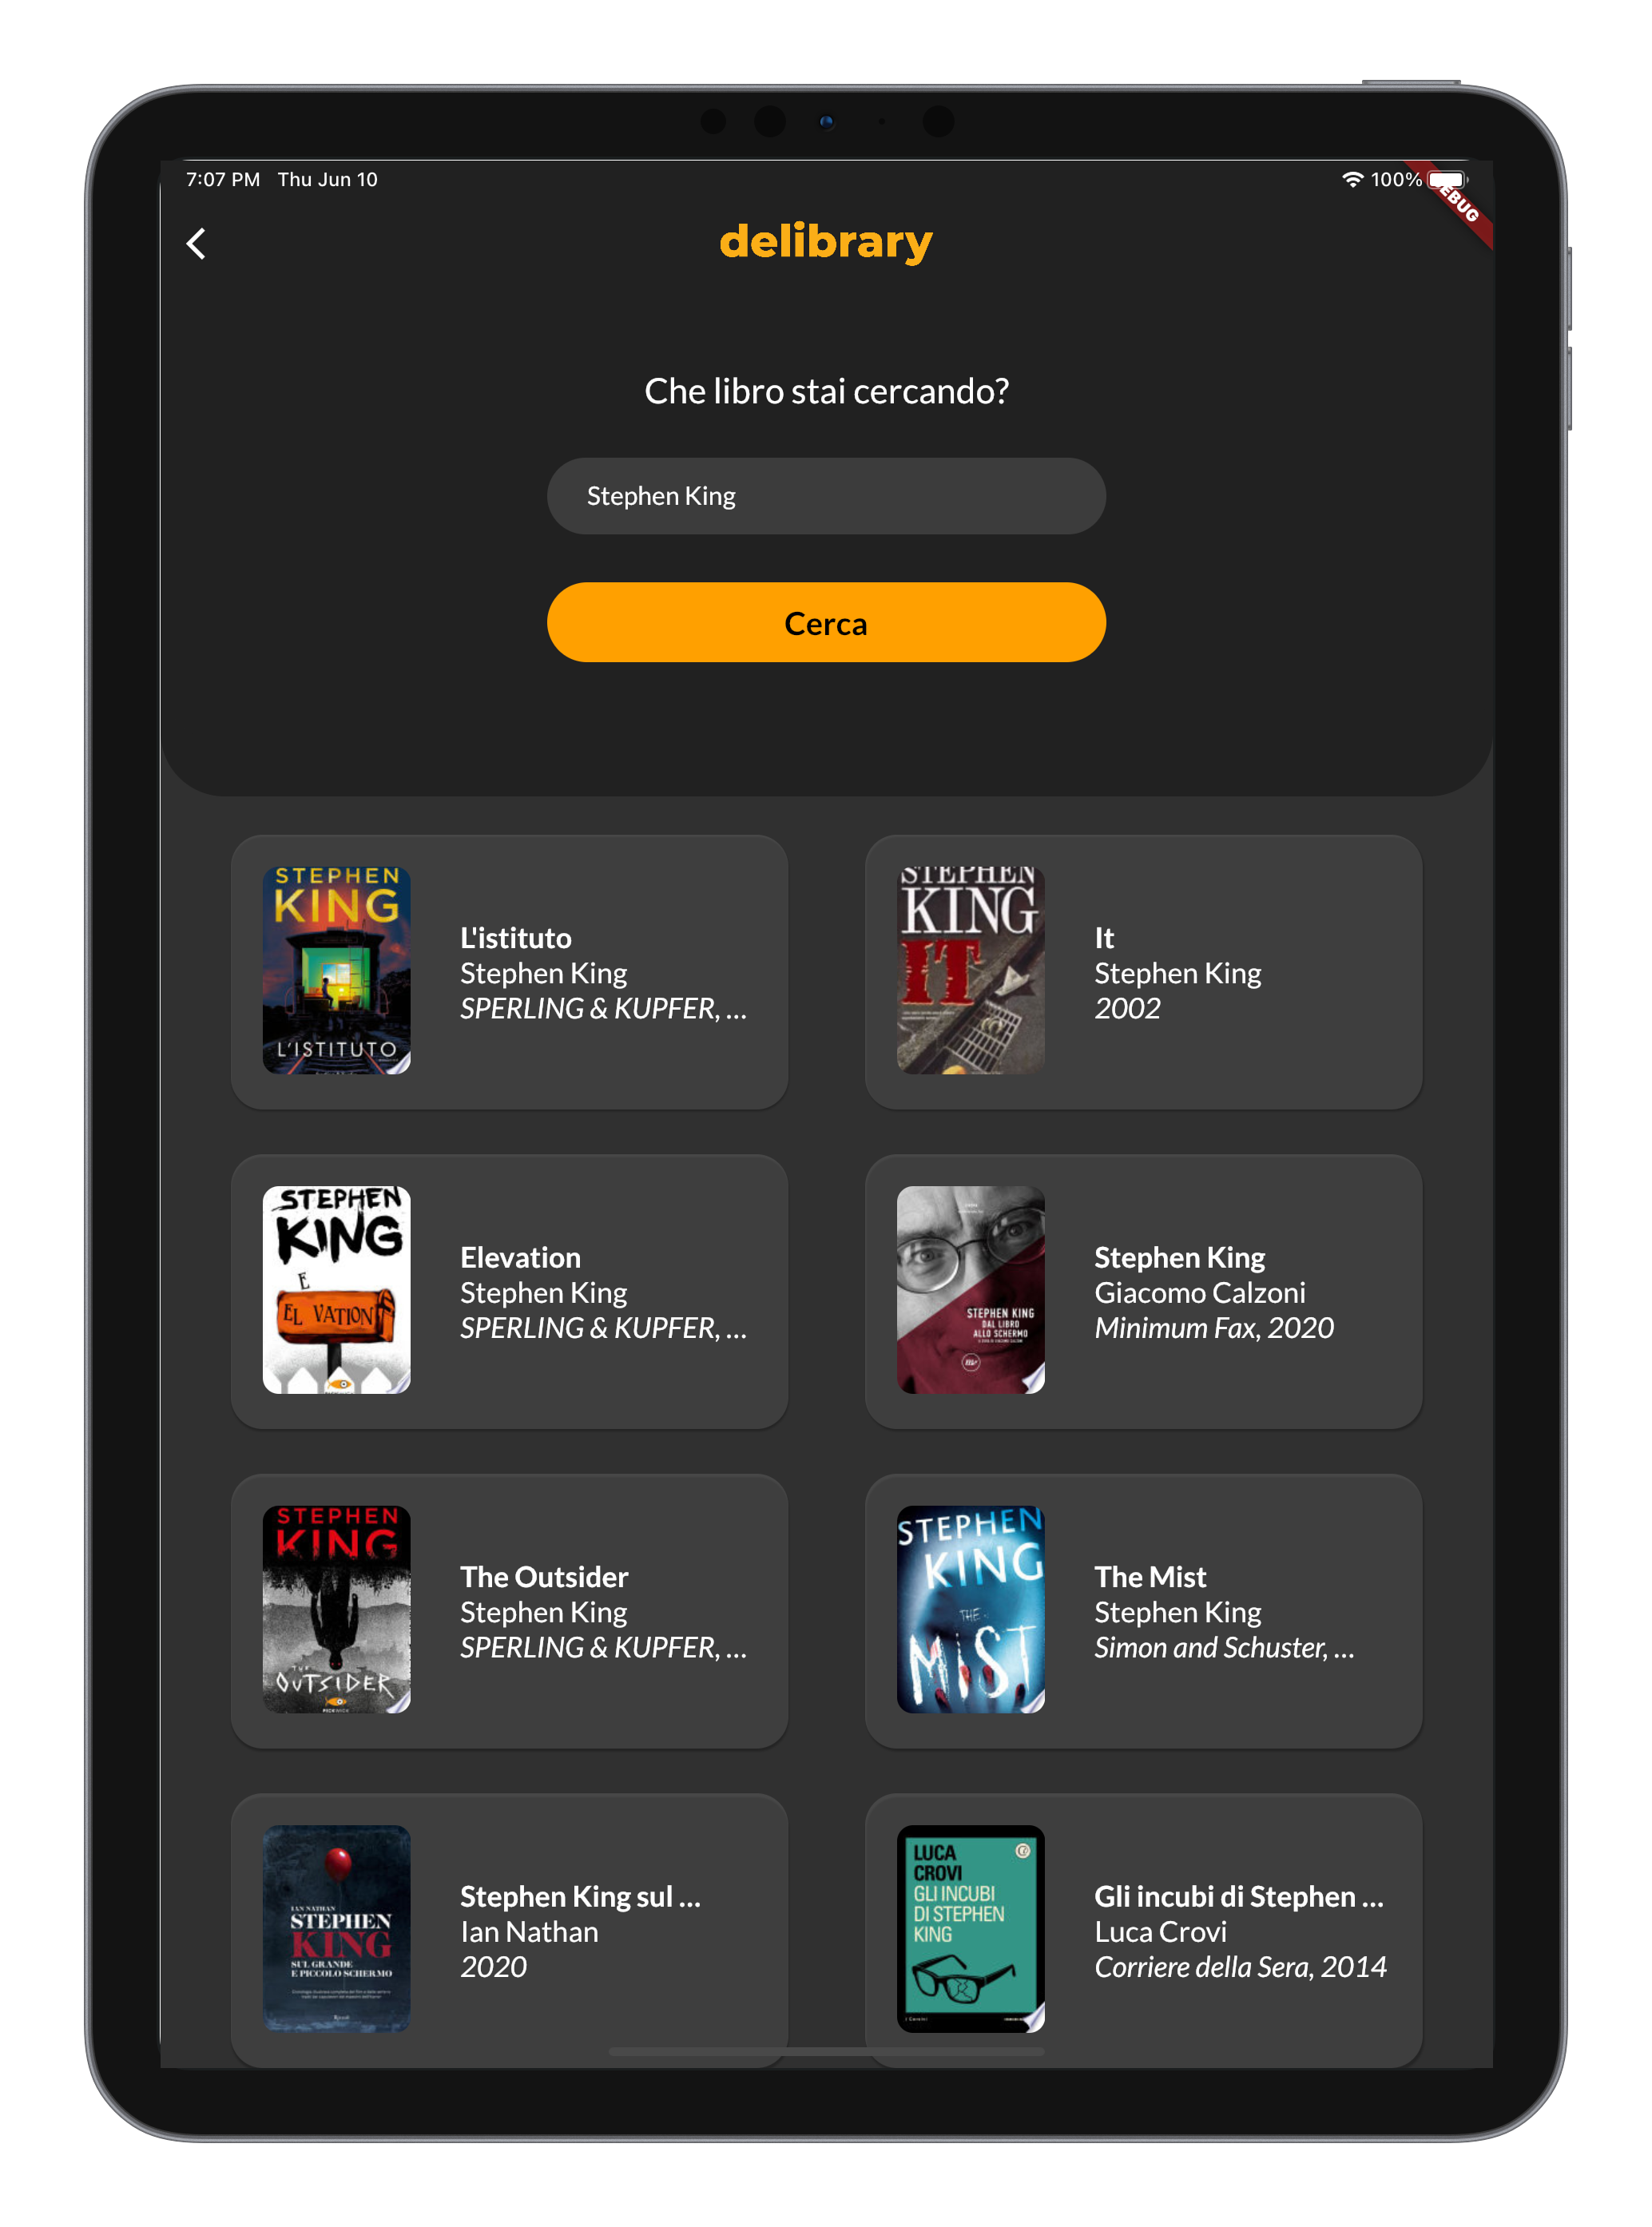
\includegraphics[width=0.44\textwidth]{screens/mock/tablet-portrait/global-search-filled.png}
            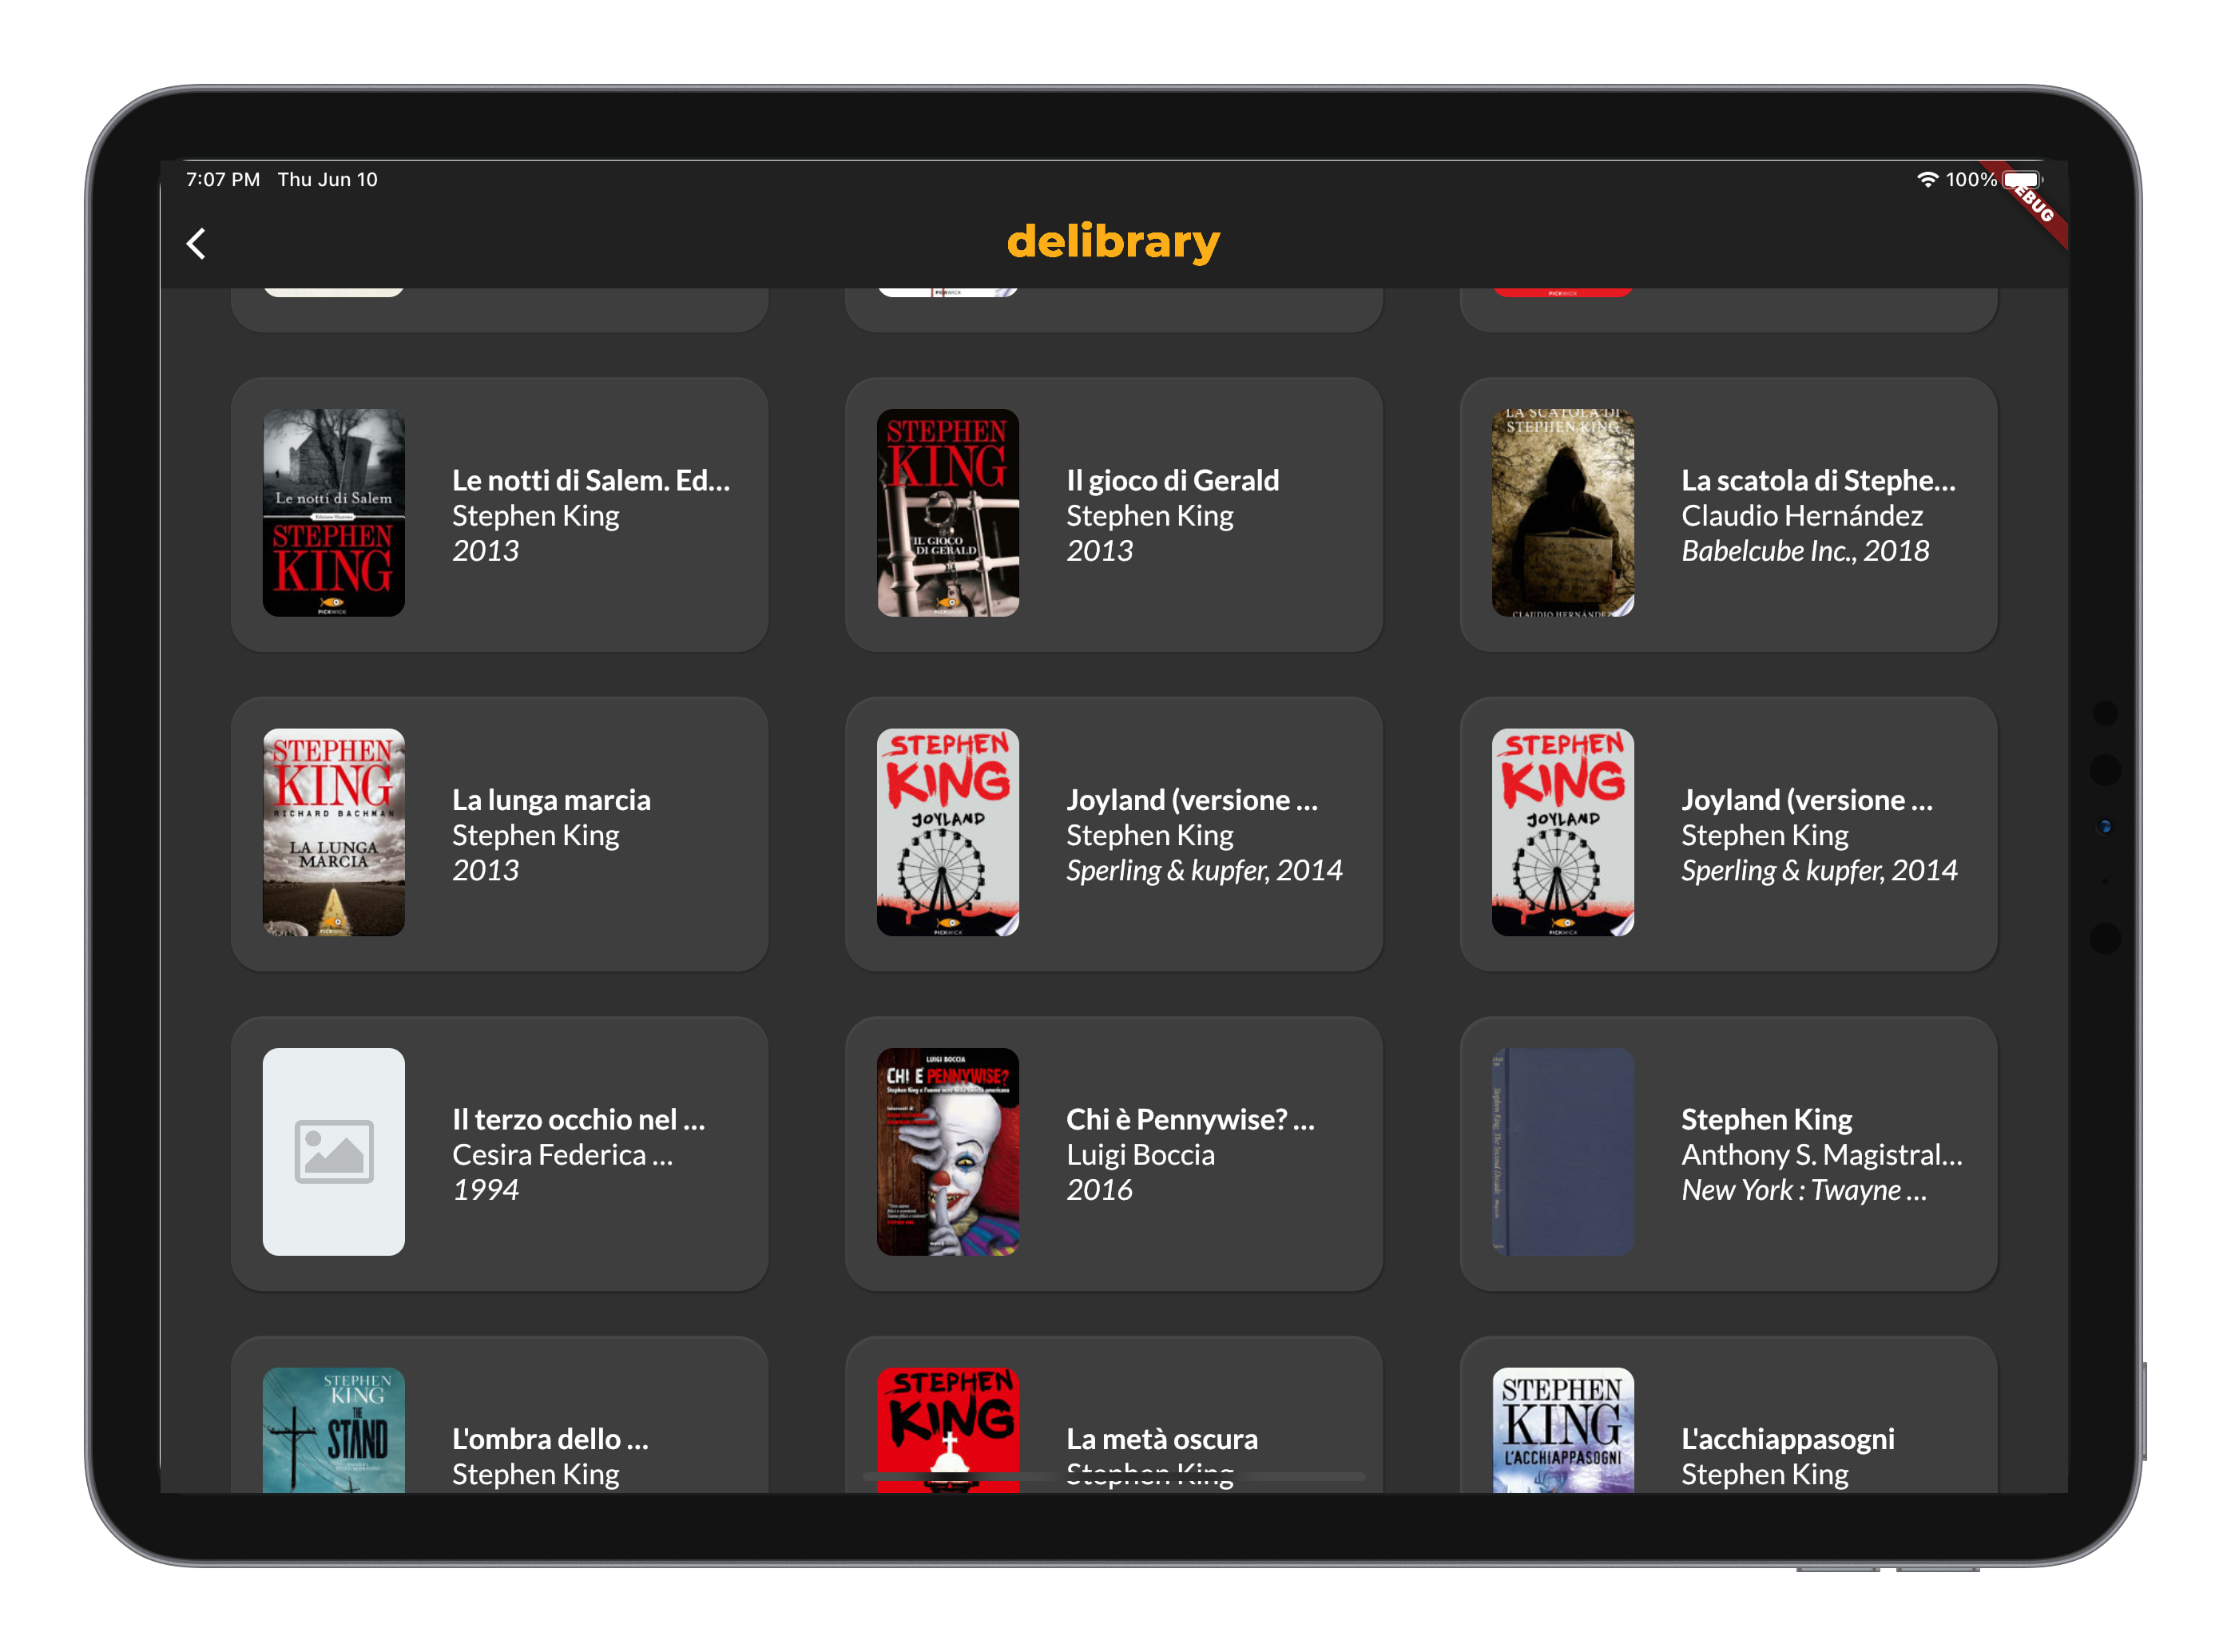
\includegraphics[width=0.65\textwidth]{screens/mock/tablet-landscape/global-search-scrolled.png}
      }
      \caption{Position and global search pages}
\end{figure}

\clearpage
\subsection{Library, Exchanges and Archive}
Again, these pages have the same structure. Books are grouped in library and wishlist, while exchanges are grouped depending on their state.\\
Each group displays up to two clickable previews and a button.
When the button is tapped, the application shows a modal with the whole list of cards.
Also in this case, the interface is able to adapt to the size of the device.

\begin{figure}[H]
      \centering
      \makebox[\textwidth][c]{
            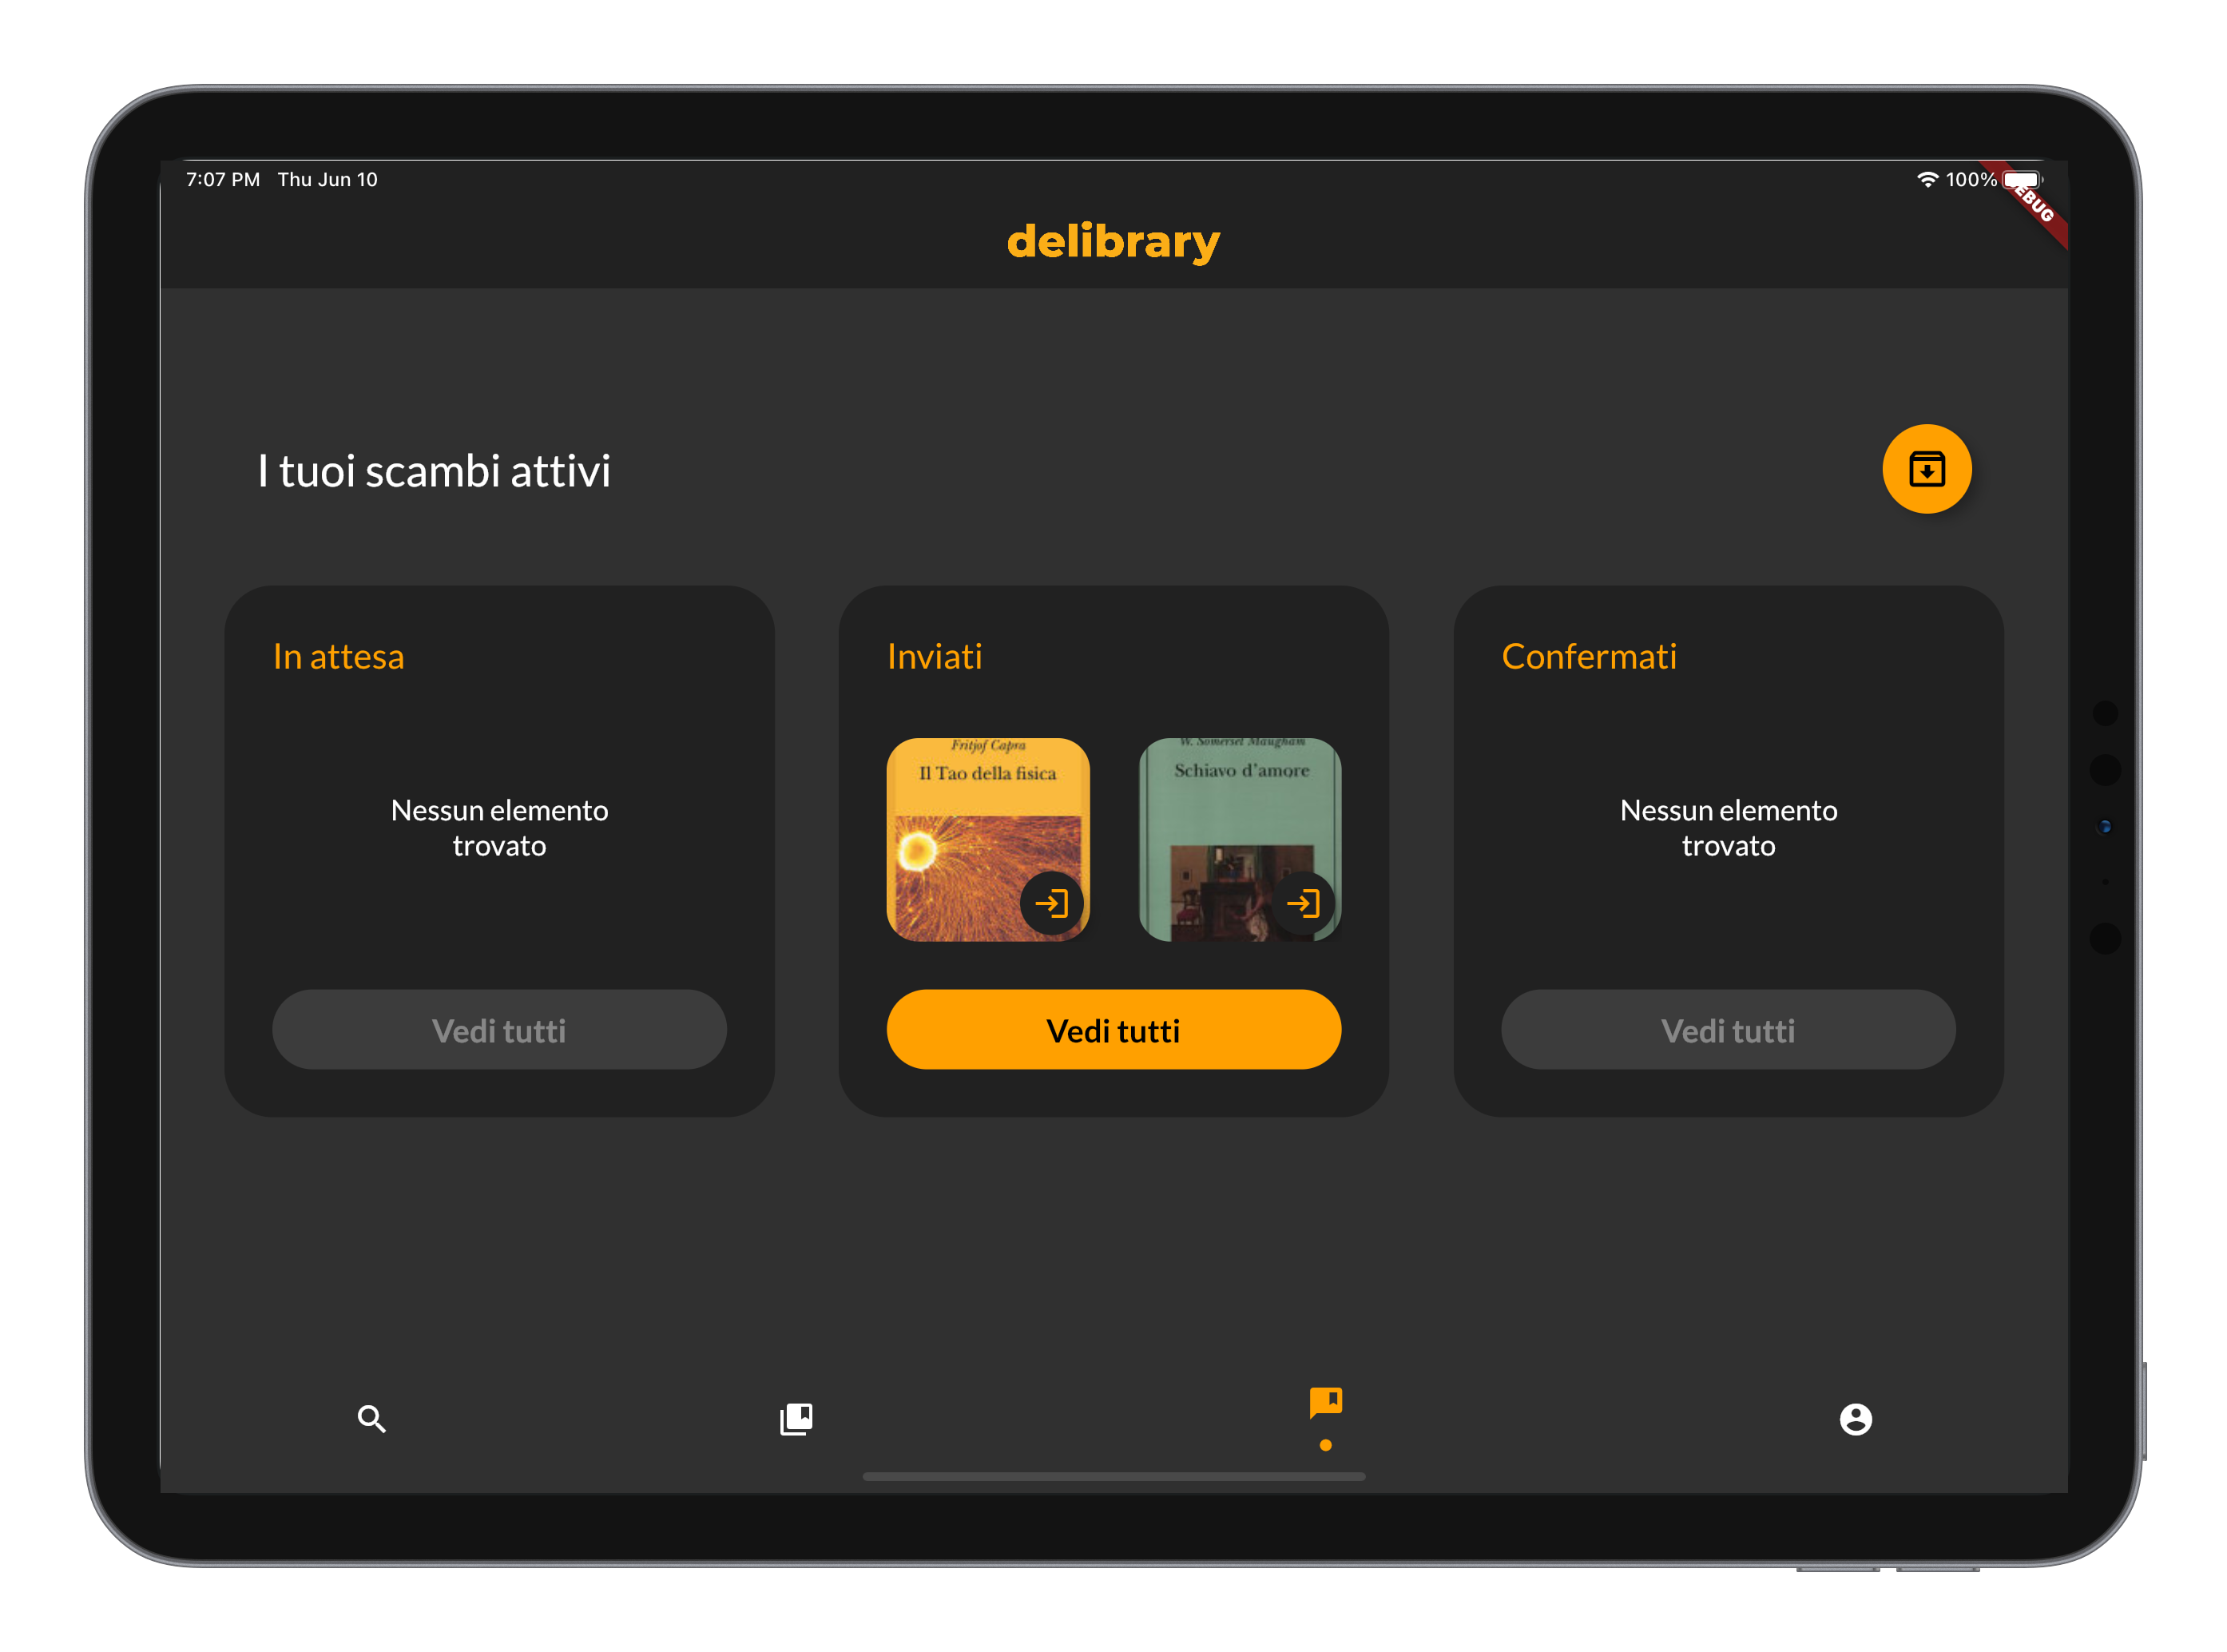
\includegraphics[width=0.65\textwidth]{screens/mock/tablet-landscape/exchanges.png}
            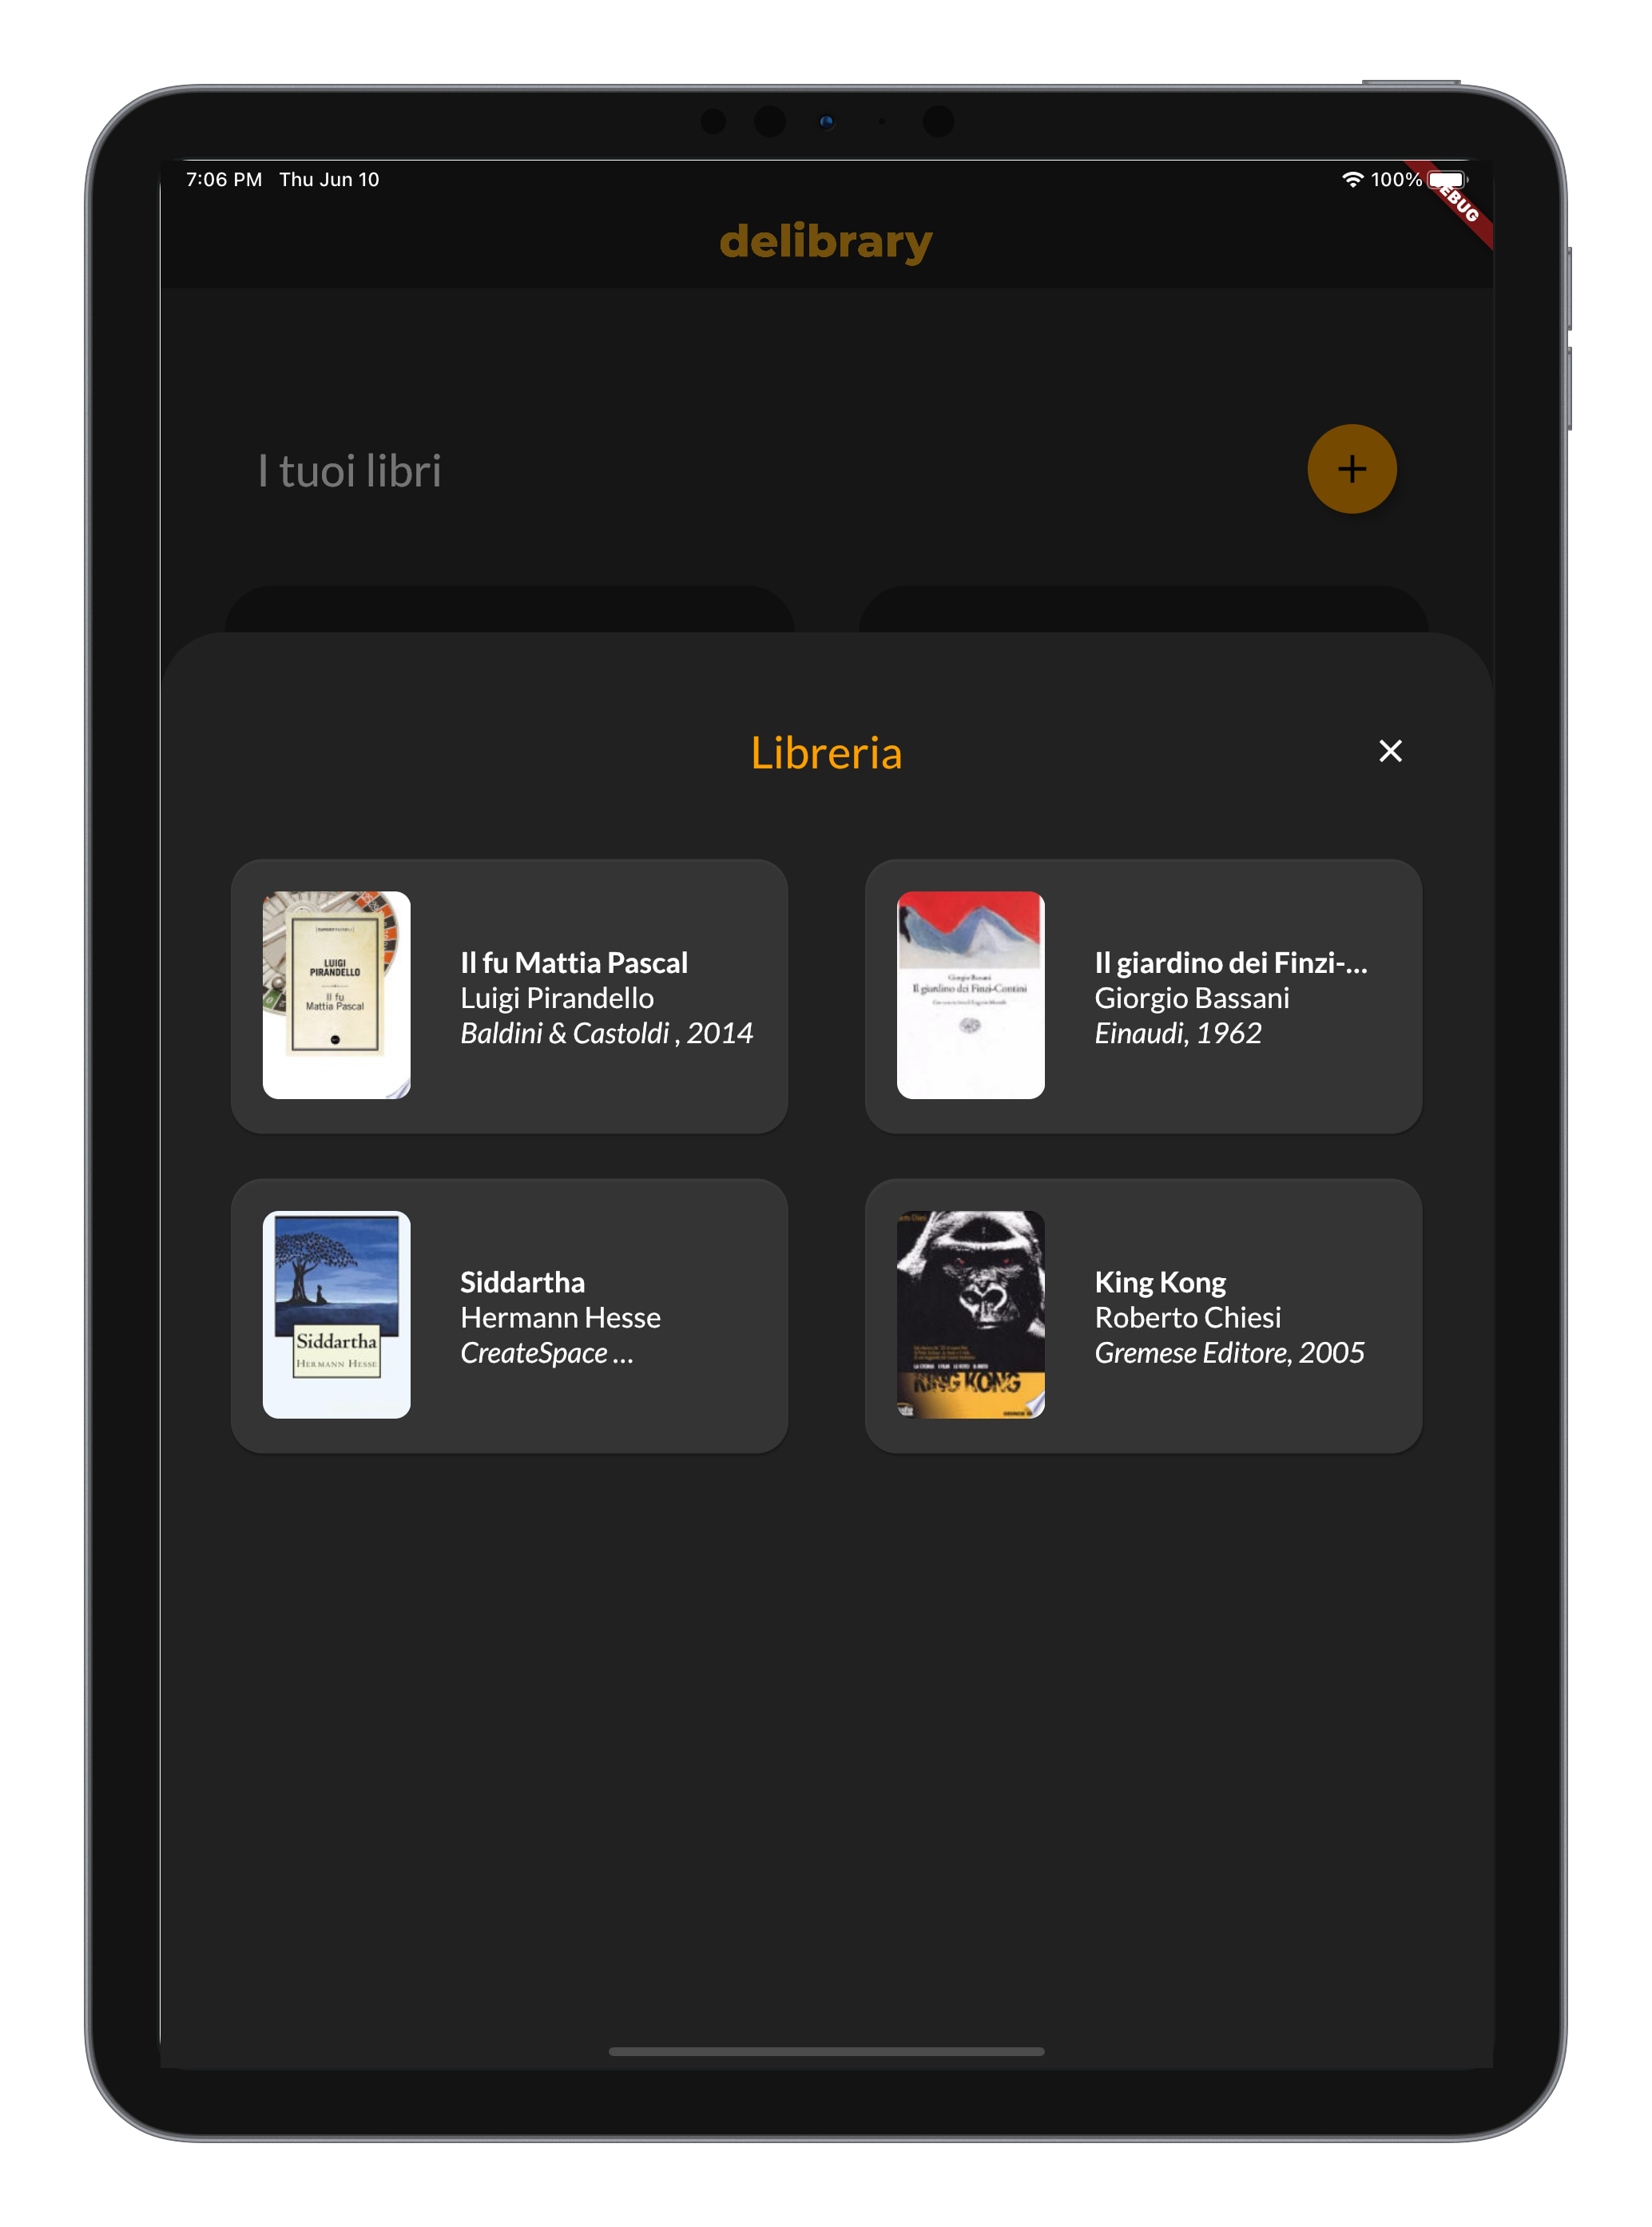
\includegraphics[width=0.45\textwidth]{screens/mock/tablet-portrait/library-expanded.png}
      }
      \makebox[\textwidth][c]{
            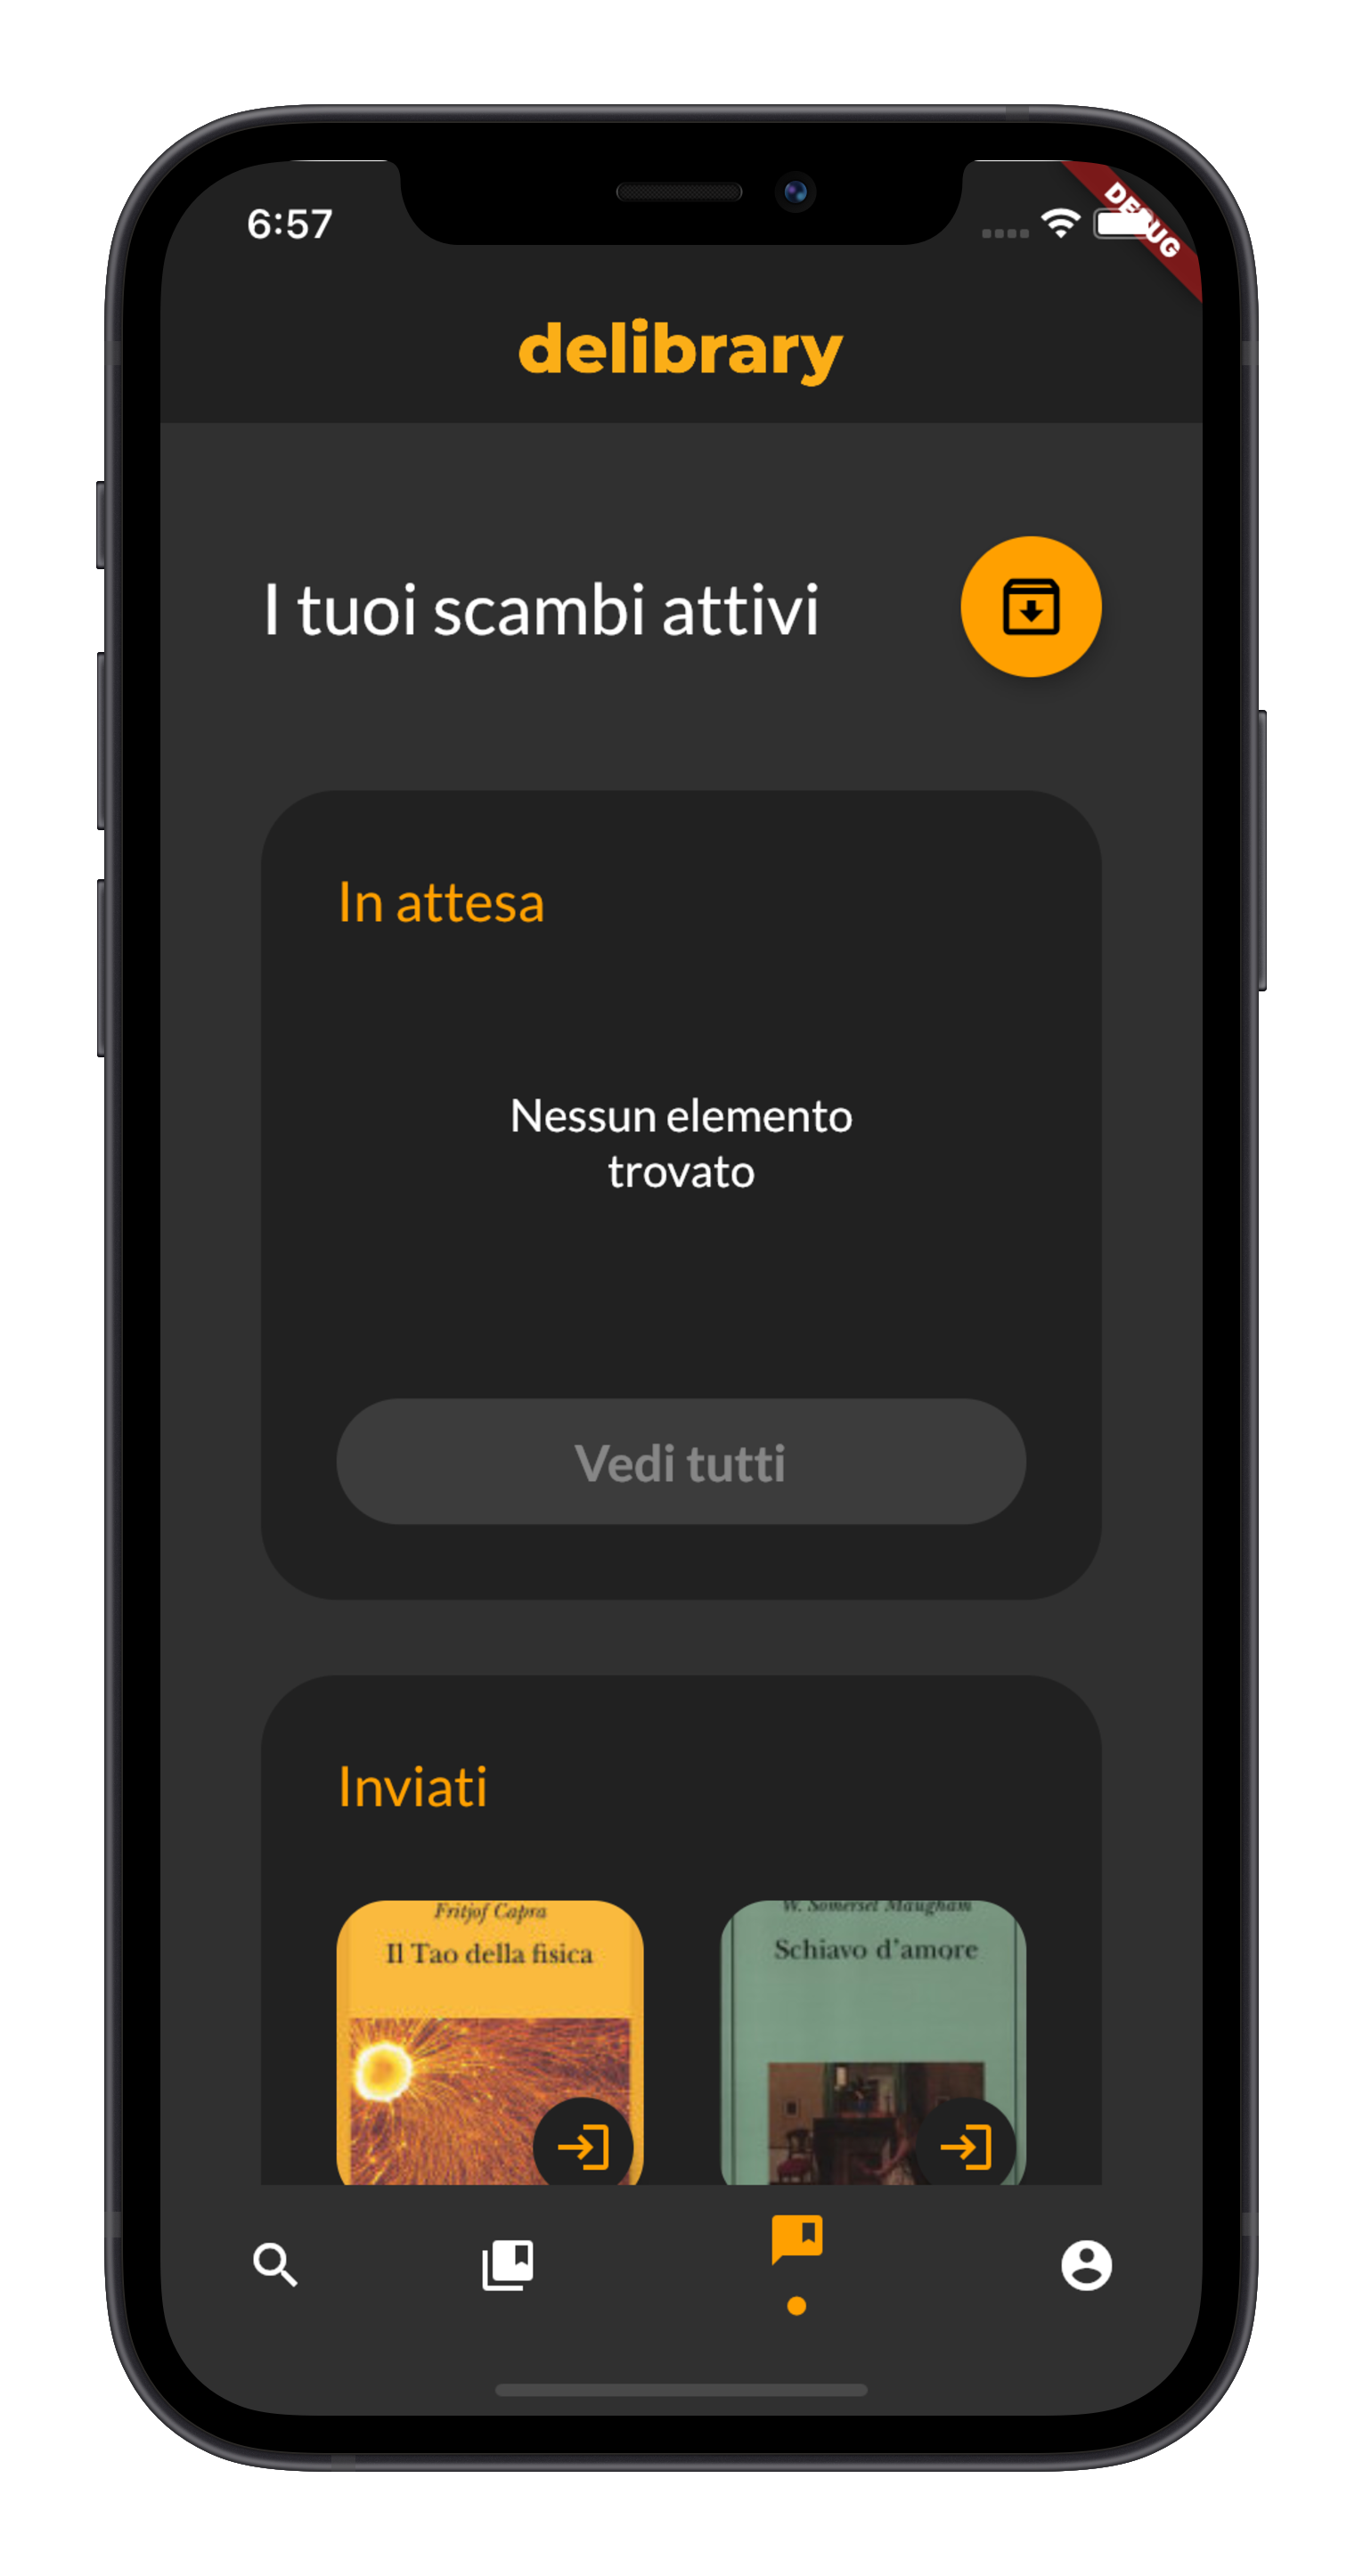
\includegraphics[width=0.35\textwidth]{screens/mock/smartphone/exchanges.png}
            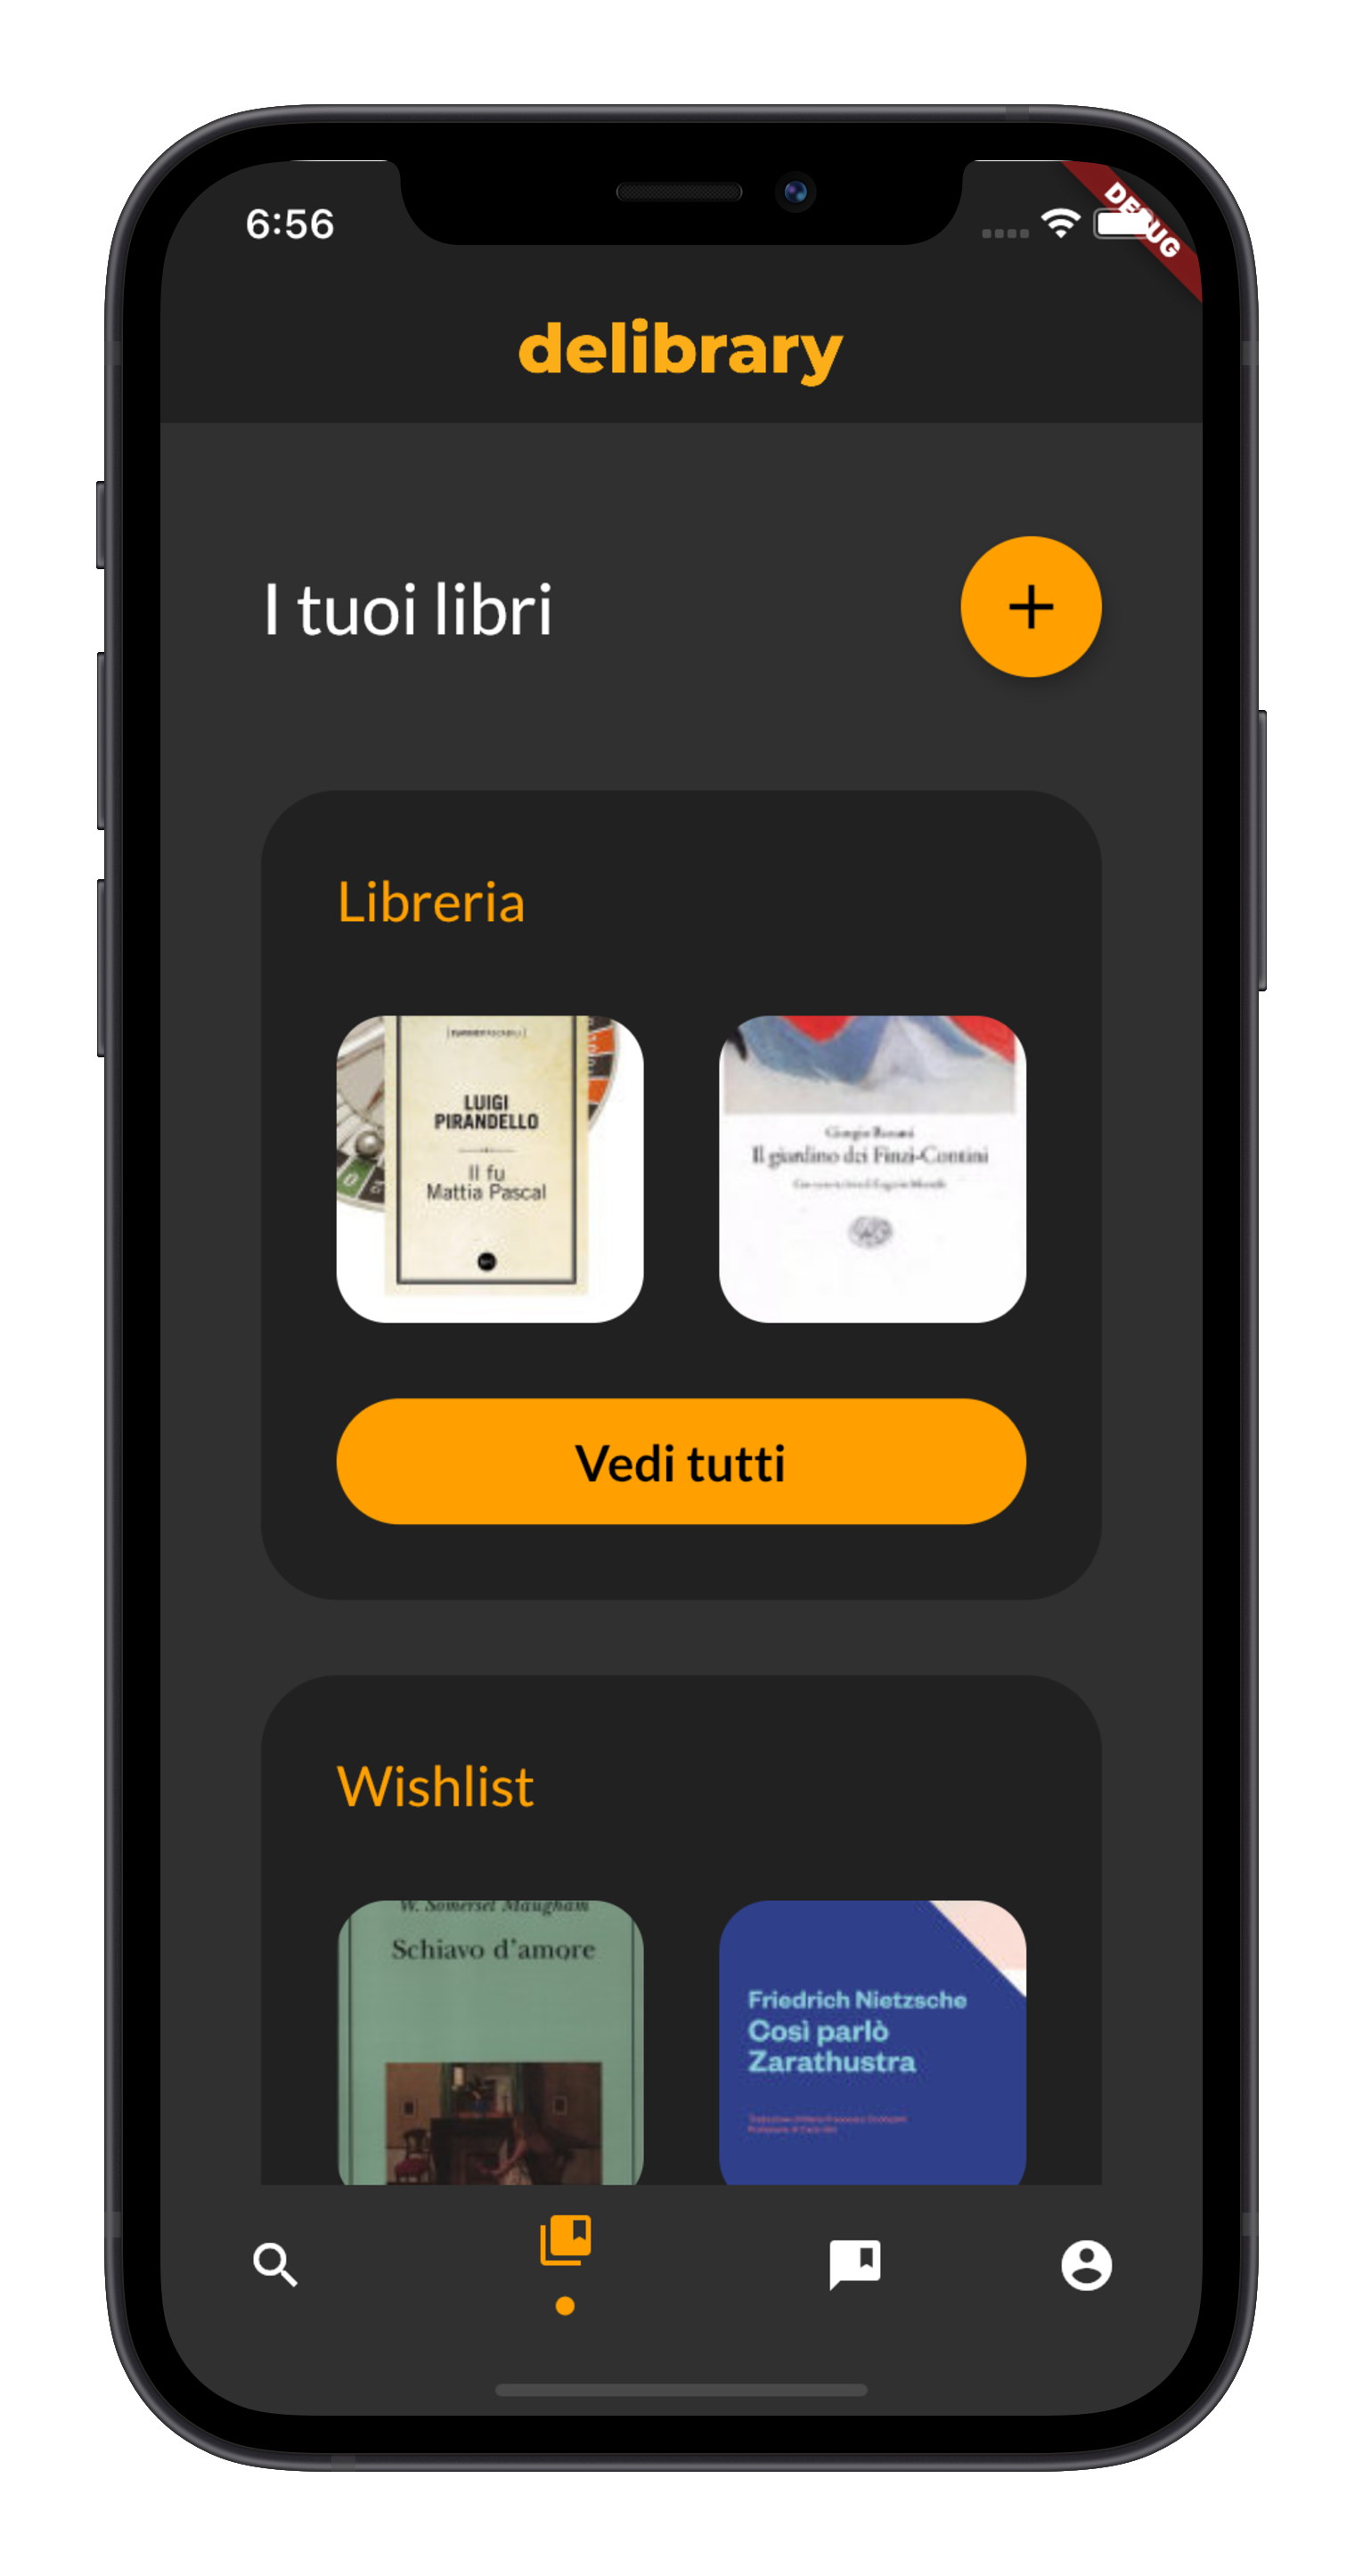
\includegraphics[width=0.35\textwidth]{screens/mock/smartphone/library.png}
            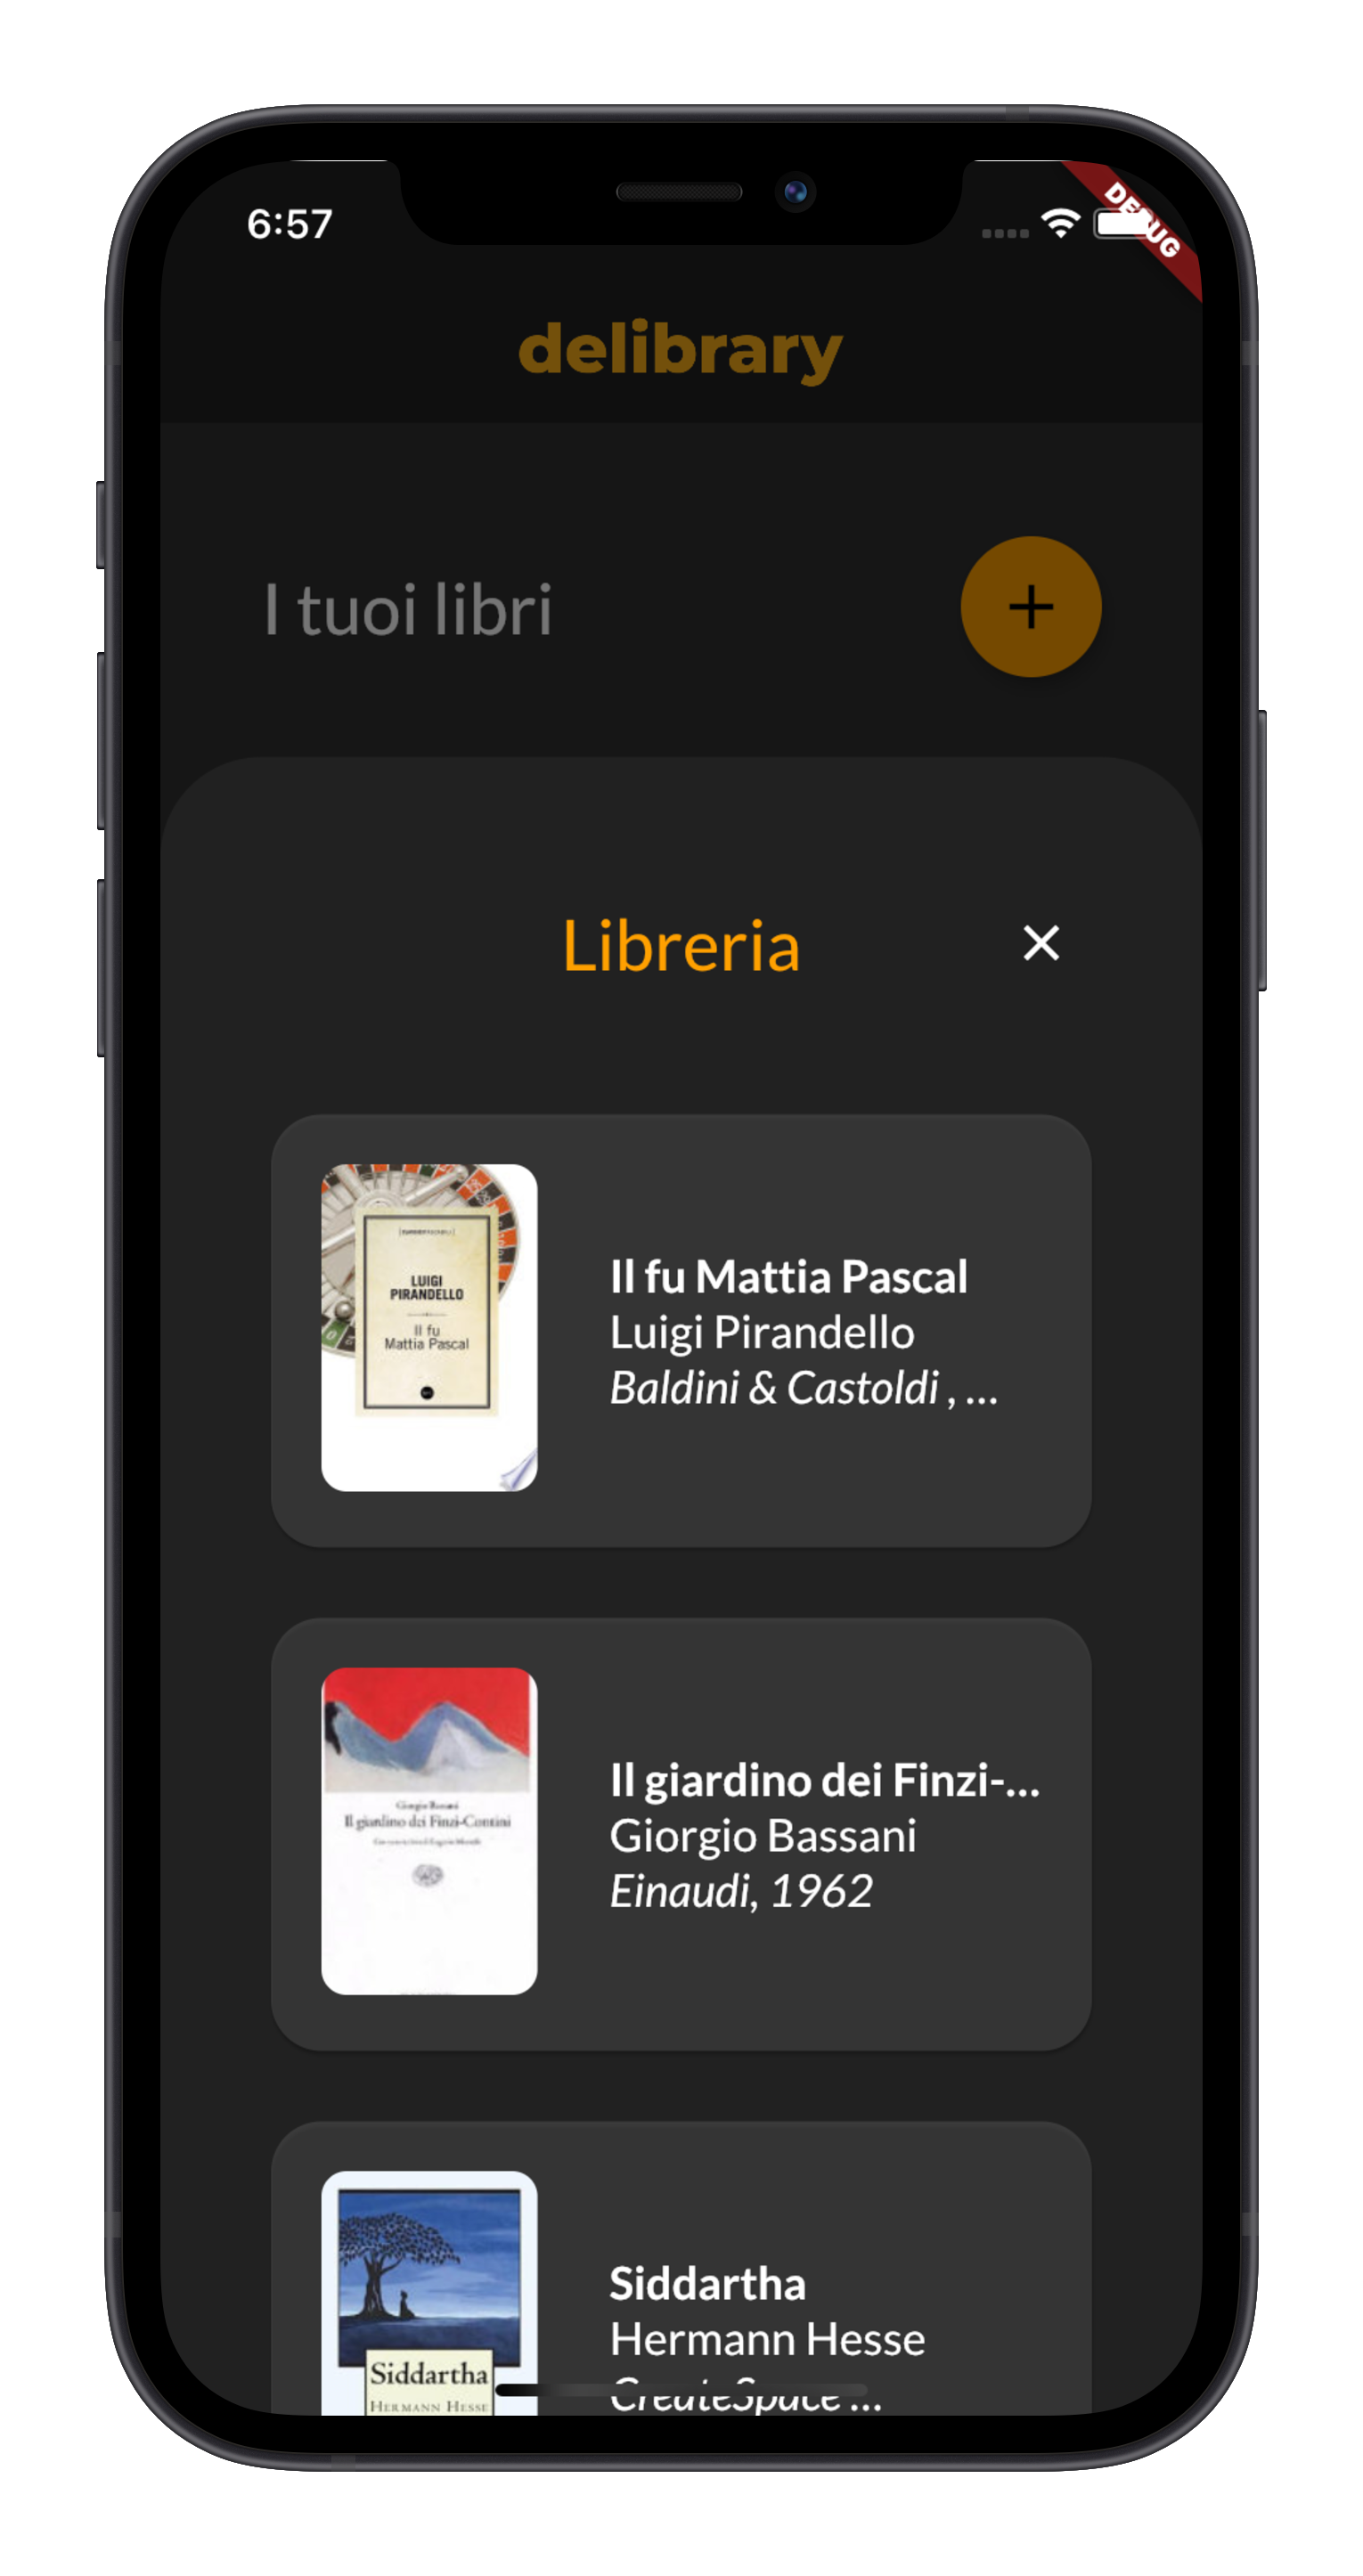
\includegraphics[width=0.35\textwidth]{screens/mock/smartphone/library-expanded.png}
      }
      \caption{Library and exchanges pages}
\end{figure}

\subsection{Book and Exchange Info}
Book and info pages will display all the information available and a list of buttons that correspond to the available actions.\\
Both the title and the description are limited to a fixed length, after which ellipsis are shown and the overflowed text can be seen with a tap.

\begin{figure}[H]
      \centering
      \makebox[\textwidth][c]{
            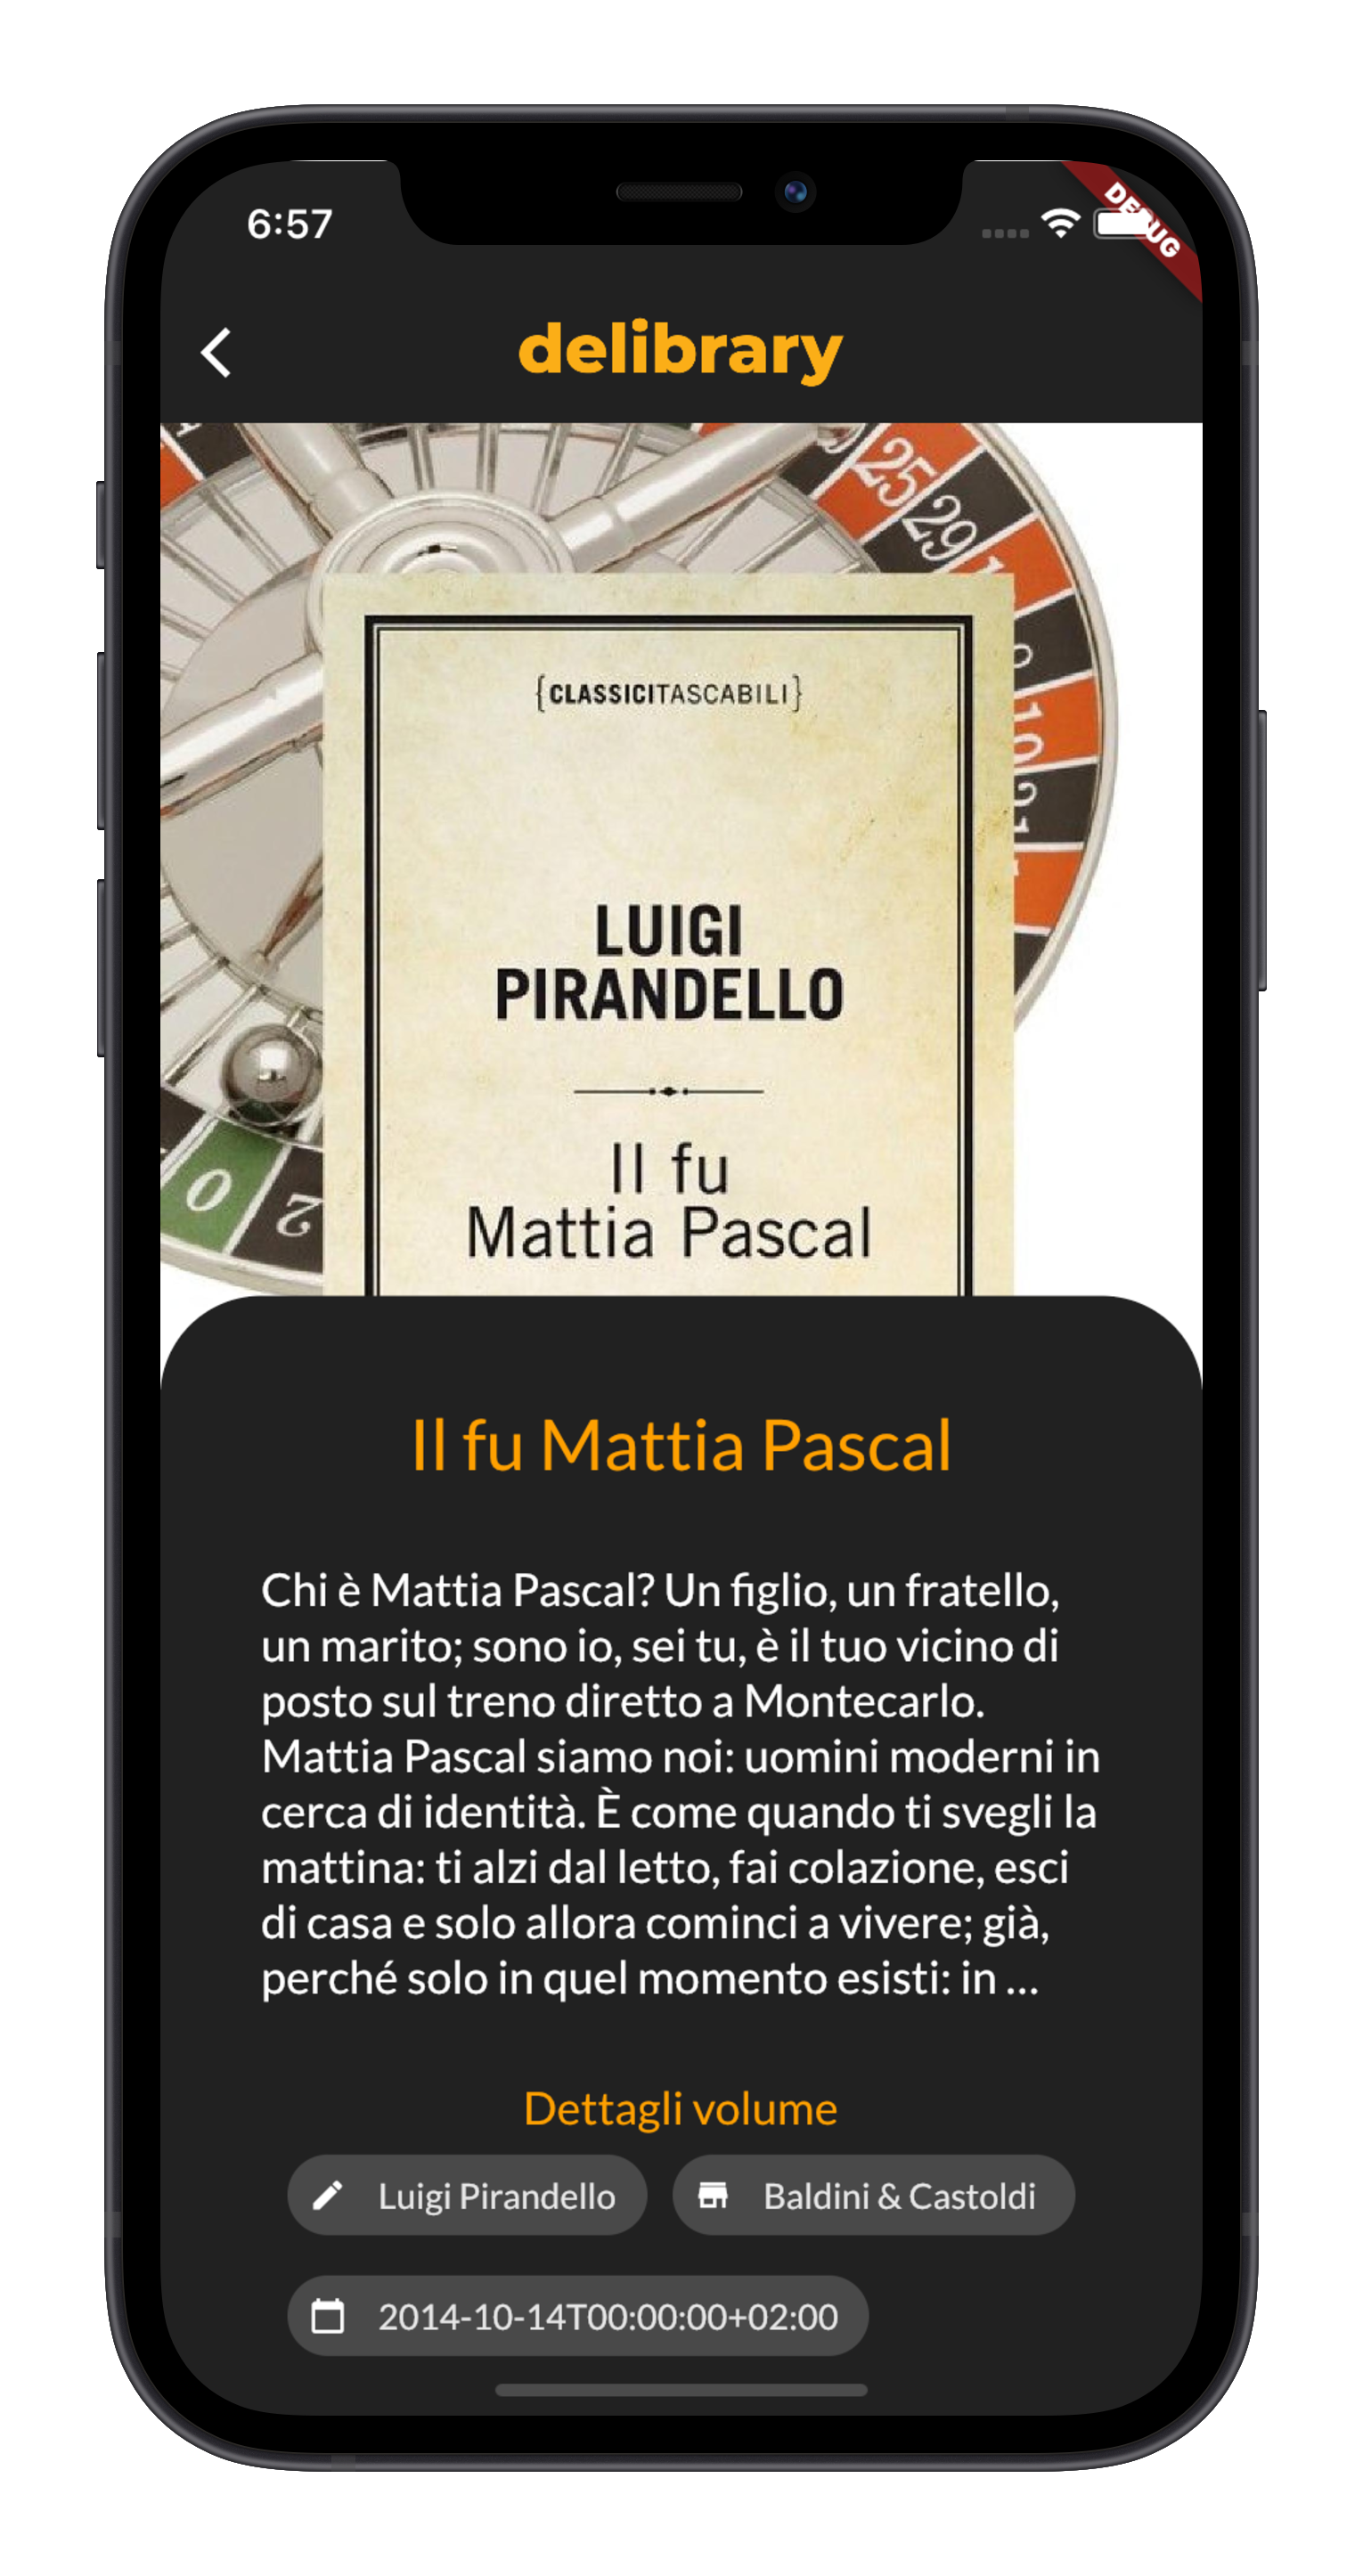
\includegraphics[width=0.35\textwidth]{screens/mock/smartphone/book-info.png}
            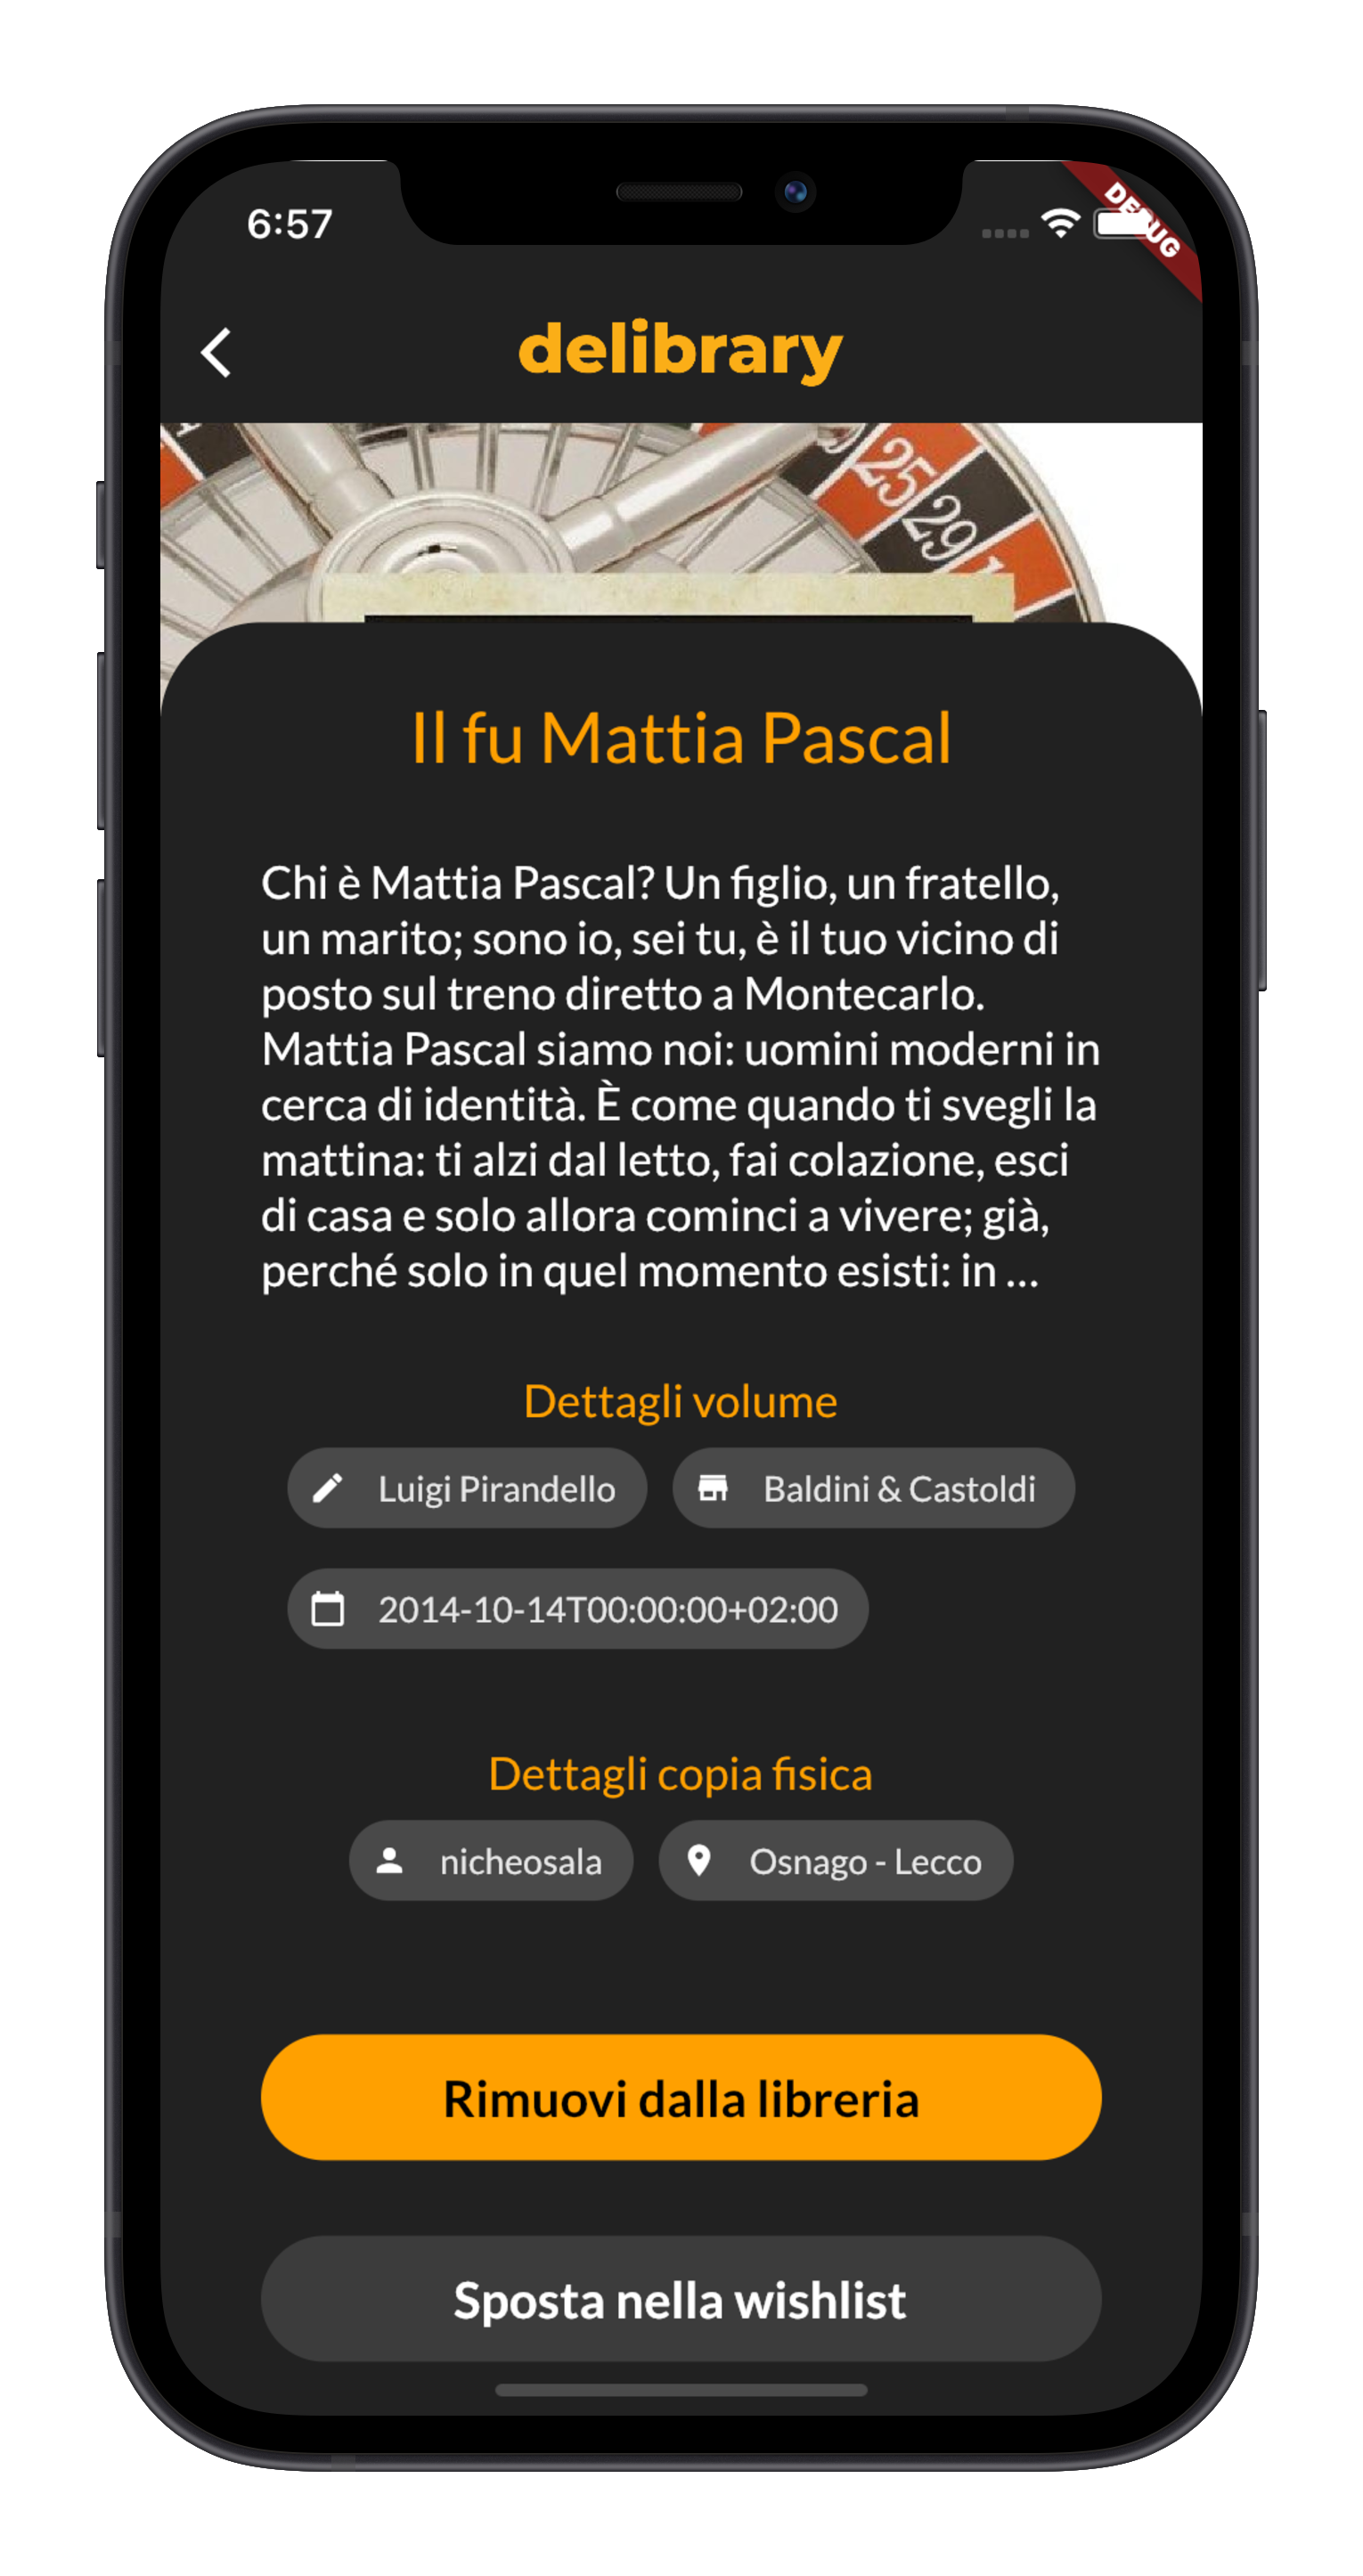
\includegraphics[width=0.35\textwidth]{screens/mock/smartphone/book-info-scrolled.png}
            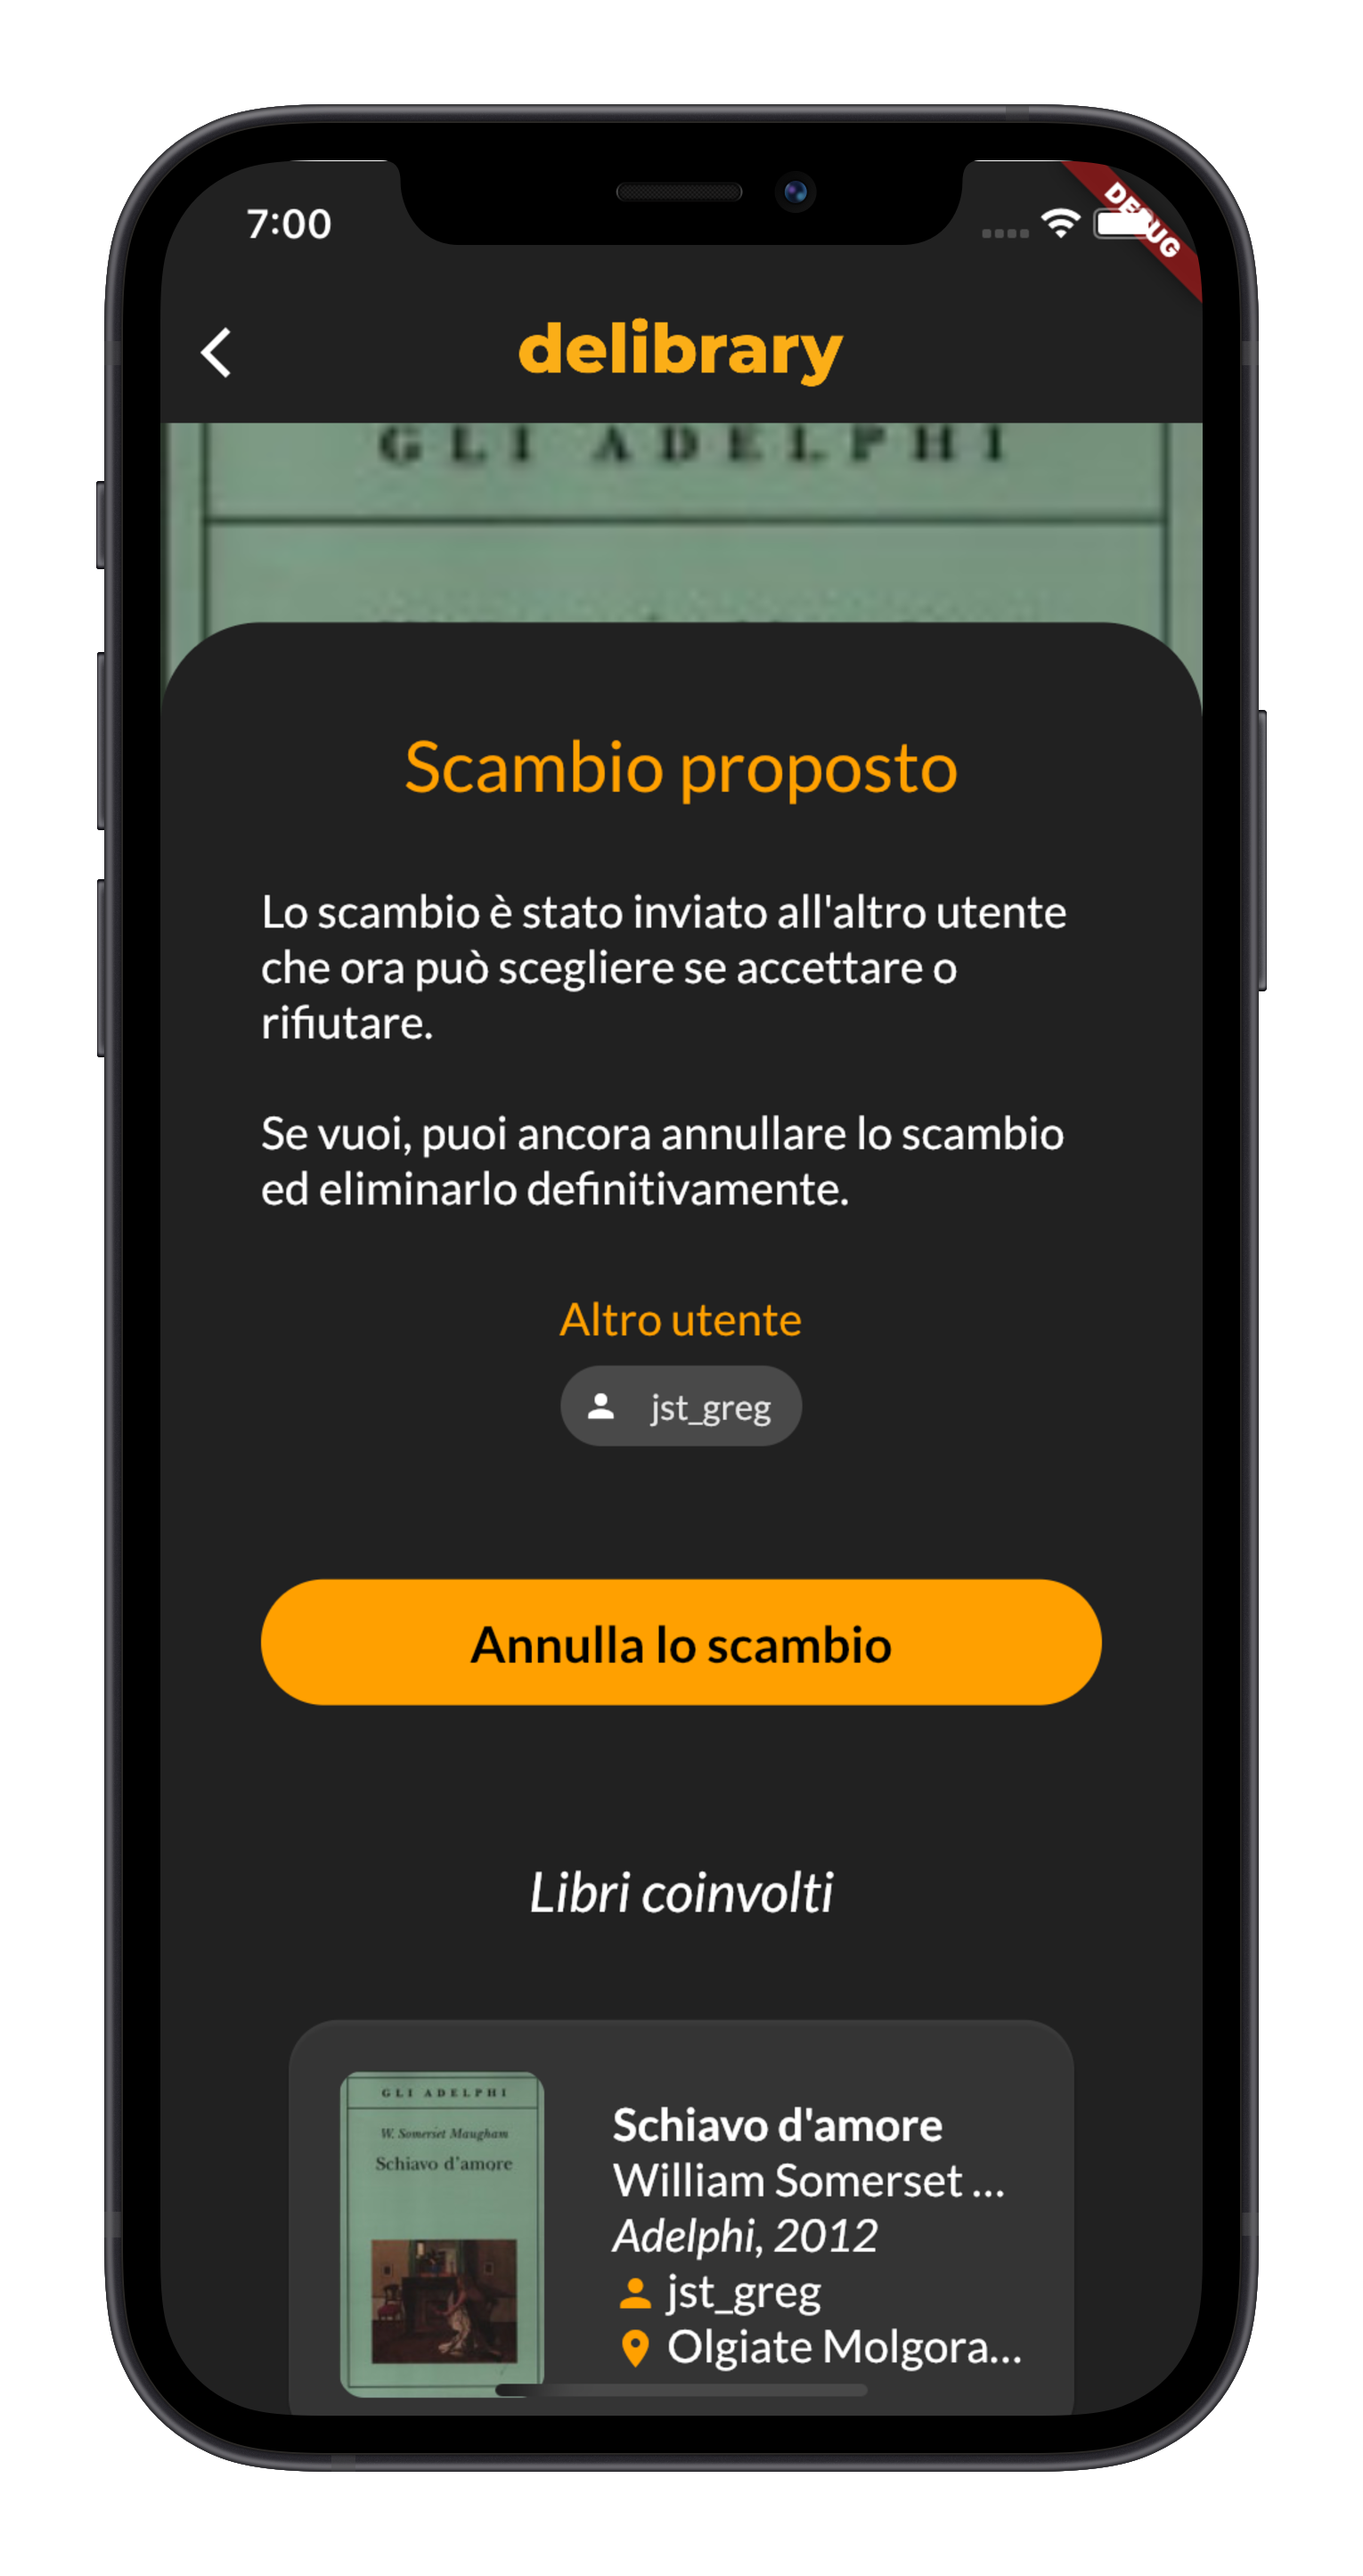
\includegraphics[width=0.35\textwidth]{screens/mock/smartphone/exchange-info-scrolled.png}
      }
      \makebox[\textwidth][c]{
            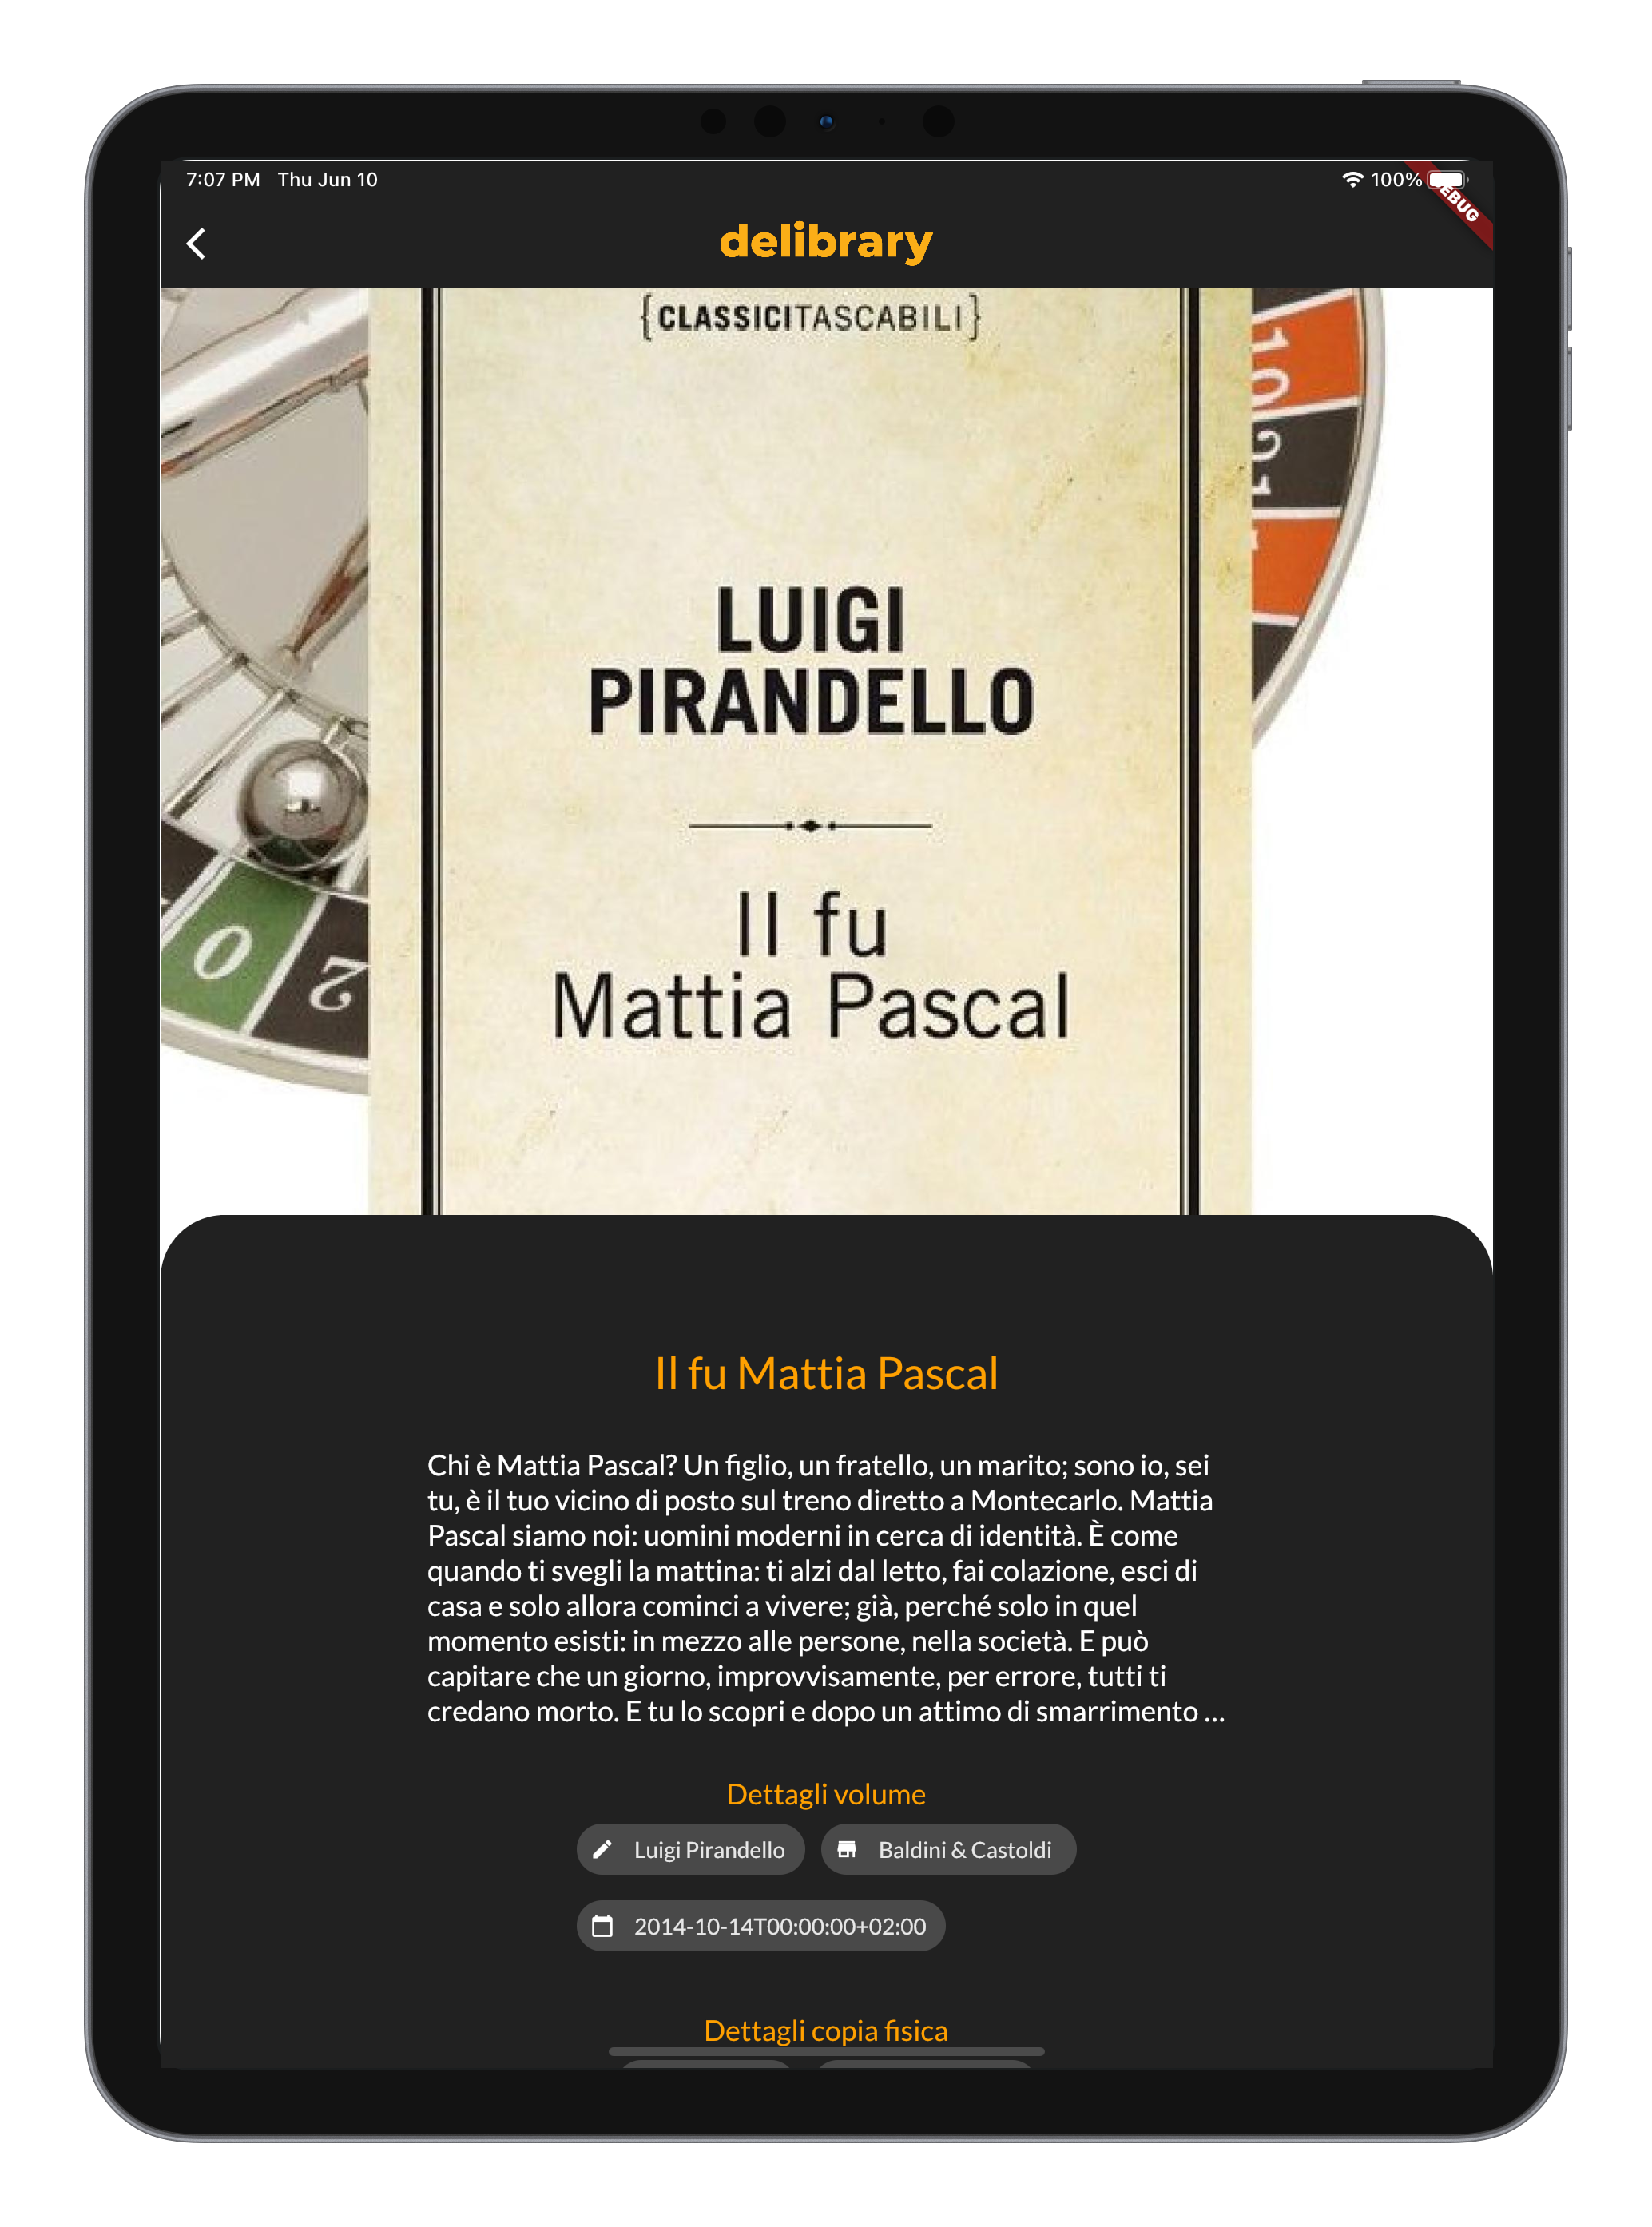
\includegraphics[width=0.45\textwidth]{screens/mock/tablet-portrait/book-info.png}
            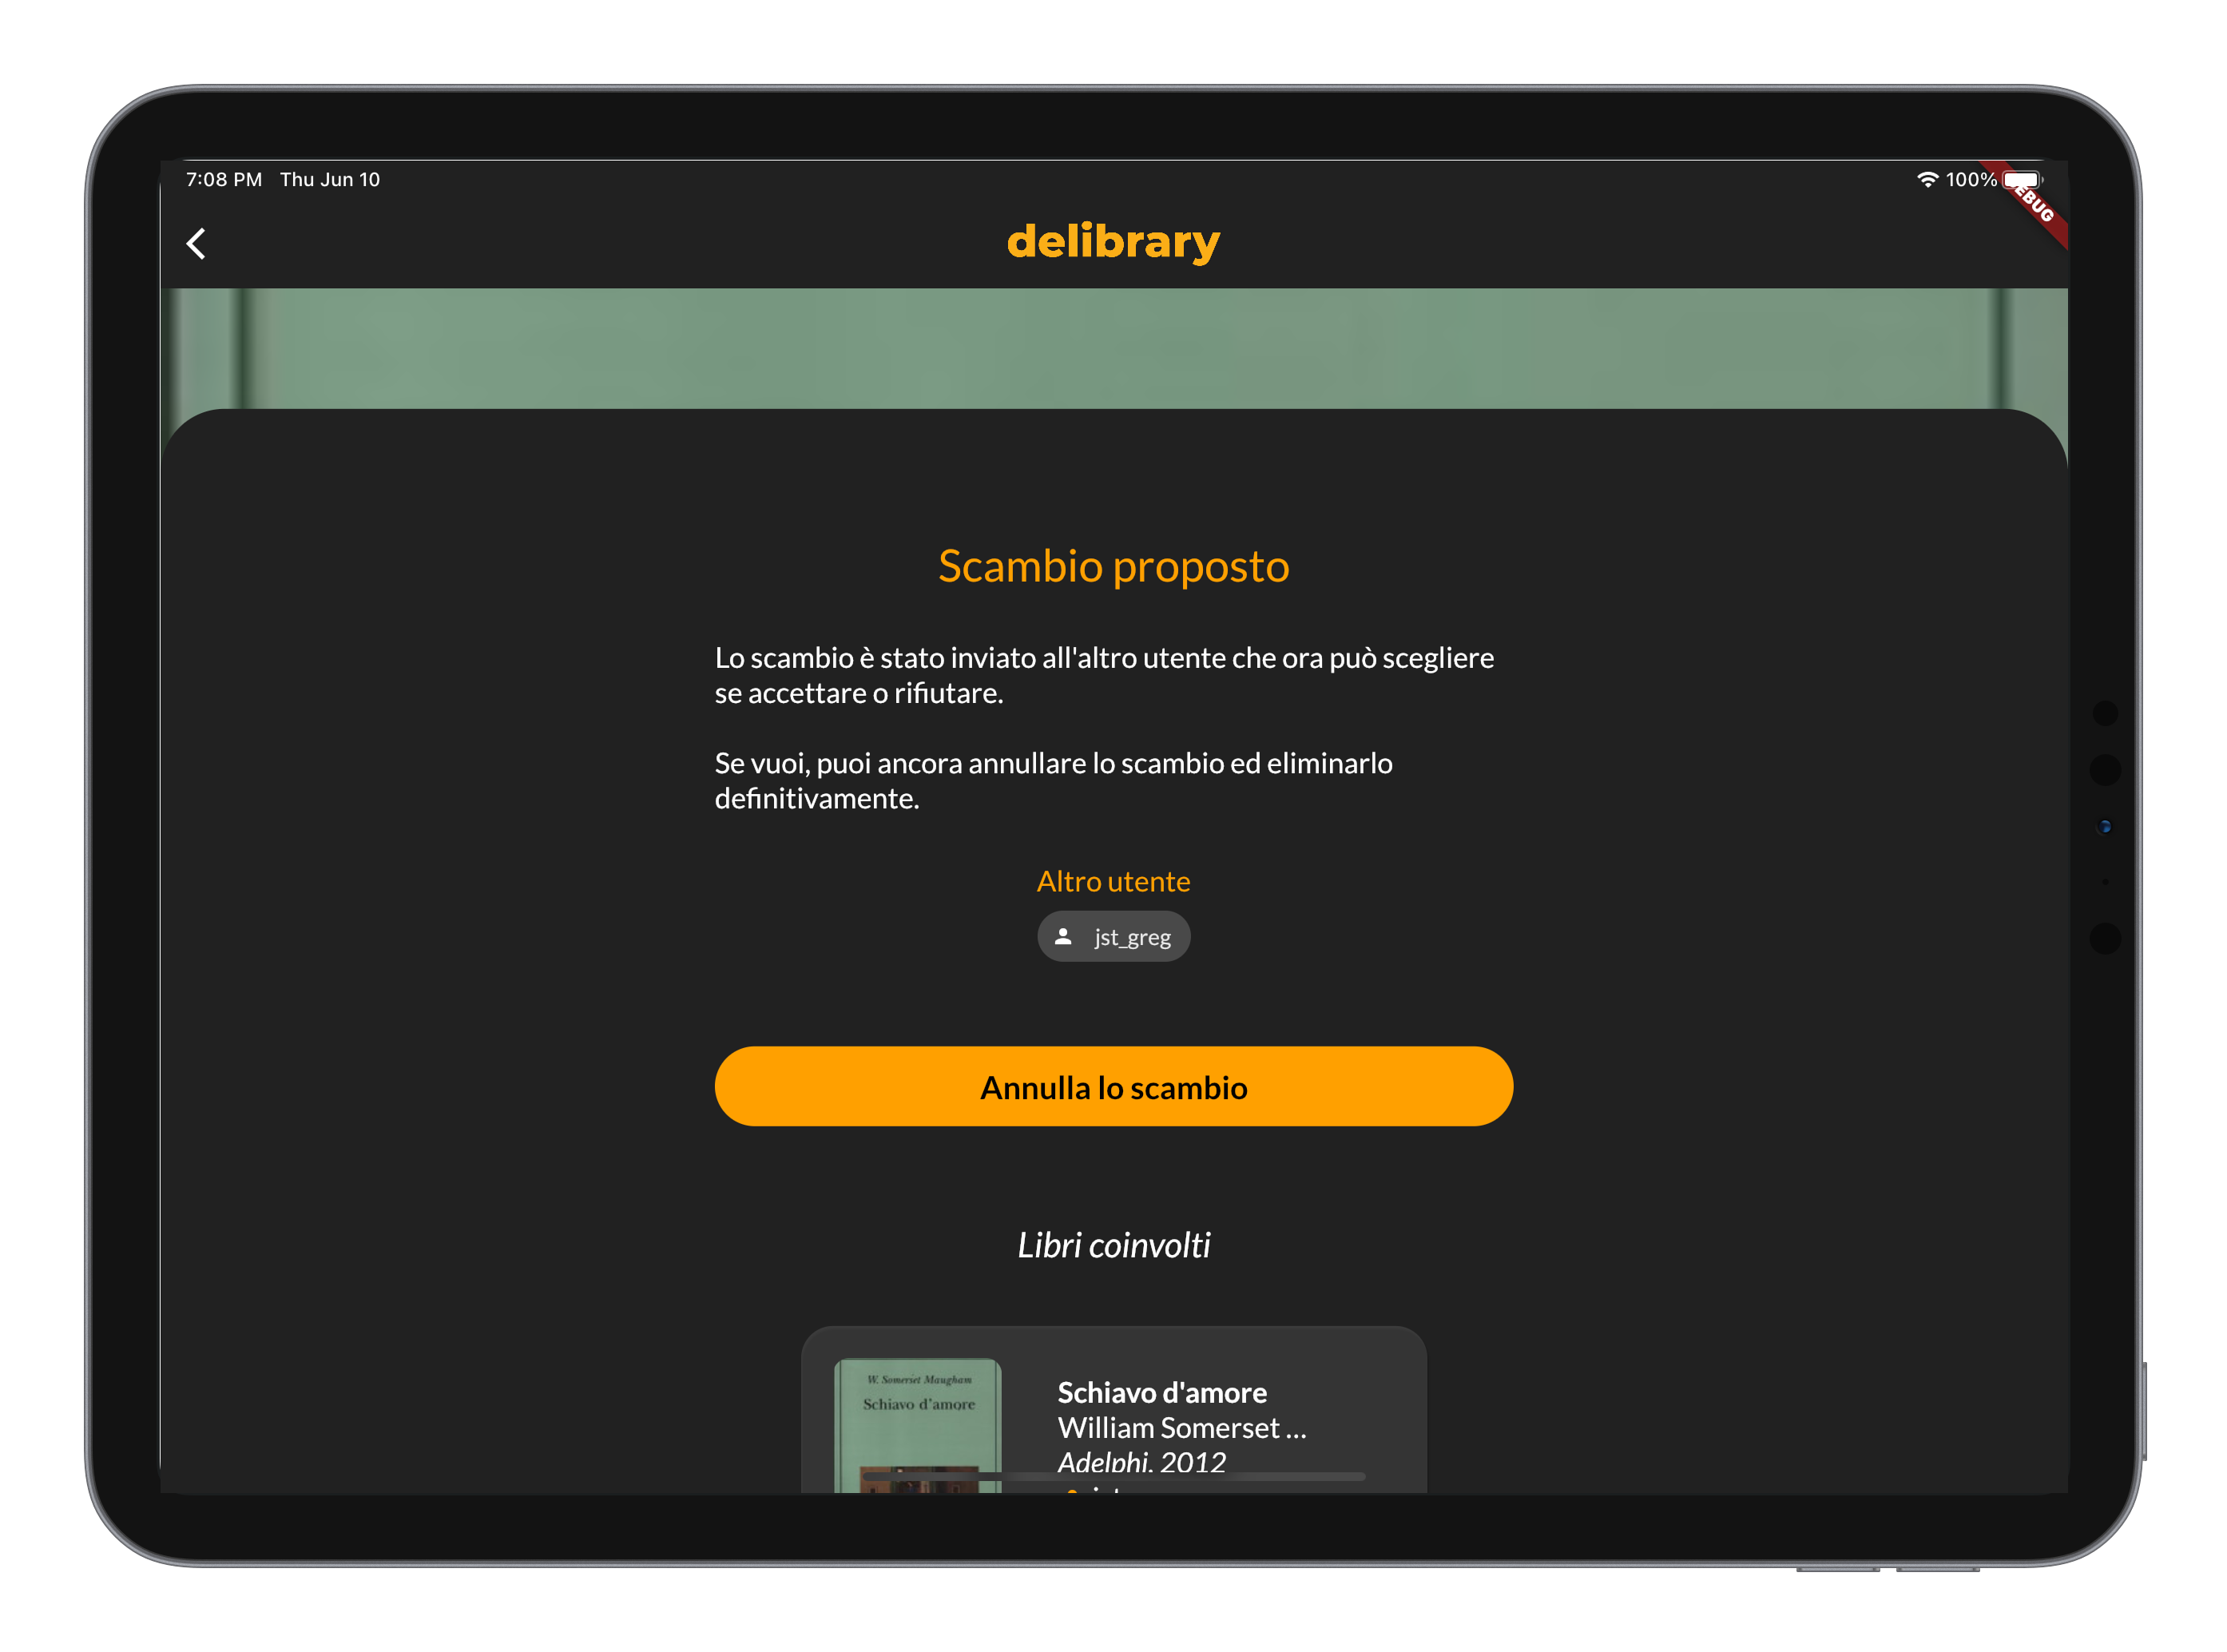
\includegraphics[width=0.65\textwidth]{screens/mock/tablet-landscape/exchange-info-scrolled.png}
      }
      \caption{Book and exchange info pages}
\end{figure}

\subsection{Profile}
Finally, each user has a profile page from which is able to edit their personal information and their password as well as log out from Delibrary.

\begin{figure}[H]
      \centering
      \makebox[\textwidth][c]{
            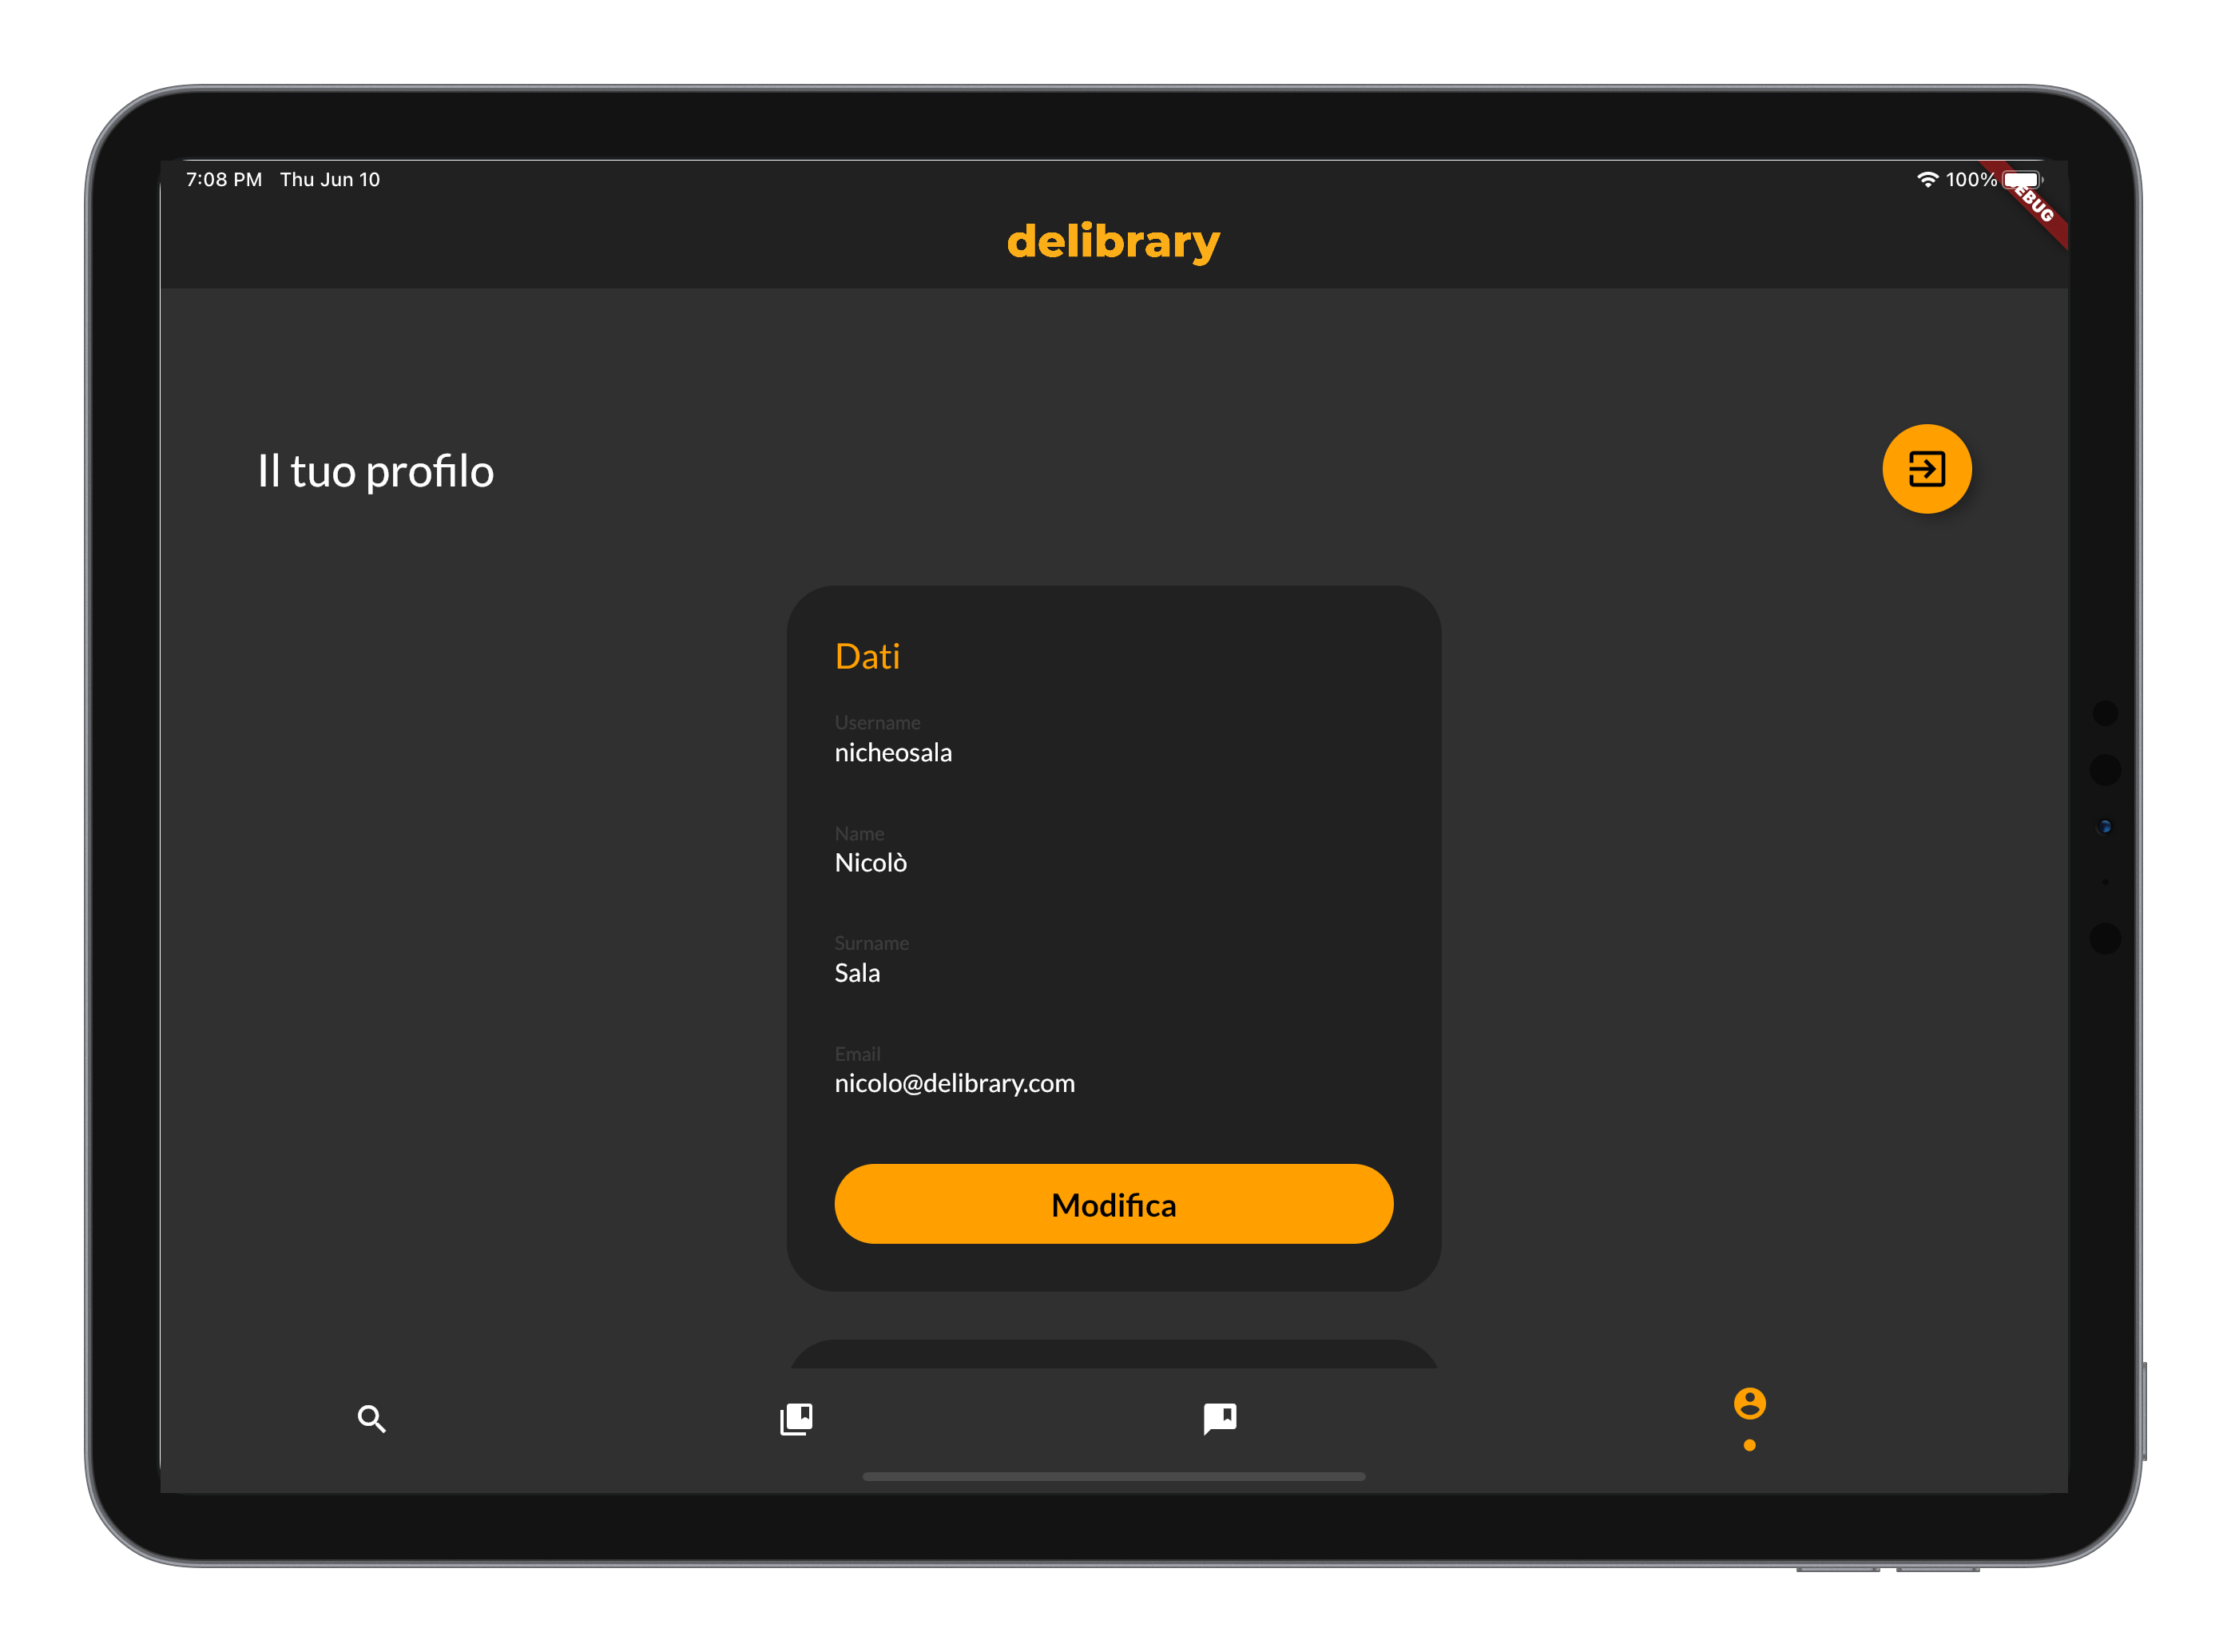
\includegraphics[width=0.75\textwidth]{screens/mock/tablet-landscape/profile.png}
            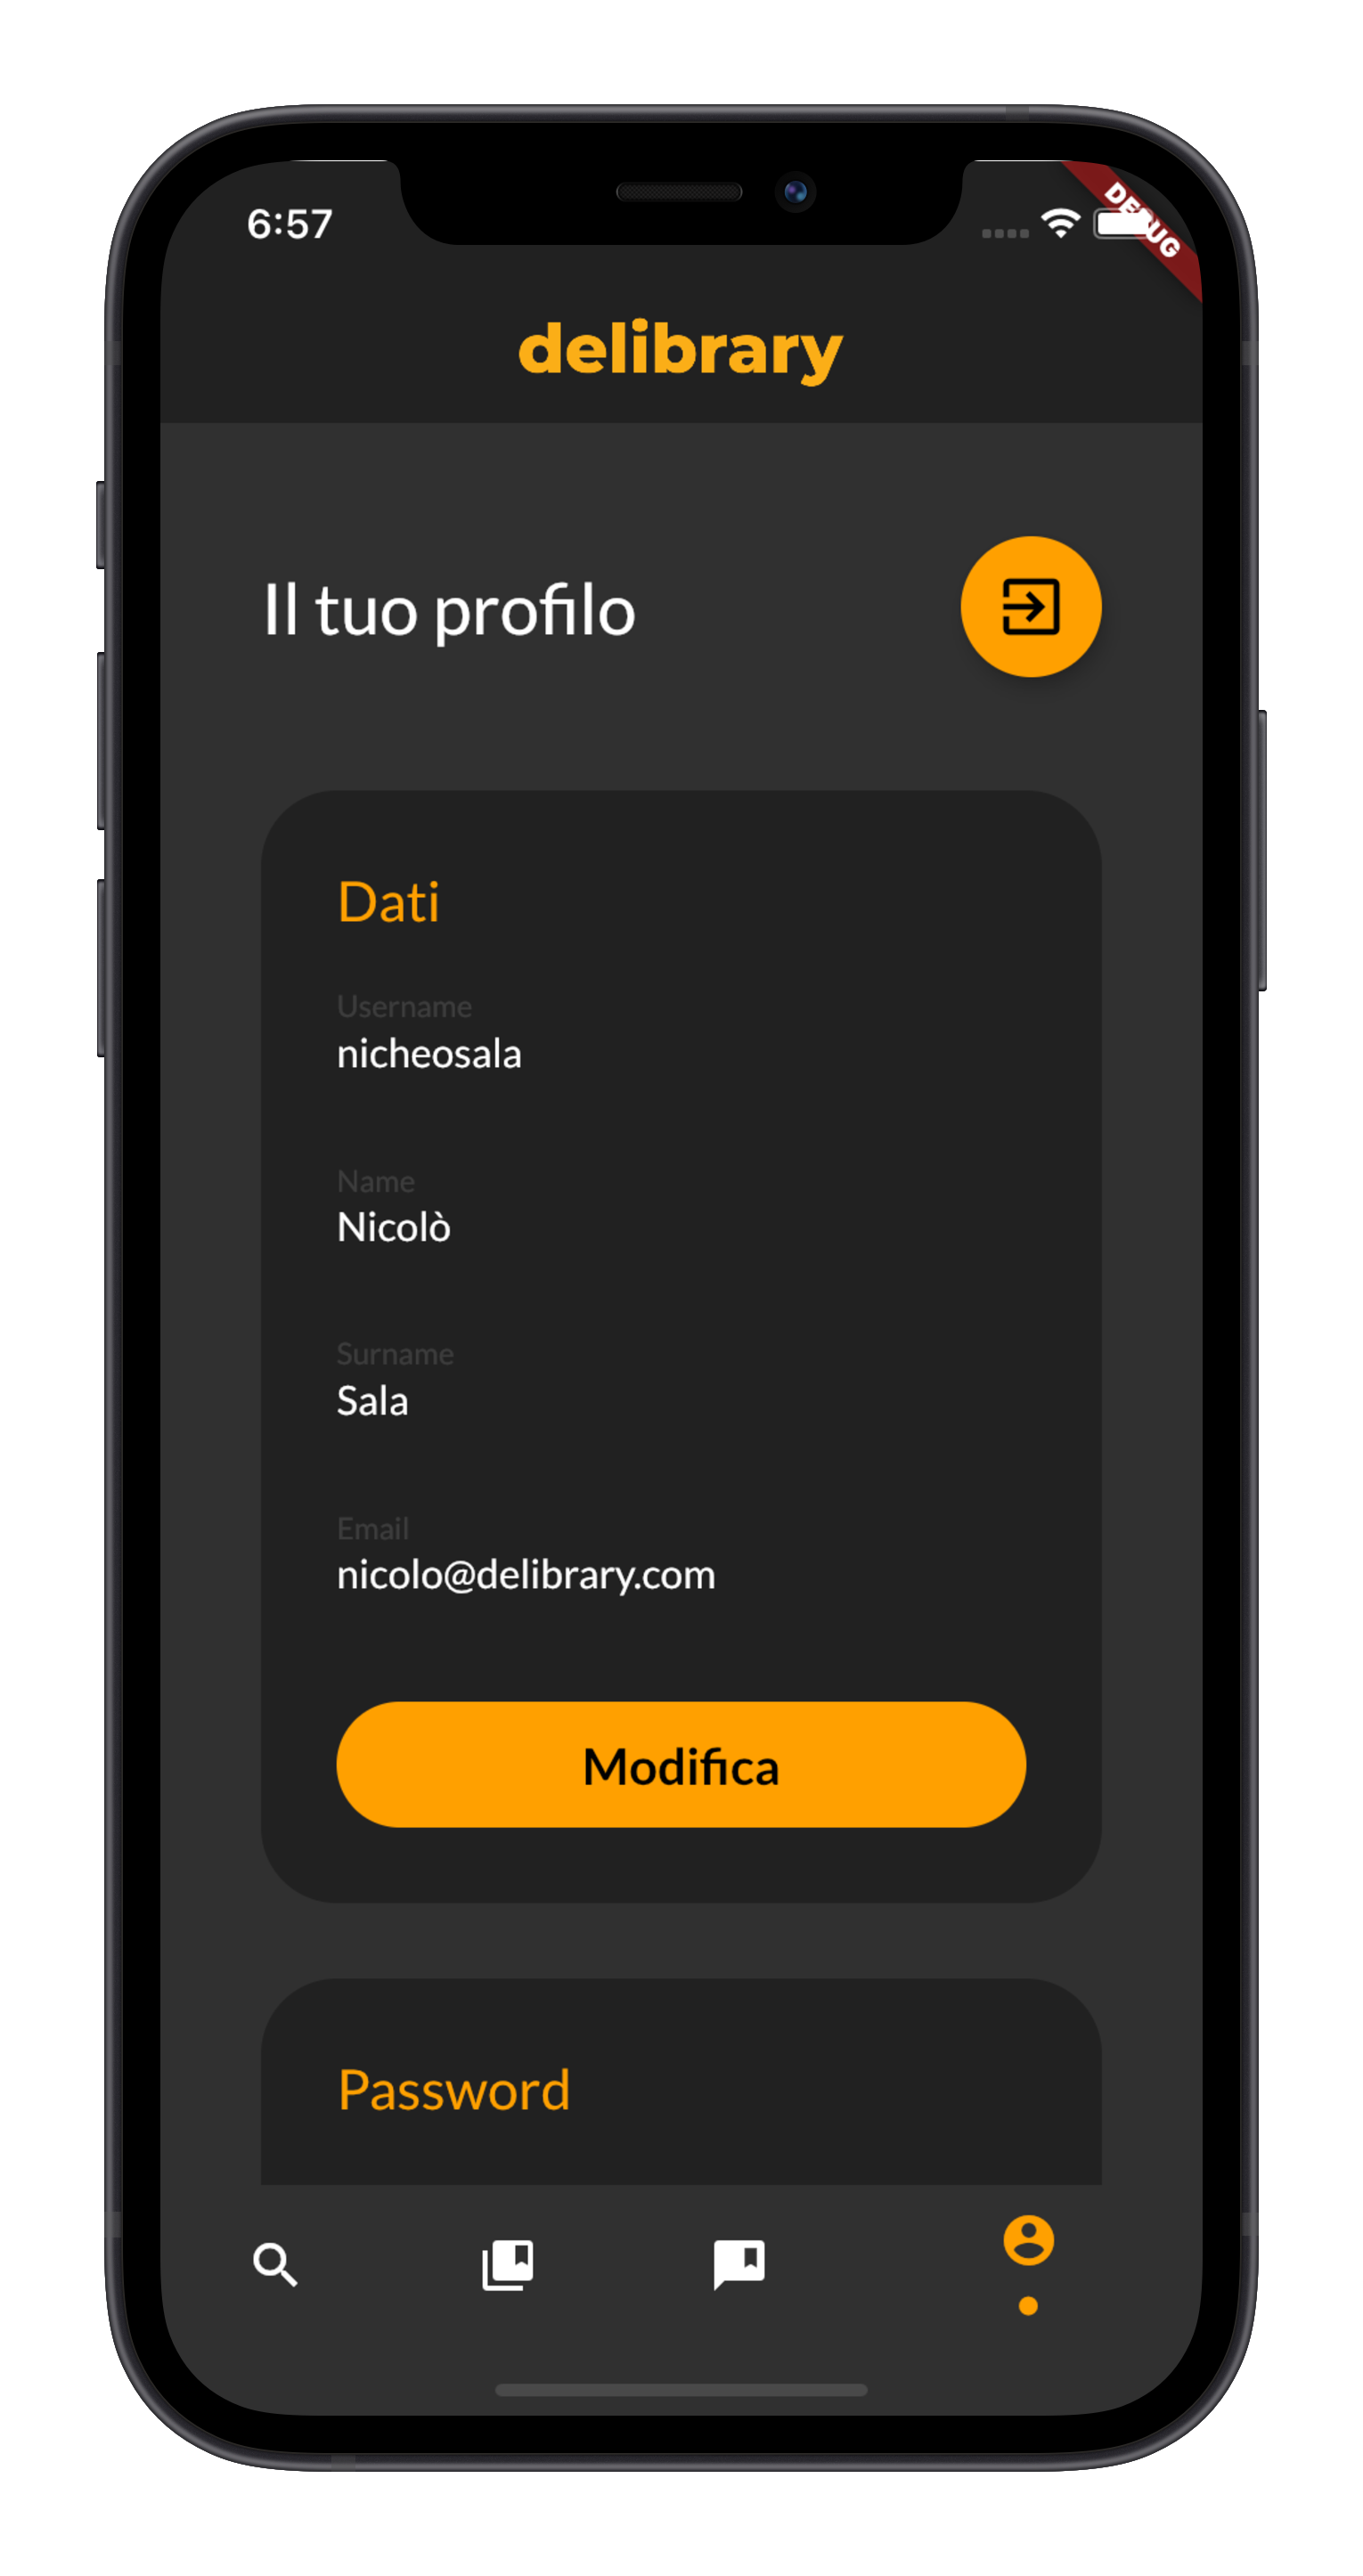
\includegraphics[width=0.34\textwidth]{screens/mock/smartphone/profile.png}
      }
      \makebox[\textwidth][c]{
            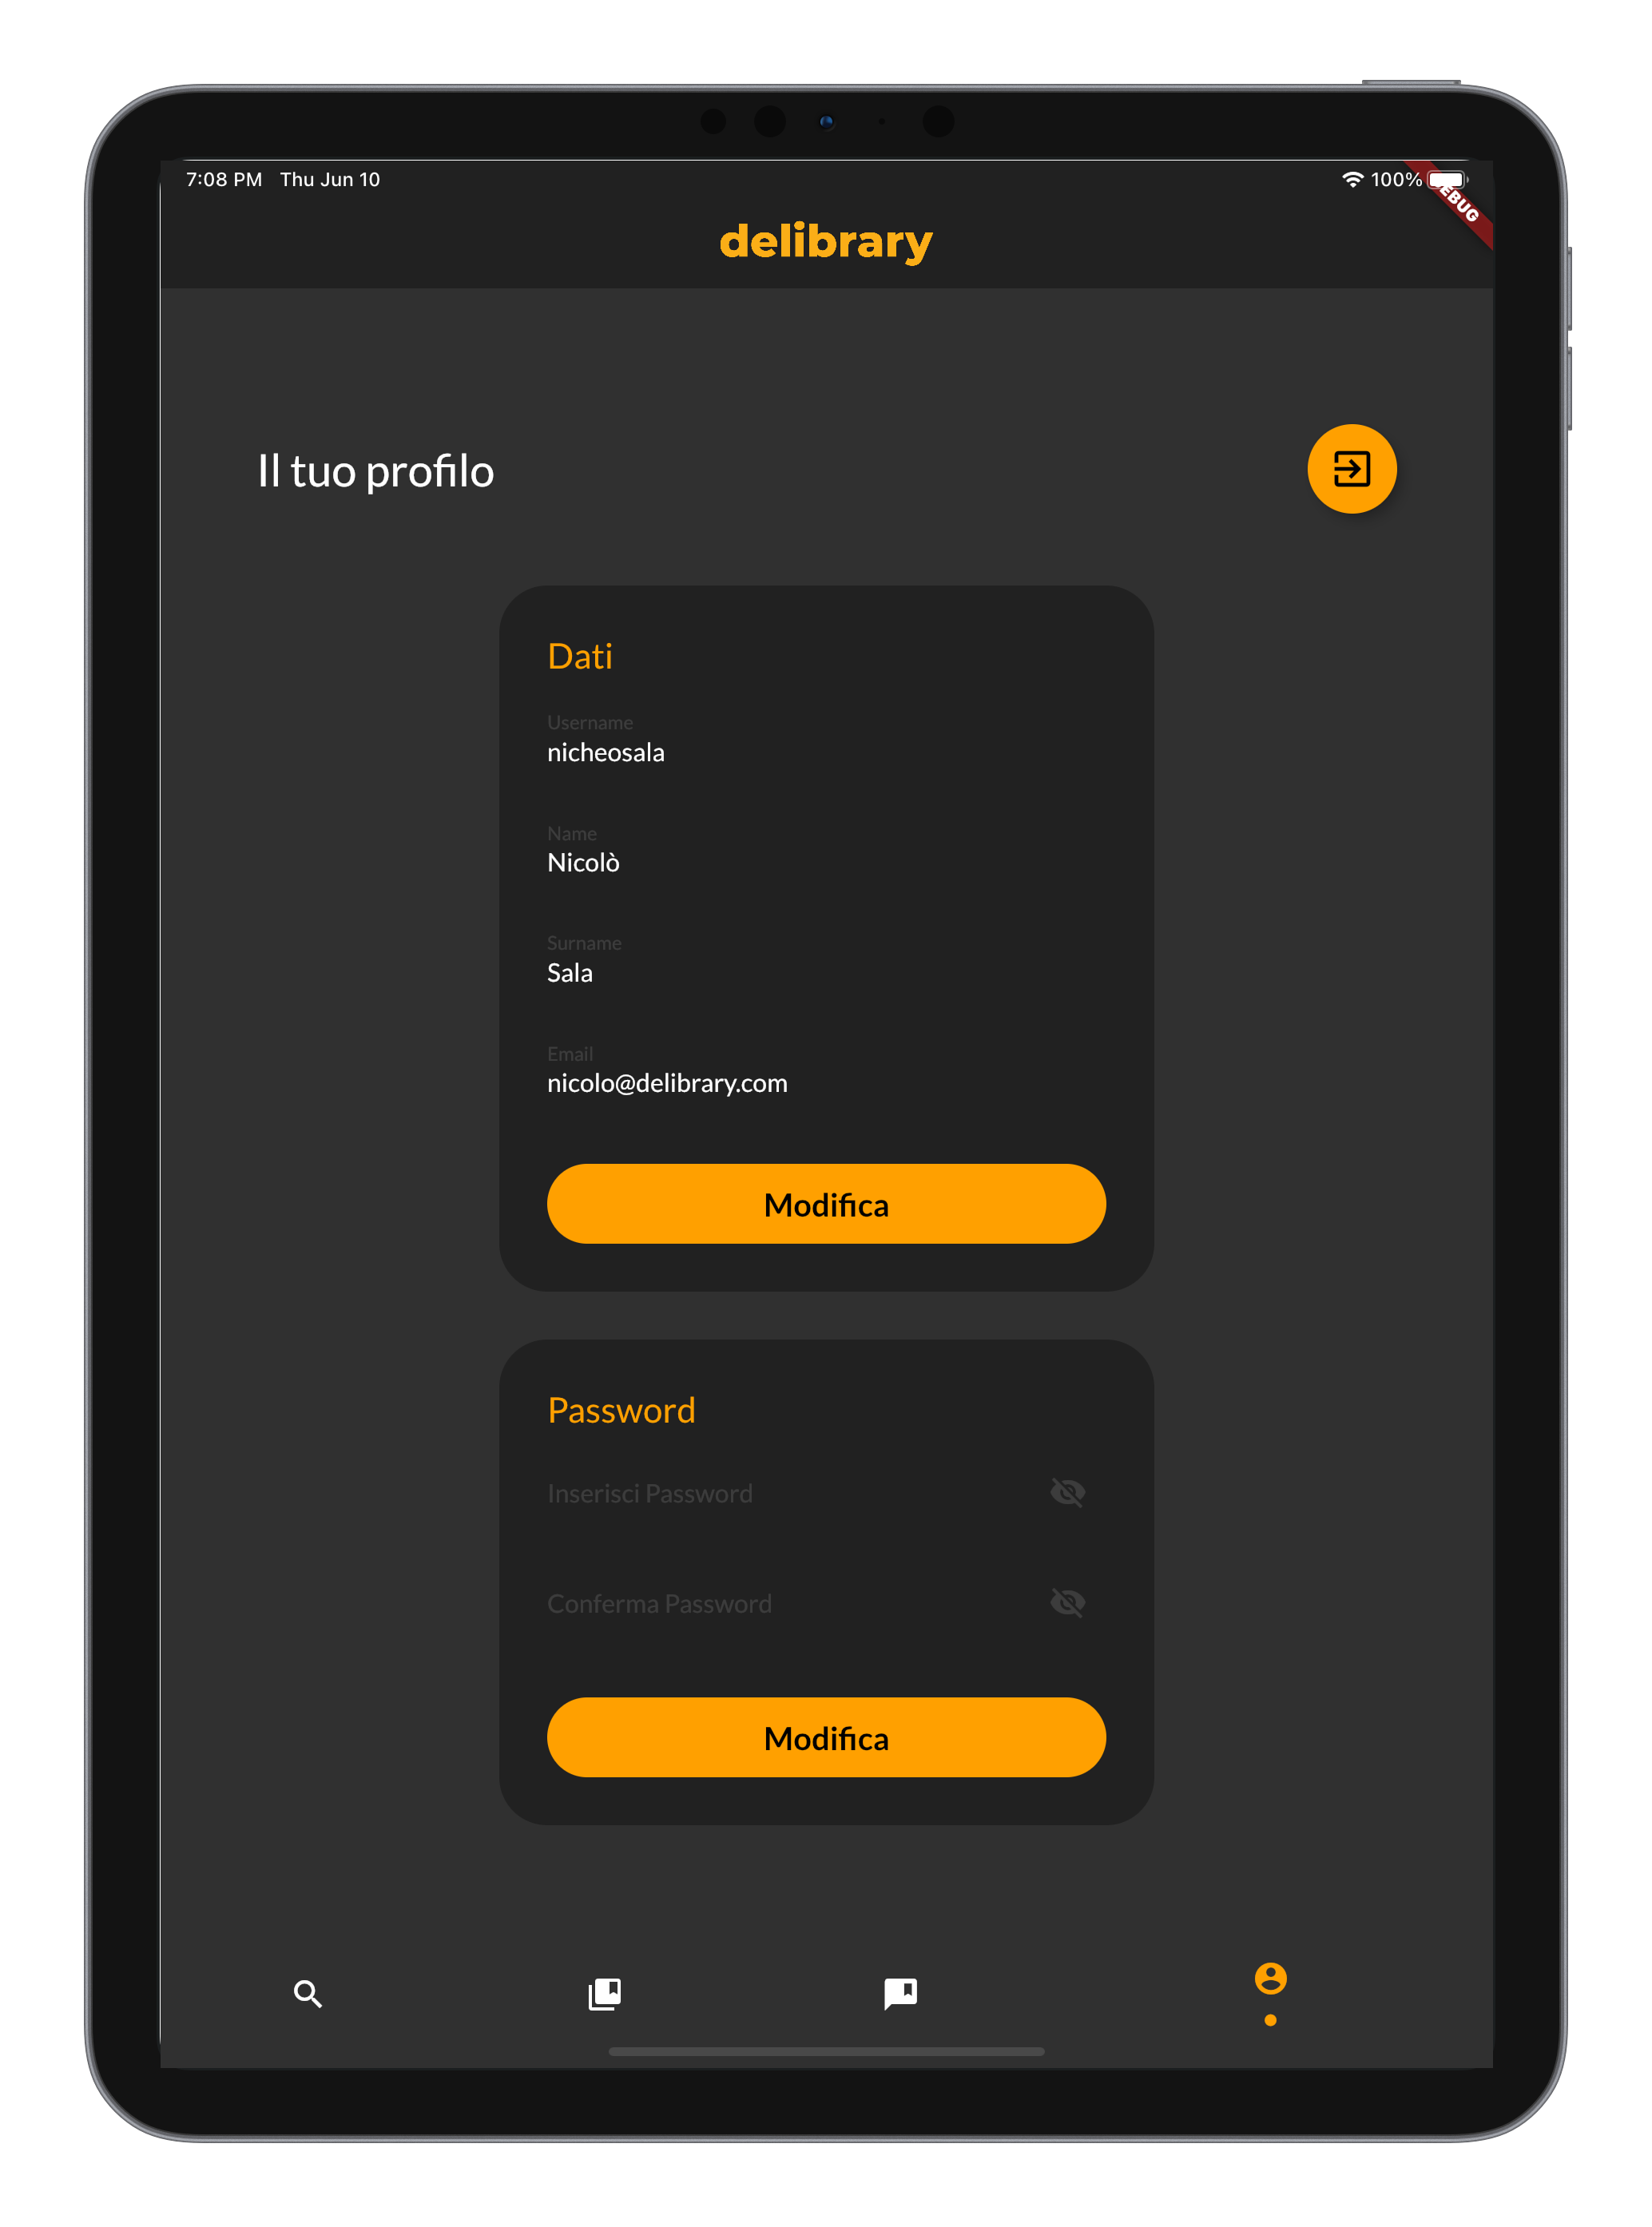
\includegraphics[width=0.54\textwidth]{screens/mock/tablet-portrait/profile.png}
      }
      \caption{Profile page}
\end{figure}



\chapter{Implementation, Integration and Test}

\section{Integration History}
We started the implementation of Delibrary defining the APIs of the web server through Swagger.
This choice allowed us to generate a Node.js server stub, exploiting Swagger Codegen.

Then, we modified the naïve web server so to connect it to PostgreSQL.
After that, it was possible to test the correctness of the server logic.
Running the web server locally and using the API web interface of Swagger for convenience, we were able to make requests to the web server.

At this point, the web server was able to manage the registration of a new User and the addition and removal of Properties and Wishes.
When we had the impression to have a good backend structure, we published it to Heroku.
Then we started working on the frontend, writing the skeleton of Delibrary mobile application, exploiting Flutter.

The app was implemented so to distinguish its functionalities in tabs. This allowed us to start working in parallel on different tasks.
In particular, one of us focused on the design of the app and on User authentication, while the other worked on the communication between client and server.

When Delibrary was able to fully manage User, Property and Wish, we started working on Exchange.
We knew it was the most challenging and fundamental feature of Delibrary.
Being it based on the previously implemented logic, we decided to takle it after everything else.

A step-by-step implementation together with a step-by-step testing of the functinalities brought us to the actual version of Delibrary.

\section{Backend Tests}
The backend tests were done exploiting \href{https://mochajs.org}{Mocha}, an open-source JavaScript test framework running on Node.js, that allows to make test requests to the APIs.
The assertions are handled exploiting \href{https://www.chaijs.com/}{Chai} assertion library.

The tests were conducted following the documentation of the API: first the APIs regarding the object User were tested, then the ones about Wish and Property, and the ones about the Exchange object in the end.
A database separated from the main one is used for testing purposes.

For each API, there is a test of the `optimal case', where all the parameters are legal and respect the logic of Delibrary.
Then, there are some tests that delve into particular logical cases, mostly about the management of the status of an Exchange.
All the tests are passed and they've been a fundamental mean in order to discover bugs quickly.

\section{Frontend Tests}
Tests on the frontend were done following \textit{Flutter} guidelines and were automated using \href{https://api.flutter.dev/flutter/flutter_test/flutter_test-library.html}{Flutter Test} library.

First, we decided to perform unit tests on the whole model of our application.
The goal of unit tests is to verify the correctness of a unit of logic (single method or functionality) under different conditions.
In general, we tested our modules both to check that correct input results in the expected behavior and that incorrect input is handled without modifying the state of the model.

After this, we carried out widget tests for those components containing important logic.
In widget testing, the testing library wraps the widget that is under analysis in order to provide a \texttt{BuildContext} to it.
Then, the test environment performs a sequence of interactions (taps, scrolls, ...) and scans the screen in order to verify that the widget's UI appears and works as expected.

Also in this case, all tests are passed and have been crucial to catch bugs and to keep the application working at each phase of the developement process.



\chapter{Possible Extensions and Updates}
Even if our application is already able to meet all the requirements which were originally intended, we are aware that there are multiple functionalities that could be implemented and that would improve it.

In this chapter we list some aspects in which the system could be improved but that we were not able to tackle for a matter of timing.
These functionalities are left as a starting point for possible future changes in case the app is published.

\begin{itemize}
      \item \textbf{Secure login}: without plaintext passwords and using more advanced technologies to manage the session.
      \item \textbf{``Internal'' search by title, author or ISBN}: in this version, we only support location-based queries on our database of user properties.
      \item \textbf{Possibility to visit other users' profiles}: in order to push towards a more ``social'' imprint of the application.
      \item \textbf{Book filtering system}: to allow users to limit their search using particular parameters like the author or the genre.
\end{itemize}

\end{document}